\chapter{Numerical solution of Fredholm integrals using regularization}
In physics, many experimental data can be described theoretical by a Fredholm integral. To extract a physical interesting quantity the integral equation often has to be solved numerically. In many cases, this problem becomes ill-posed and an additional regularization technique has to be included in the analysis to obtain a stable solution. A general overview about regularization techniques can be found e.g. in \cite{Hansen1998,Hansen2000b,Gazzola2018,Scherzer2011,Kern2016}.

\nocite{Benvenuto2016,Gao2016,Hansen2016,Pedersen2014,Sen2014,Blanchet2013,Mroczka2013,Paul2013,
Mroczka2013,Liu2012,Zhenhai2012,Bauer2011,Debski2010,Hansen2008,Santos2007,Wang2007,Stribeck2006,Vestergaard2006,Tatchev2004,
Hansen2003,Castellanos2002,Pike2002,Bergmann2000,Hansen2000,Hansen2000a,Elliott1999,Weyerich1999,Mittelbach1998,Mulato1998,
Brunner-Popela1997,Durchschlag1997,Mulato1997,Tsao1997,Gilmore1996,Hansen1996,Kline1996,Krauthauser1996,Muller1996,Mulato1996,
Serimaa1996,Jakes1995,Jemian1994,Ross1994,Steenstrup1994,Svergun1994,Glatter1993,Svergun1993,Morrison1992,Svergun1992,
Glatter1991,Goldin1991,Hansen1991,Semenyuk1991,Svergun1991,Jakes1991,Jakes1990,Bricogne1988,Glatter1988,Magnani1988,Potton1988,Potton1988a,
Svergun1988,Jakes1988,Thomas1987,Xu1987,Luzzati1986,Jakes1986,Livesey1985,Walter1985,Kubota1985,Bricogne1984,Glatter1984,Provencher1984,
Skilling1984,Britten1982,Kratky1982,Provencher1982,Provencher1982a,Taupin1982,Glatter1981,Glatter1980,Glatter1980b,Moore1980,Glatter1979,
Provencher1978,Glatter1977,Vonk1976,Pusey1974,Debye1915,Larsen2018,Bressler2015}.

\section{Problem description}
Also scattering techniques often measure  a quantity which can be written in form of a Fredholm integral.
The Fredholm equation of the first kind is defined as

\begin{align}
\label{eq:Fredholm}
g(t)=\int _{a}^{b}K(t,s)f(s)\,\mathrm {d} s
\end{align}
and the problem is, given the continuous kernel function $K(t,s)$ and the function $g(t)$, which is often an experimental measurable quantity with an error bar, to find the function $f(s)$. Sometimes the values of the Kernel scale somehow with a power law $s^\alpha$. In such a case a more stable solution can be obtained by rewriting the problem as
\begin{align}
\label{eq:KernelScaling}
g(t)=\int _{a}^{b}s^{-\alpha} K(t,s) \, s^{\alpha}f(s)\,\mathrm {d} s
\end{align}
where now the continuous kernel function is defined as $s^{-\alpha}K(t,s)$ and the function to be determined $s^{\alpha} f(s)$.

One simple example is the smearing of the signal by a known resolution function. These folding integrals can in principle be solved in Fourier space. However, also the signal without any smearing are often described by a known or assumed function with one parameter having a distribution. The resulting signal is than an integral of the product of the known function and the probability distribution which one likes to determine. In both cases these integrals belongs to Fredholm integrals of first kind.

In small angle scattering the measured intensity $I_m$ is given as a function of the scattering vector $q=4\pi\sin(\theta)/\lambda$, with $\theta$ being the scattering vector and $\lambda$ the wavelength of the probing radiation. The smearing by limited resolution resolution for a pinhole came can be written as
\begin{equation} \label{eq:res}
I_m(\langle Q\rangle) = \int_0^\infty R_{av}\left(Q,\langle
Q\rangle,\sigma\right) I(Q) \, \mathrm{d}Q
\end{equation}
where $R_{av}\left(Q,\langle Q\rangle,\sigma\right)$ describes the known resolution function and $\sigma$ the resolution parameter, which is known for each measured $\langle Q\rangle$-value \cite{Pedersen1990}. A desmearing of the data could help to accelerate the analysis as the model does not need to be folded anymore with the resolution function.

Typical tasks in the analysis of desmeared data are to determine size distribution $N(s)$, pair distribution functions $p(r)$ or scattering length density profiles $\rho$.

\subsection{Size distribution $N(R)$}
\label{sec:N(R)}

The size distribution can be determined, if the particle shape is known. For many particle shapes the scattering intensity or form factor can be calculated via an analytical expression. The scattering intensity are than describes by integrating the squared form factor $F^2(Q,s)$ over a distribution function $N(s)$, where $s$ describes the size of the scattering objects \cite{Pedersen1997}. The intensity is than given by
\begin{equation} \label{eq:SD}
I(Q) = \int_0^\infty N(s) \abs{F(Q,s)}^2 \, \mathrm{d}s
\end{equation}
To solve equation \ref{eq:SD} one often parameterize the size distribution by assuming an analytical distribution function like LogNormal, Gaussian, Weibull or Schulz-Zimm distribution, with a few input parameter and is fitting these parameters by performing the numerical integration and applying a Levenberg-Marquardt strategy to solve a non-linear least square problem \cite{Bressler2015}. This however assume a priori knowledge about the distribution function. More desirable would be a discretization of the size distribution $N_i$ at the positions $s_i$ and determine all $N_i$ without any further assumption. This however is normally an ill posed problem and requires some additional regularization to determine a unique solution for the vector $N_i$. By discretization of the problem one also can easily include the resolution function. As the resolution function only depends on the scattering vector $Q$ and not on the particle size $s$ the order of integrations over the size distribution and the resolution function can be changed as all functions are continuous and integrable. Combining eq.\ \ref{eq:res} and \ref{eq:SD} yields
\begin{align}
I_m(\langle Q\rangle) &= \int_0^\infty R_{av}\left(Q,\langle
Q\rangle,\sigma\right)  \int_0^\infty N(s) \abs{F(Q,s)}^2 \, \mathrm{d}s \, \mathrm{d}Q \\
&= \int_0^\infty N(s)  \int_0^\infty R_{av}\left(Q,\langle
Q\rangle,\sigma\right) \abs{F(Q,s)}^2 \, \mathrm{d}Q \, \mathrm{d}s \label{eq:IQ}
\end{align}
As already mentioned in eq.\ \ref{eq:KernelScaling} also here the squared form factor is scaling with the squared sample volume, which is in the case of spheres proportional to $R^6$. Therefore the distribution function to be determined often is choosen to be the intensity distribution $N(R)R^\alpha$ with $\alpha=6$ so that eq.\ \ref{eq:IQ} is slightly modified to
\begin{align}
I_m(\langle Q\rangle) &=  \int_0^\infty N(s)s^\alpha  \int_0^\infty R_{av}\left(Q,\langle
Q\rangle,\sigma\right) s^{-\alpha}\abs{F(Q,s)}^2 \, \mathrm{d}Q \, \mathrm{d}s
\end{align}
which can be written as a linear matrix equation by discretization
\begin{align}
\label{eq:discreteFredholm}
b_i &= \sum_{j=0}^{N-1} A_{i,j} x_j \\
\label{eq:discreteFredholmVector}
\mathbf{b} &= \hat{\mathbf{A}}\mathbf{x}
\end{align}
with $\hat{\mathbf{A}}$ being a $M\times N$ matrix, $\mathbf{b}$ a vector of length $M$ and $\mathbf{x}$ a solution vector of length $N$ where their elements are given by
\begin{align}
x_j &= N(s_j) s_j^{\alpha}\\
b_i &= I(\langle Q\rangle_i) \\
A_{i,j} &= \Delta s_j \int_0^\infty R_{av}\left(Q,\langle Q\rangle_i,\sigma_i\right) s_j^{-\alpha} \abs{F(Q,s_j)}^2 \, \mathrm{d}Q  \label{eq:AijFF}
\end{align}
$R_{av}\left(Q,\langle Q\rangle_i,\sigma_i\right)$ and $s_j^{-\alpha}\abs{F(Q,s_j)}^2$ are known functions, so that the integral only has to be calculated once for each pair of $(\langle Q\rangle_i,s_j)$.


\subsection{Pair distance distribution function $p(r)$}
\label{sec:p(r)}

The above formalism is often applied if a priori knowledge about the shape of the scattering objects is available but not about their size distribution. If the shape of the scattering objects is also not known one often like to convert the intensity data from $Q$-space into $r$-space by calculating the pair distance distribution function. The scattering intensity is the square of the Fourier transformation of the scattering length density $\rho(\mathbf{r})$
\begin{align}
I(\mathbf{Q}) &= \abs{\int_0^\infty \rho(\mathbf{r}) \exp(-\imath \mathbf{Q r}) \, \mathrm{d}\mathbf{r}}^2  \\
              &= \int_0^\infty \mathrm{d}\mathbf{r} \,  \exp(-\imath \mathbf{Q r}) \int_0^\infty \mathrm{d}\mathbf{r_1}\, \rho(\mathbf{r_1}) \overline{\rho}(\mathbf{r_1}-\mathbf{r}) \\
              & \int_0^\infty \mathrm{d}\mathbf{r} \,\exp(-\imath \mathbf{Q r}) \gamma(\mathbf{r})
\end{align}
where $\gamma(\mathbf{r})$ is the autocorrelation function of the scattering length density. For isotropic media without texture the autocorrelation only depends on the modulus of $r$ so that one obtains
\begin{align}
I(Q) &= \int_0^\infty 4\pi r^2 \gamma(r) \frac{\sin(Qr)}{Qr} \mathrm{d}r\\
     &= 4\pi \int_0^\infty p(r) \frac{\sin(Qr)}{Qr} \mathrm{d}r \label{eq:Isp}
\end{align}
with $p(r)= r^2 \gamma(r)$ being the pair distance distribution function. This function is calculated first by many people analysing SAS data and afterwards interpreted further. For the scattering intensity of objects with cylindrical symmetry and planar symmetry but random orientation one finds corresponding expressions:
\begin{align}
I_\mathrm{cyl}(Q) &= 2\pi^2 L \int_0^\infty p(r) \frac{J_0(Qr)}{Q} \, \mathrm{d}r \label{eq:Icyl} \\
I_\mathrm{plan}(Q) &= 4\pi A \int_0^\infty p(r) \frac{\cos(Qr)}{Q^2} \, \mathrm{d}r \label{eq:Ipl}
\end{align}
where $J_0$ is the Bessel function of zero order, $L$ the length of the cylindrical object and for planar structures $A$ is the are of the object. The pair distance distribution function $p(r)$ is related to the correlation function $\gamma(r)$through
\begin{align}
p(r) &= r^{\mathrm{dim}-1} \gamma(r)
\end{align}
Here $\mathrm{dim}$ denotes the symmetry of the scatterer (1: planar, 2: cylindrical, 3: spherical) and
\begin{align}
\gamma(r) = \int_{-\infty}^{\infty} \rho(x)\rho(x-r)\,\mathrm{d}x
\end{align}
where $\rho(r)$ is the scattering length density distribution. For one-dimensional symmetry $r$ is the normal distance from the plane, for two-dimensional symmetry the normal distance to the cylinder axis and for three-dimensional symmetry the distance from the center of the sphere.
The integrals (\ref{eq:Isp}), (\ref{eq:Icyl}) and (\ref{eq:Ipl}) can be discretized on the grid $r_i$ so that one obtains the matrix equation
\begin{align}
b_i &= A_{i,j} x_j \\
A_{i,j}^\mathrm{sp} &= \Delta r_j \frac{\sin(Q_i r_j)}{Q_i r_j}\\
x_j &= p(r_j) r_j^{\alpha}\\
b_i &= I(\langle Q\rangle_i) \\
\end{align}
Also here the resolution function can be easily include likewise as in \ref{eq:AijFF}. In this case normally no resclaing is done and $\alpha=0$ is chosen.

\subsection{Size distribution $N_h(R_h)$ from dynamic light scattering}
\label{sec:DLS}
In dynamic light scattering (DLS) the scattering intensity is measured as a function of time. With a coherent lase beam one obtains a speckle pattern from the sample which is fluctuating due to Brownian motions. The intensity autocorrelation function $g_{(2)}(q,\tau)=\int  I(q,t) I(q,t+\tau)\,\mathrm{d}t/\left(\int  I^2(q,t)\,\mathrm{d}t\right)$. The Siegert equation relates the second-order autocorrelation function $g_{(2)}(q,\tau)$ (intensity autocorrelation) with the first-order autocorrelation function $g_{(1)}(q,\tau)$ (amplitude autocorrelation) as follows:
\begin{align}
    \label{eq:siegert}
    g_{(2)}(q,\tau)= A+\beta\left[g_{(1)}(q,\tau)\right]^2
\end{align}
In an ideal experiment $A=1$ and $\beta=1$. For monodisperse spherical particles the first order autocorrelation function decays as a single exponential decay
\begin{align}
    g_{(1)}(q,\tau) &= \exp\left(-\Gamma\tau\right)
\end{align}
where $\Gamma$ is the decay rate, which is related to the translational diffusion coefficient $D_t$ and may be derived at a single angle or at a range of angles depending on the wave vector $q$. They are related by
\begin{align}\label{eq:GammaDq2}
\Gamma &=q^2D_t
\end{align}
with
\begin{align}
\label{eq:q}
 q &= \frac{4\pi n_0}{\lambda}\sin\left(\frac{\theta}{2}\right)
\end{align}
where $\lambda$ is the incident laser wavelength, $n_0$ is the refractive index of the sample and $\theta$ is angle at which the detector is located with respect to the sample cell. The translational diffusion coefficient depends via the Stokes-Einstein relation on the hydrodynamic radius $R_h$ of the particle and the viscosity $\eta$ of the carrier liquid
\begin{align}
\label{eq:D_t}
D_t &= \frac{k_BT}{6\pi\eta R_h}
\end{align}

In most cases, samples are polydisperse. Thus, the amplitude autocorrelation function is a sum of the exponential decays corresponding to each of the species in the population.
\begin{align}
    g_{(1)}(q,\tau) &= \sum_{i=1}^n G_i(\Gamma_i)\exp(-\Gamma_i\tau) = \int G(\Gamma)\exp(-\Gamma\tau)\,d\Gamma.
\end{align}
 Since $G(\Gamma)$ is proportional to the relative scattering from each species, it contains information on the distribution of sizes. Unfortunately the amplitude autocorrelation function is not directly experimentally accessible. Experimentally available is the intensity autocorrelation function (see eq.\ \ref{eq:siegert}). Many hardwares for autocorrelation automatically determine the baseline and supply a reduced intensity autocorrelation
 \begin{align}
 g_{(2)}(\tau)-1 &=\abs{g_{(1)}(\tau)}^2 = \abs{\int_0^\infty G(\Gamma) \exp(-\Gamma\tau)\,\mathrm{d}\Gamma}^2
 \end{align}
 For the analysis one has to calculate first $g_{(1)}(\tau)$ from $g_2(\tau)-1$. Often one just takes the square root of the reduced intensity autocorrelation to obtain the amplitude autocorrelation. As the amplitude autocorrelation function is always positive this is justified. However, due to noise the reduced intensity autocorrelation can also become negative for large relaxation times $\tau$ as $g_2(\tau)-1=\abs{g_1(\tau)}^2 \rightarrow 0$ for $\tau\rightarrow\infty$. Simply neglecting negative reduced intensities autocorrelation values would produce systematic errors in the analysis. A more stable and reliable strategy, even though badly mathematically justified, is to set
\begin{align}
\label{eq:sqrt_g2m1}
 g_{(1)}(\tau) &= \mathrm{sign}(g_{(2)}(\tau)-1) \sqrt{\abs{g_{(2)}(\tau)-1}}
\end{align}
Another strategy is to make use of the faltungs theorem for Laplace transform.
\begin{align}\label{eq:Lg2}
 g_{(2)}(\tau)-1 &=\abs{g_{(1)}(\tau)}^2 = \int_0^\infty G(x) \exp(-x\tau)\,\mathrm{d}x \times \int_0^\infty G(y) \exp(-y\tau)\,\mathrm{d}y
 \end{align}
 Changing the variable $x+y=z$ one gets
\begin{align}
 \abs{g_{(1)}(\tau)}^2 &= \int_y^\infty G(y) G(z-y)\exp(-z\tau)\,\mathrm{d}y\mathrm{d}z \\
                   &= \int_0^\infty G_{(2)}(z) \exp(-z\tau)\,\mathrm{d}z = \mathcal{L}\left[G_{(2)}(\Gamma)\right]
 \end{align}
where $G_{(2)}(\Gamma)=\int_{-\infty}^\infty G(y) G(z-y) \mathrm{d}y$ and $\mathcal{L}\left[\right]$ denotes the Laplace transform. The faltung theorem for the Laplace transform leads to
\begin{align}
 \mathcal{L}\left[\int_{-\infty}^\infty G(y) G(z-y) \mathrm{d}y\right] &= \mathcal{L}\left[G(y)\right] \mathcal{L}\left[G(y)\right]
\end{align}
Pike \cite{Pike2002}  suggests to calculate first $G_2(\Gamma)$ but than taking the square root of the Laplace transformation and afterwards the inverse of that square root
\begin{align}
G(\Gamma) &=
\mathcal{L}^{-1}\left[\sqrt{\mathcal{L}\left[G_{(2)}(\Gamma)\right]}\right]
\end{align}
The determination of $G_{(2)}(\Gamma)$ is also done by an inverse Laplace transform. However, this first transform can be done by regularization techniques. The other two are done directly. Pike \cite{Pike2002} mentions that this looks as one has "gone around in a circle since, by cancelling out the two transforms under the square root, this is nothing but the original method" but also that "One can hardly dispute the experimental results
that show a significant improvement in accuracy".


 Goldin \cite{Goldin1991} is suggesting a mixture of both methods. He has shown that even when the value under the radical in eq.\ \ref{eq:sqrt_g2m1} is non-negative, calculating $g_1(\tau)$ from $\sqrt{g_2(\tau)-1}$ increases the random error (relative to $g_2(\tau)$ and introduces a systematic error. He proposes to compute the distribution of interest in two stages. In the first stage, the self-convolution of the distribution of interest $G_{(2)}(\Gamma)$ is computed from the function $g_2(\tau)-1$ like in \cite{Pike2002}. The smoothed estimation of $g_2(\tau)$ is then computed and used to compute the first order correlation function $g_1(\tau)$. This is than used to calculate $G(\Gamma)$.

After determining the relaxation probability $G(\Gamma)$ function the size distribution function $N_h(R_h)$ has to be determined. The relaxation time $\Gamma$ and the hydrodynamic radius are related via eq.\ \ref{eq:GammaDq2}, \ref{eq:q}, and \ref{eq:D_t}
\begin{align}
\Gamma = \Gamma(R_h)&= q^2 \frac{k_BT}{6\pi\eta R_h}
\end{align}
Furthermore the the scattering intensity of the particle $I(q,R_h)$ also contributes as a weighting factor, i.e. how much a certain size contributes to the relaxation distribution function of the corresponding relaxation time $G(\Gamma)$.
\begin{align}
\label{eq:GRh}
G(\Gamma) &= \frac{I(q,R_h) N_h(R_h) \Gamma(R_h)} {\int_0^\infty I(q,R_h) N_h(R_h) \, \mathrm{d}R_h}
\end{align}
so that the size distribution of the hydrodynamic radius is proportional to
\begin{align}
\label{eq:Nh}
N_h(R_h) &\propto  \frac{G\left(q^2 \frac{k_BT}{6\pi\eta R_h}\right)}{\int_0^\infty I(q,R_h) N_h(R_h) \, \mathrm{d}R_h}
\end{align}
The volume and intensity distribution $N_v(R_h)$ and $N_i{R_h}$ are than defined as
\begin{align}
N_v(R_h) &= R_h^3 N_h(R_h) \\
N_i(R_h) &= R_h^6 N_h(R_h)
\end{align}
Eq.\ \ref{eq:Nh} or eq.\ \ref{eq:GRh} show, that the size distribution or decay rate distribution also depend on the $q$ and size dependent scattering function $I(q,R_h)$. Analysing intensity correlation function at different angles simultaneously normally helps to get a more stable solution for the size distribution of particles.

\section{Expectation Maximization (EM)}
The EM algorithm has been first explained in \cite{Dempster1977}. The method is an iterative fixed point method for positive defined functions. (Other fixed point techniques are described for example in \cite{Hanke2000}.) In \cite{Vardi1993} it has been shown how the EM method can be applied to solve Fredholm integrals for the domain of nonnegative real valued functions. The method described there is equivalent to the Lucy\hyp{}Richardson method \cite{Richardson1972,Lucy1974}. For calculating size distribution from scattering data the method has been applied e.g.\ by \cite{Yang2013,Benvenuto2016,Benvenuto2017,Bakry2019}. For inverting scattering data to pair distance distribution functions the condition of nonnegativity of the involved functions does not hold anymore as both the kernel of the Fredholm integral as well as the pair distance distribution function can take negative values. In \cite{Chae2018} it has been shown, how the EM algorithm can be reformulated for non-density functions, i.e. to functions which also can take negative values.

Writing the Fredholm integral in eq.\ \ref{eq:Fredholm} or \ref{eq:KernelScaling} in discrete form according to \ref{eq:discreteFredholm}
\begin{align}
b_i &= \sum_{j=0}^{N-1} A_{i,j} x_j
\end{align}
the EM iteration scheme or Lucy\hyp{}Richardson inversion method reads as
\begin{align}\label{eq:LucyRichardsonInversionMethod}
  x_j^{(k+1)} &= x_j^{(k)} + \Delta x_j^{(k)} = \mathcal{O}_\mathrm{EM}\left[x_j^{(k)}\right]\\
  \Delta x_j^{(k)} &= x_j^{(k)}\left[\sum_{i=0}^{M-1}\frac{A_{ij}}{\left(\displaystyle \sum_{m=0}^{M-1}A_{mj}\right)}\frac{b_i}{\displaystyle \sum_{n=0}^{N-1}A_{in}x_n^{(k)}}-1\right]
\end{align}
where $\mathcal{O}_\mathrm{EM}$ is the fixed point operator. It has been shown, that the convergence is assured since the algorithm is guaranteed to increase the likelihood at each iteration. On the other side the algorithm is known to converge quite slow.


\begin{figure}[htb]
\centering
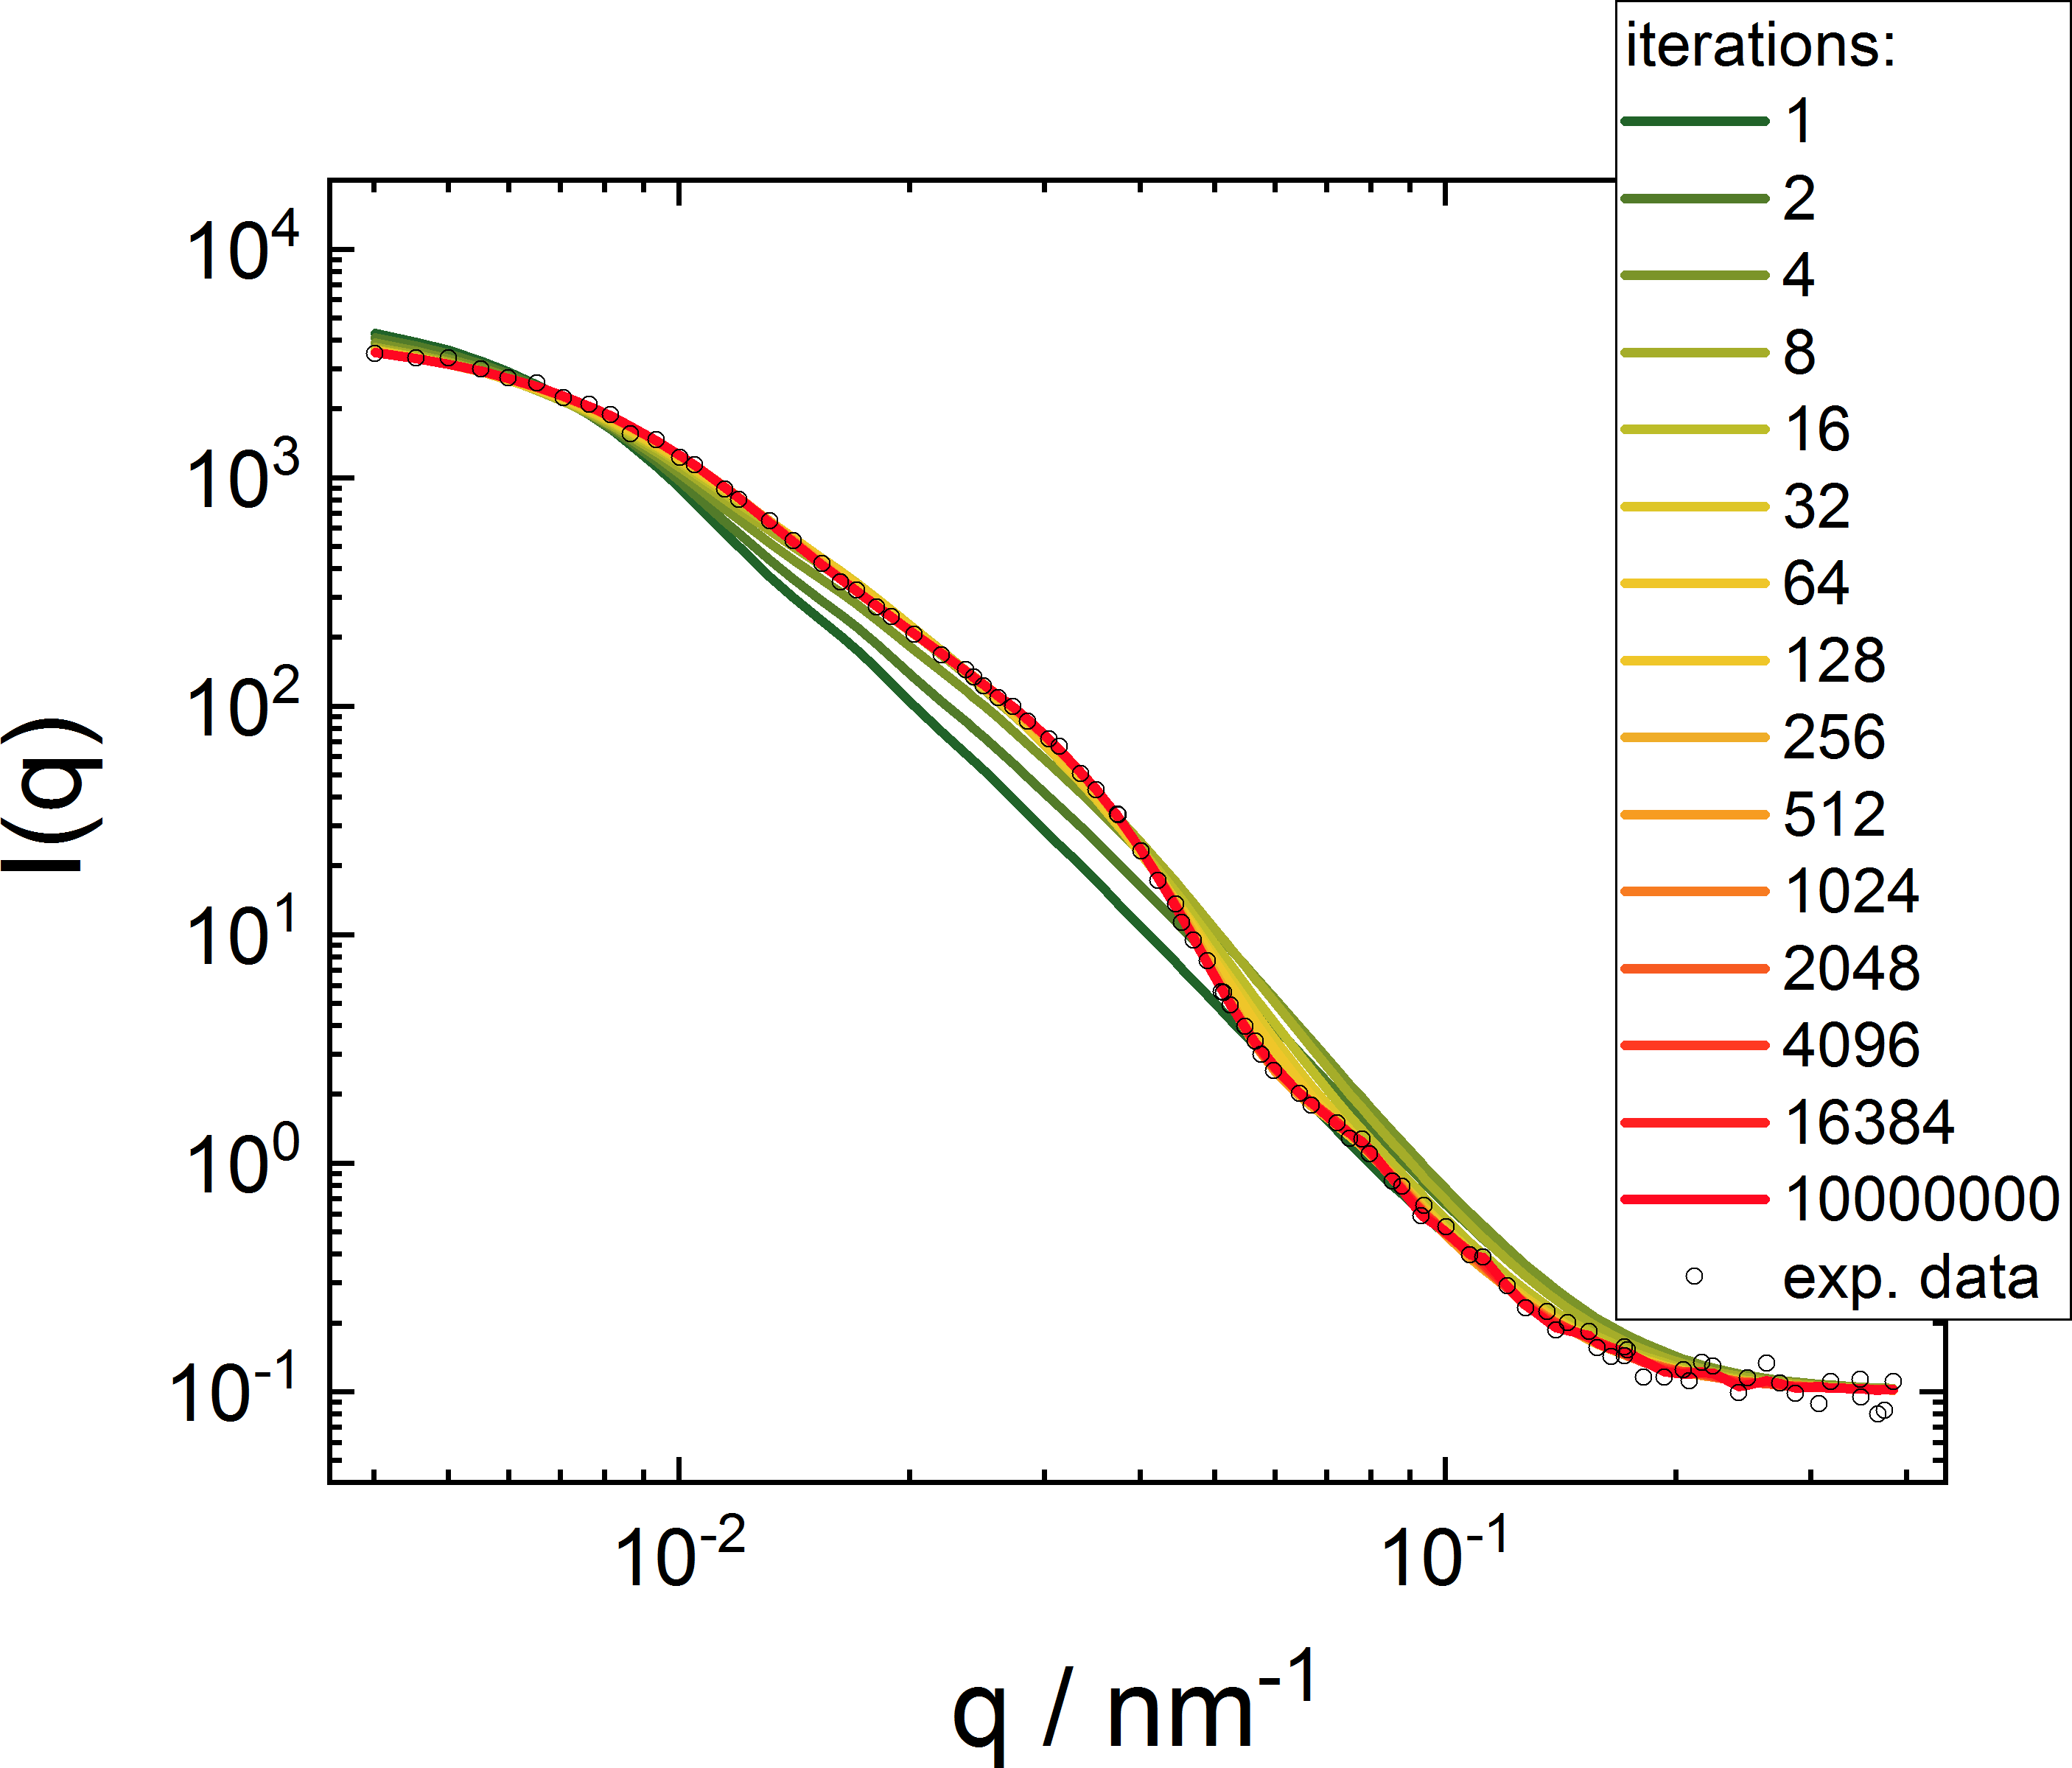
\includegraphics[width=0.46\textwidth]{../images/form_factor/EM/EMconstant_seed_smooth_0_0_IQ.png}
\hspace{0.06\textwidth}
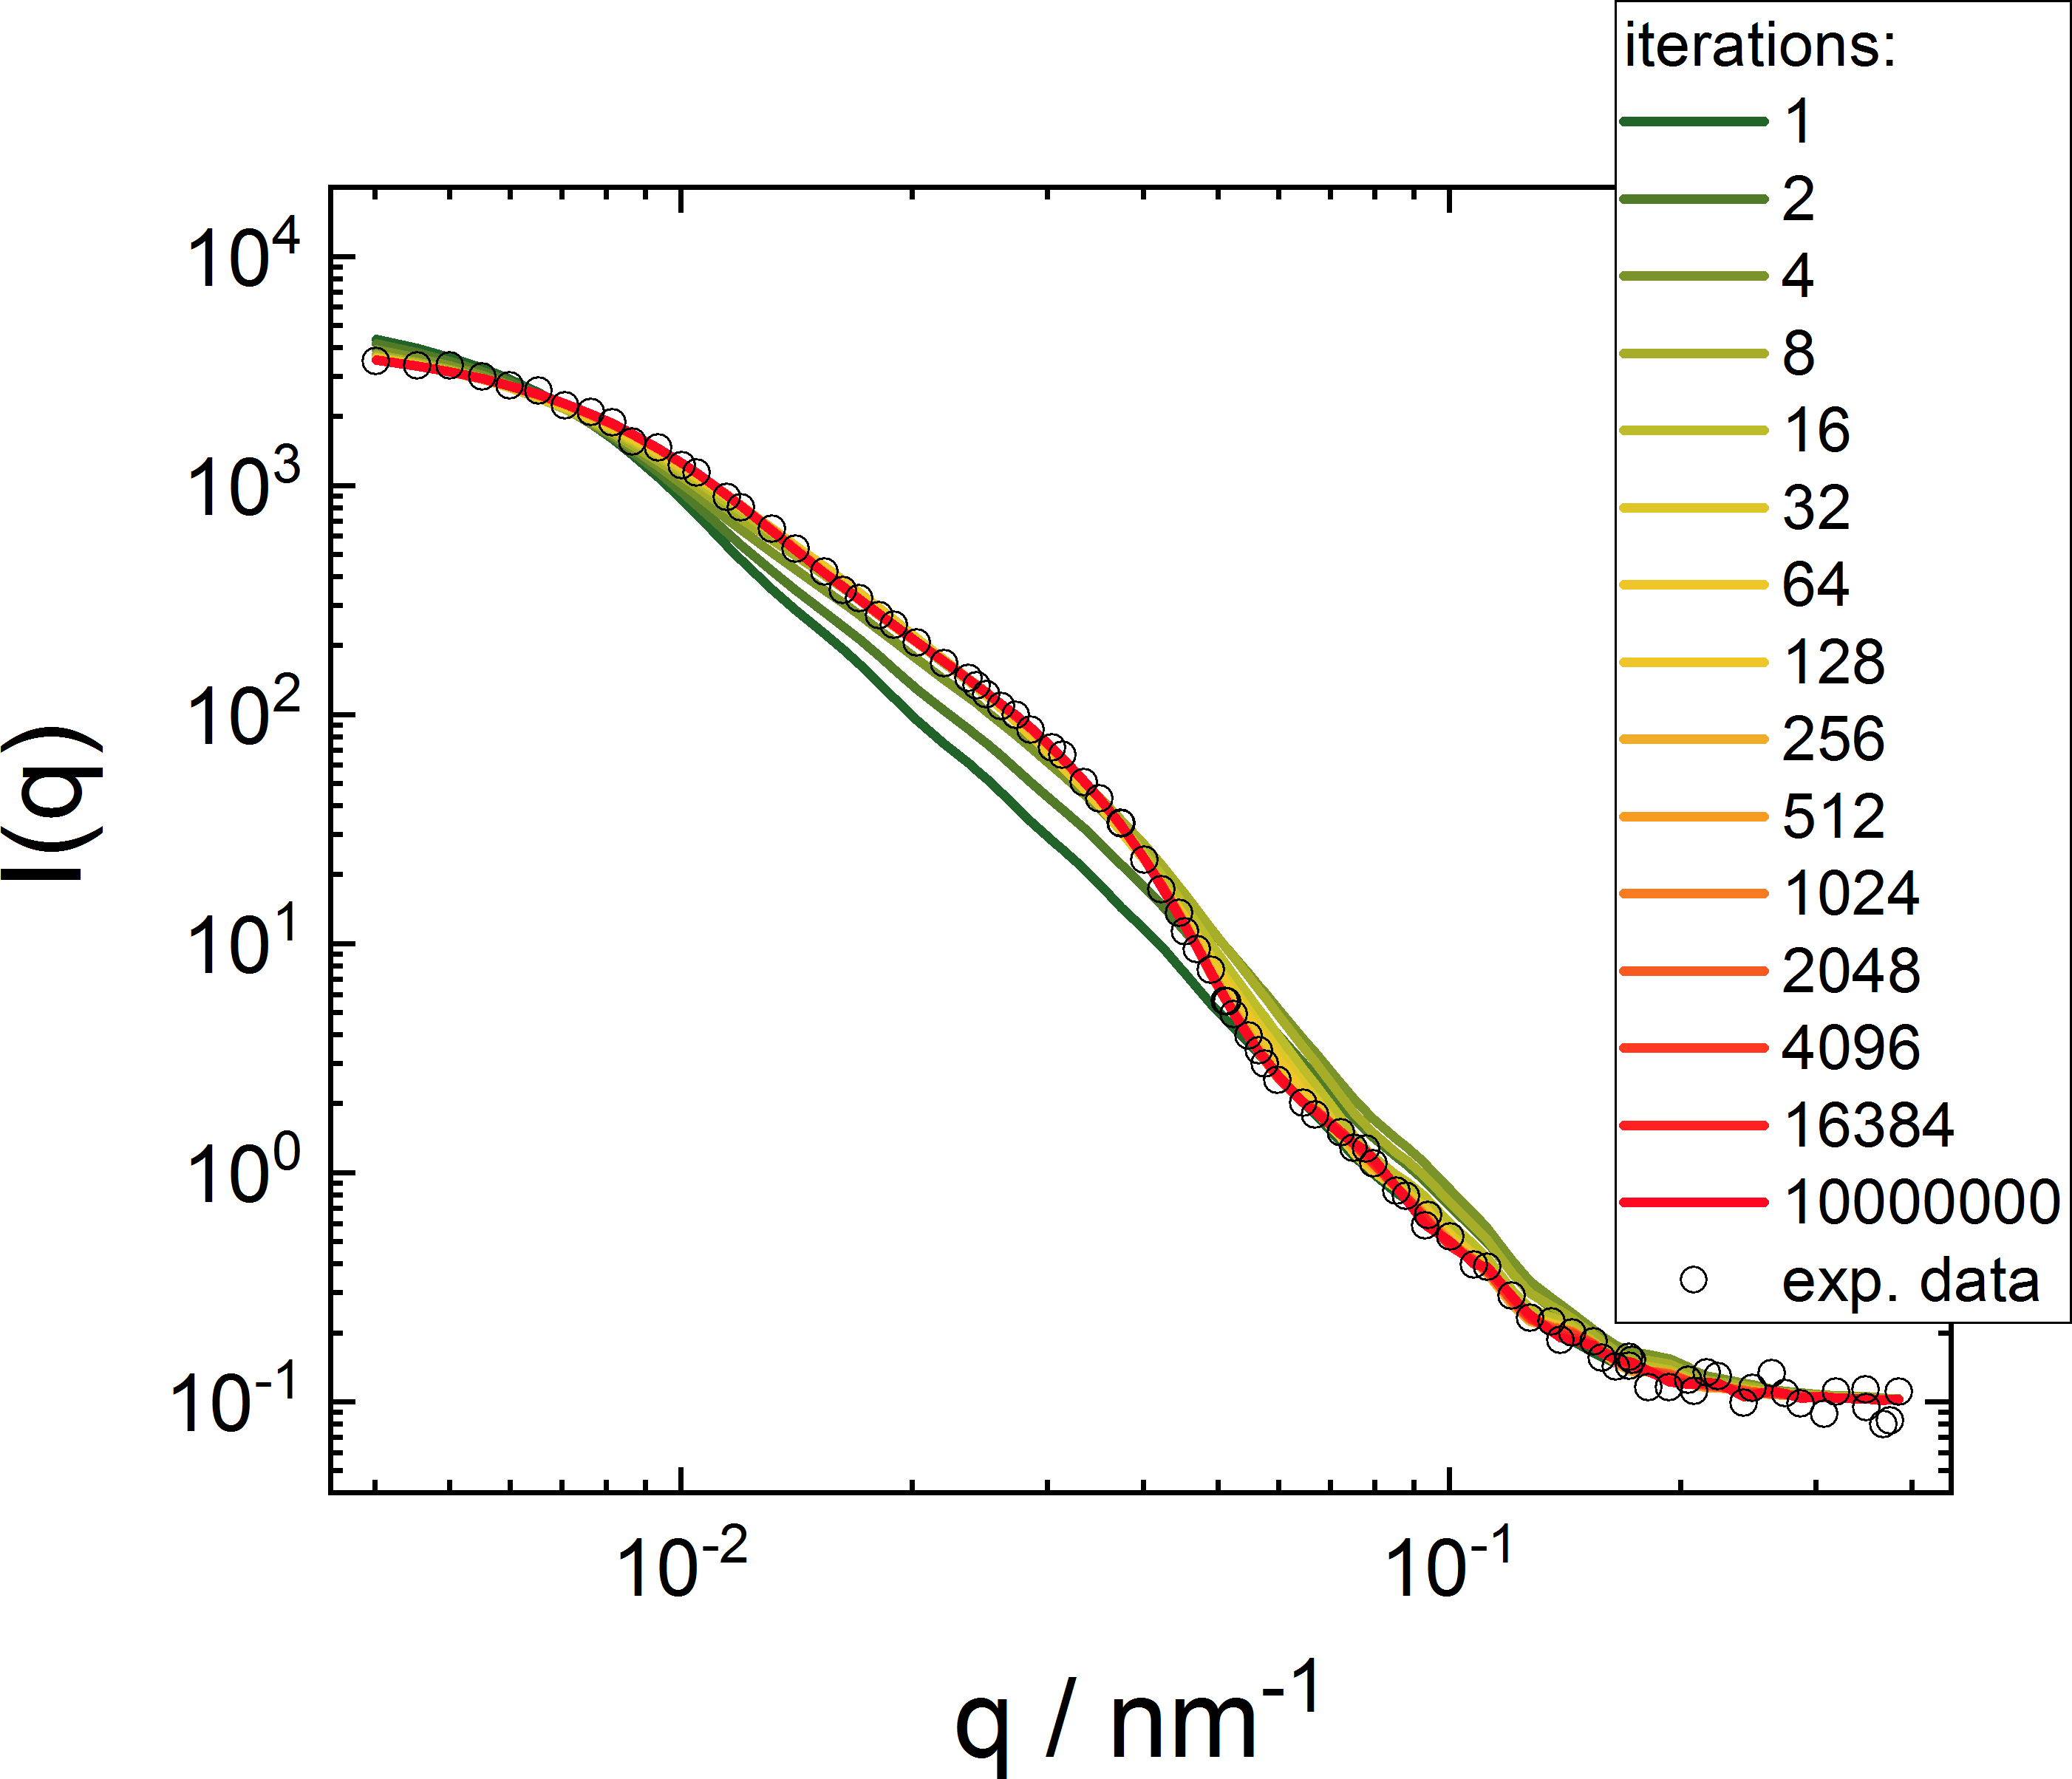
\includegraphics[width=0.46\textwidth]{../images/form_factor/EM/EMrandom_seed_smooth_0_0_IQ.png}
\caption{Scattering curve evolution for increasing number of iterations for a constant seed value (left) and random seed values (right).\label{fig:EMIQevolution}}
\end{figure}

\begin{figure}[htb]
\centering
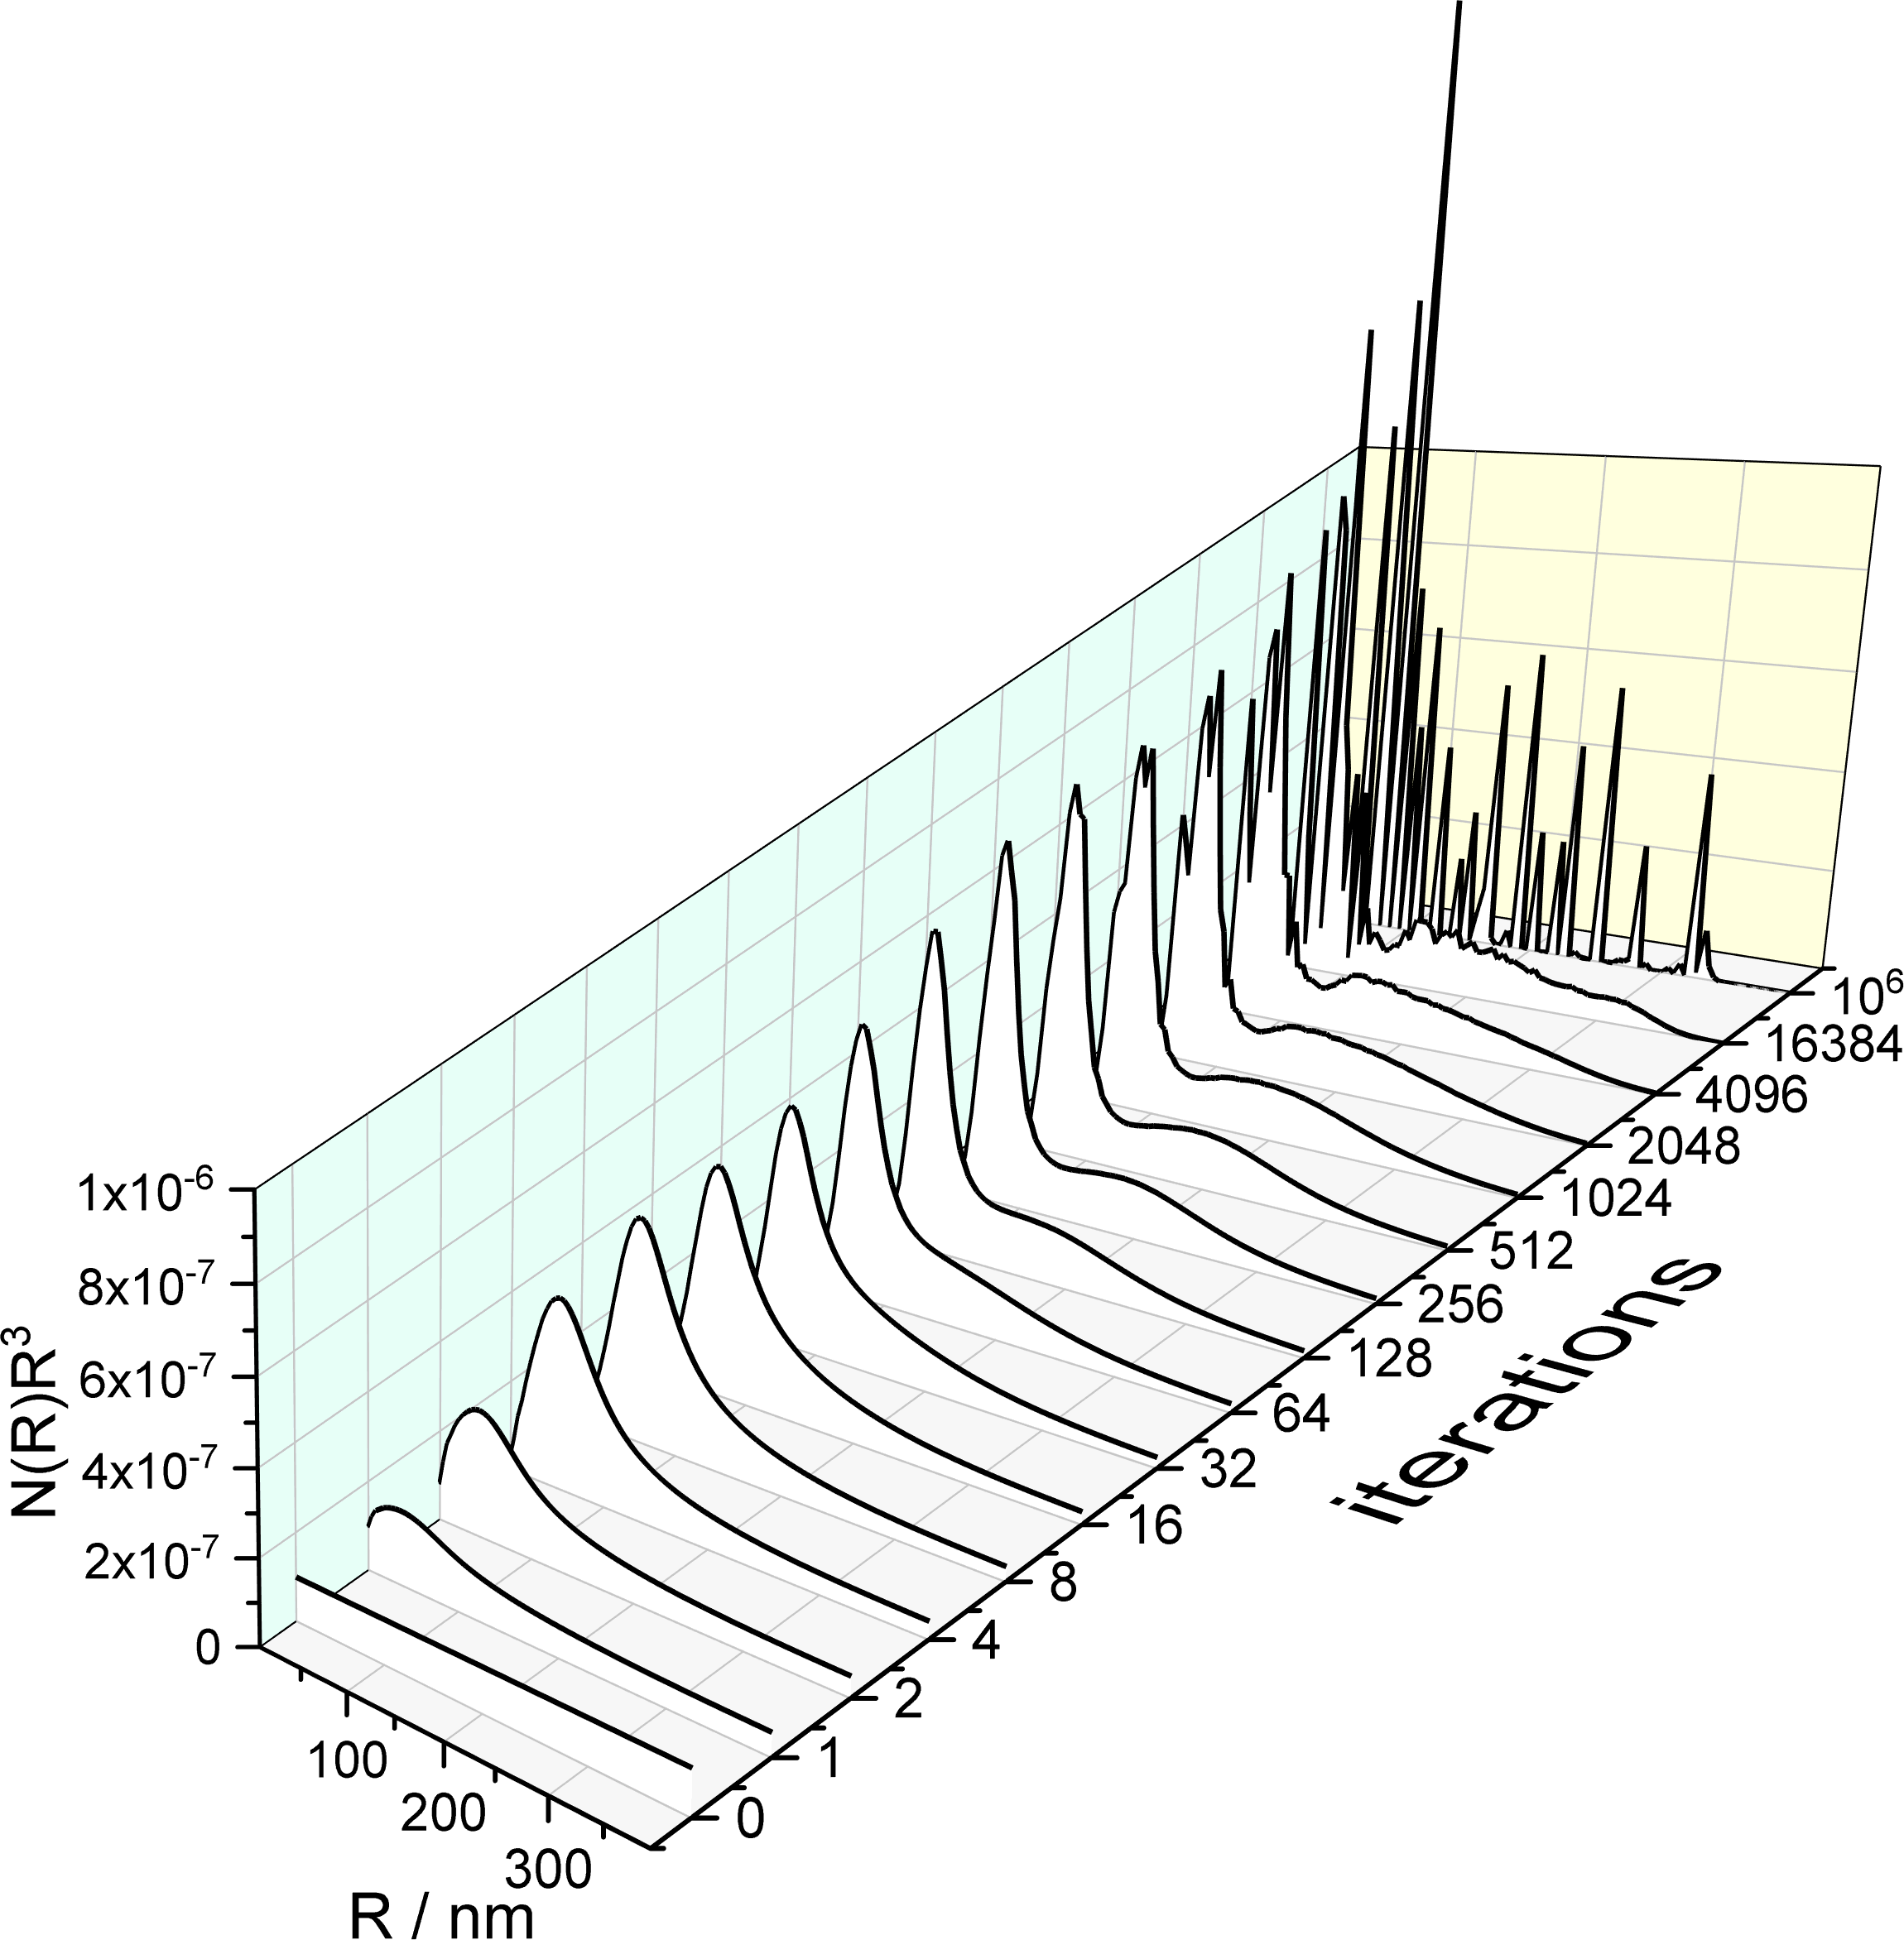
\includegraphics[width=0.46\textwidth]{../images/form_factor/EM/EMconstant_seed_smooth_0_0_NR.png}
\hspace{0.06\textwidth}
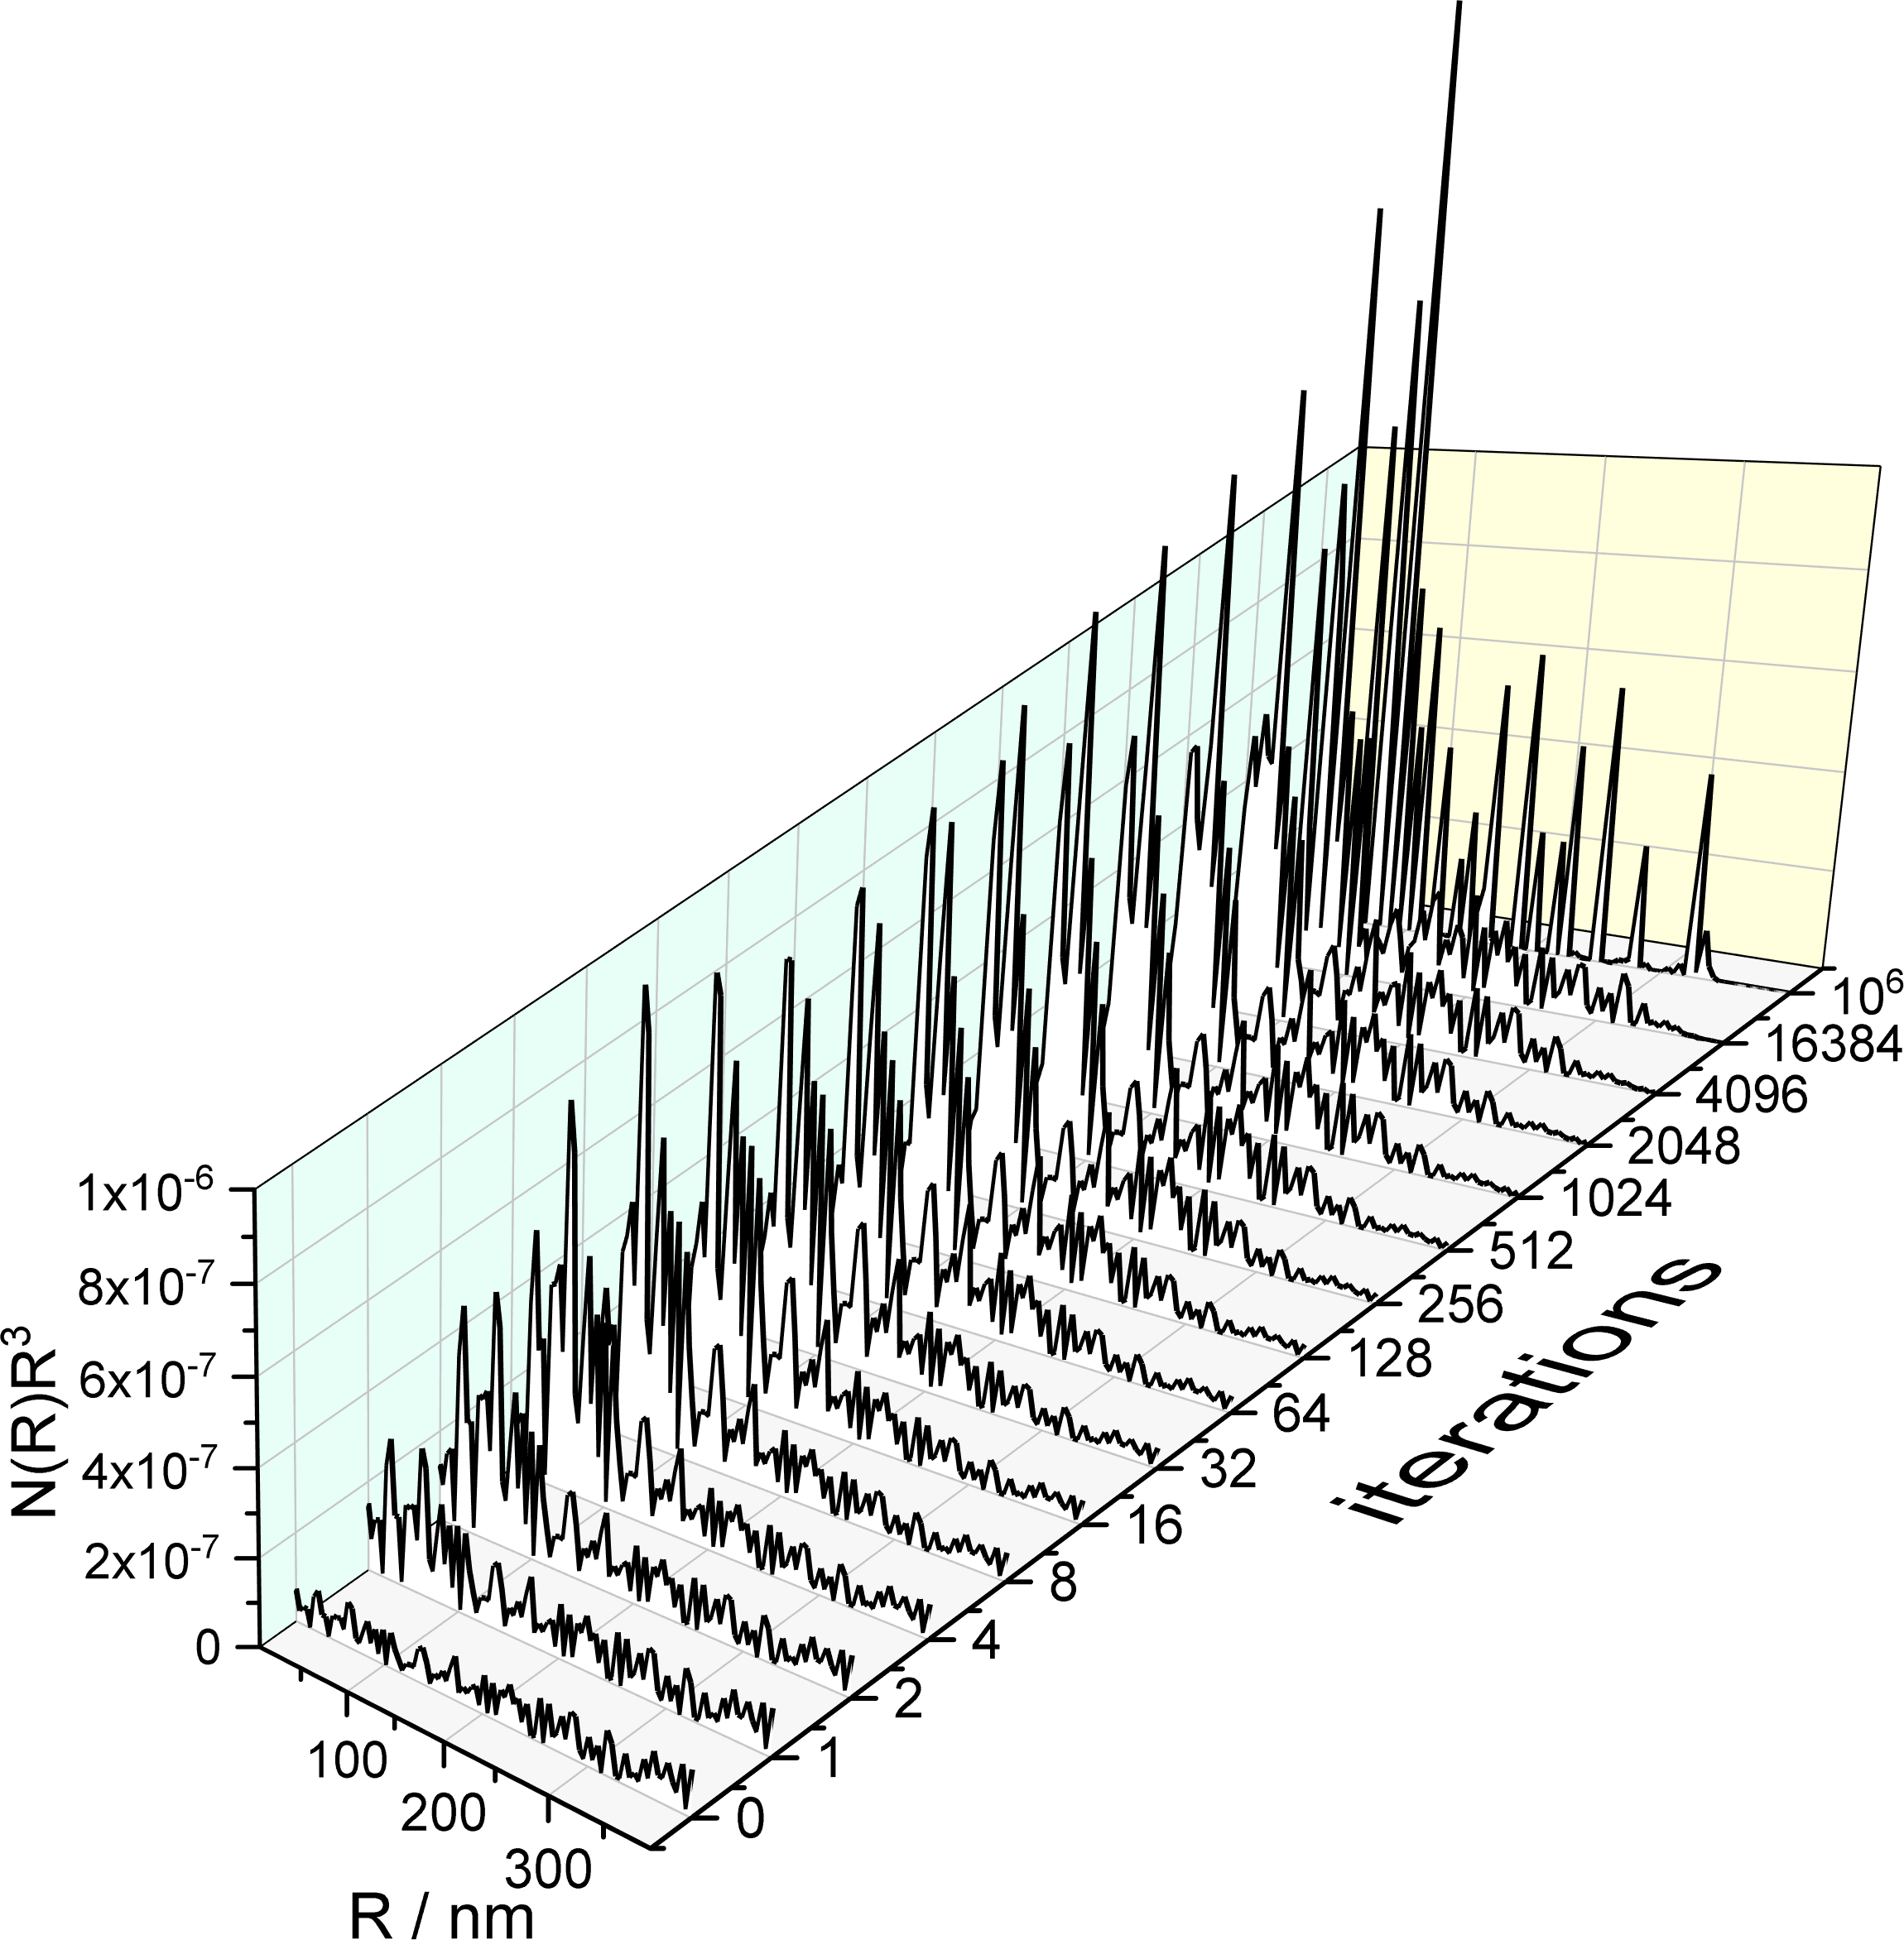
\includegraphics[width=0.46\textwidth]{../images/form_factor/EM/EMrandom_seed_smooth_0_0_NR.png}
\caption{Size distribution evolution for increasing number of iterations for a constant seed value (left) and random seed values (right).\label{fig:EMNRevolution}}
\end{figure}

In figure \ref{fig:EMIQevolution} and \ref{fig:EMNRevolution} the progress of the EM-fixed point algorithm as a function of the number of iteration steps is shown. The starting values of the size distribution are assumed to be a constant (left) and random (right). In both cases the EM-scheme converges in that example finally to the same solution. However, assuming constant initial values the size distribution looks relatively smooth until the goodness-of-fit parameter approaches its final value in contrast to random seed values for the size distribution, where the initial roughness is never smoothed out by the EM scheme. In figure \ref{fig:EMgoodness_smooth_evolution} the goodness-of-fit parameters are shown as a function of iterations. For this three variants of the goodness-of-fit definitions are used, the classical $\chi_r^2$ of reduced weighted sums of squared  residuals, the $\mathcal{G}$-test which is directly related to the Kubler-Leibler divergency of two probability function and the Pearson's $\chi_P^2$-test, which is obtained by a second order Taylor expansion of the natural logarithm around 1 of the  $\mathcal{G}$-test.
\begin{align}
  \chi_r^2 &= \sum_i^N \frac{1}{N}\left(\frac{I_\mathrm{th}(q_i)-I_\mathrm{exp}(q_i)}{\Delta I_\mathrm{exp}(q_i)}\right)^2 &~ &\mbox{weighted sum of squared residuals} \label{eq:goodnessoffit_chi2}\\
  \chi_P^2 &= \sum_i \frac{\left(I_\mathrm{th}(q_i)-I_\mathrm{exp}(q_i)\right)^2}{I_\mathrm{th}(q_i)} &~ &\mbox{Pearson's $\chi^2$-test} \label{eq:goodnessoffit_chi2test}\\
  \mathcal{G} &= 2\sum_i \mathcal{I}_\mathrm{exp}(q_i)\ln\left(\frac{\mathcal{I}_\mathrm{exp}(q_i)}{\mathcal{I}_\mathrm{th}(q_i)}\right) &~ & \mathcal{G}\mbox{-test} \label{eq:goodnessoffit_Gtest}
\end{align}
with $\mathcal{I}_\mathrm{exp}(q_i)=I_\mathrm{exp}(q_i)/\sum_i I_\mathrm{exp}(q_i)$ and $\mathcal{I}_\mathrm{th}(q_i)=I_\mathrm{th}(q_i)/\sum_i I_\mathrm{th}(q_i)$.
Furthermore the roughness of the resulting size distribution is plotted which has been described by either the sum of the squared first or second derivatives for all radii, i.e. $\sum_i \abs{\mathrm{d}N(R_i)/\mathrm{d}R_i}^2$ or $\sum_i \abs{\mathrm{d}^2N(R_i)/\mathrm{d}R_i^2}^2$.
\begin{figure}[htb]
\centering
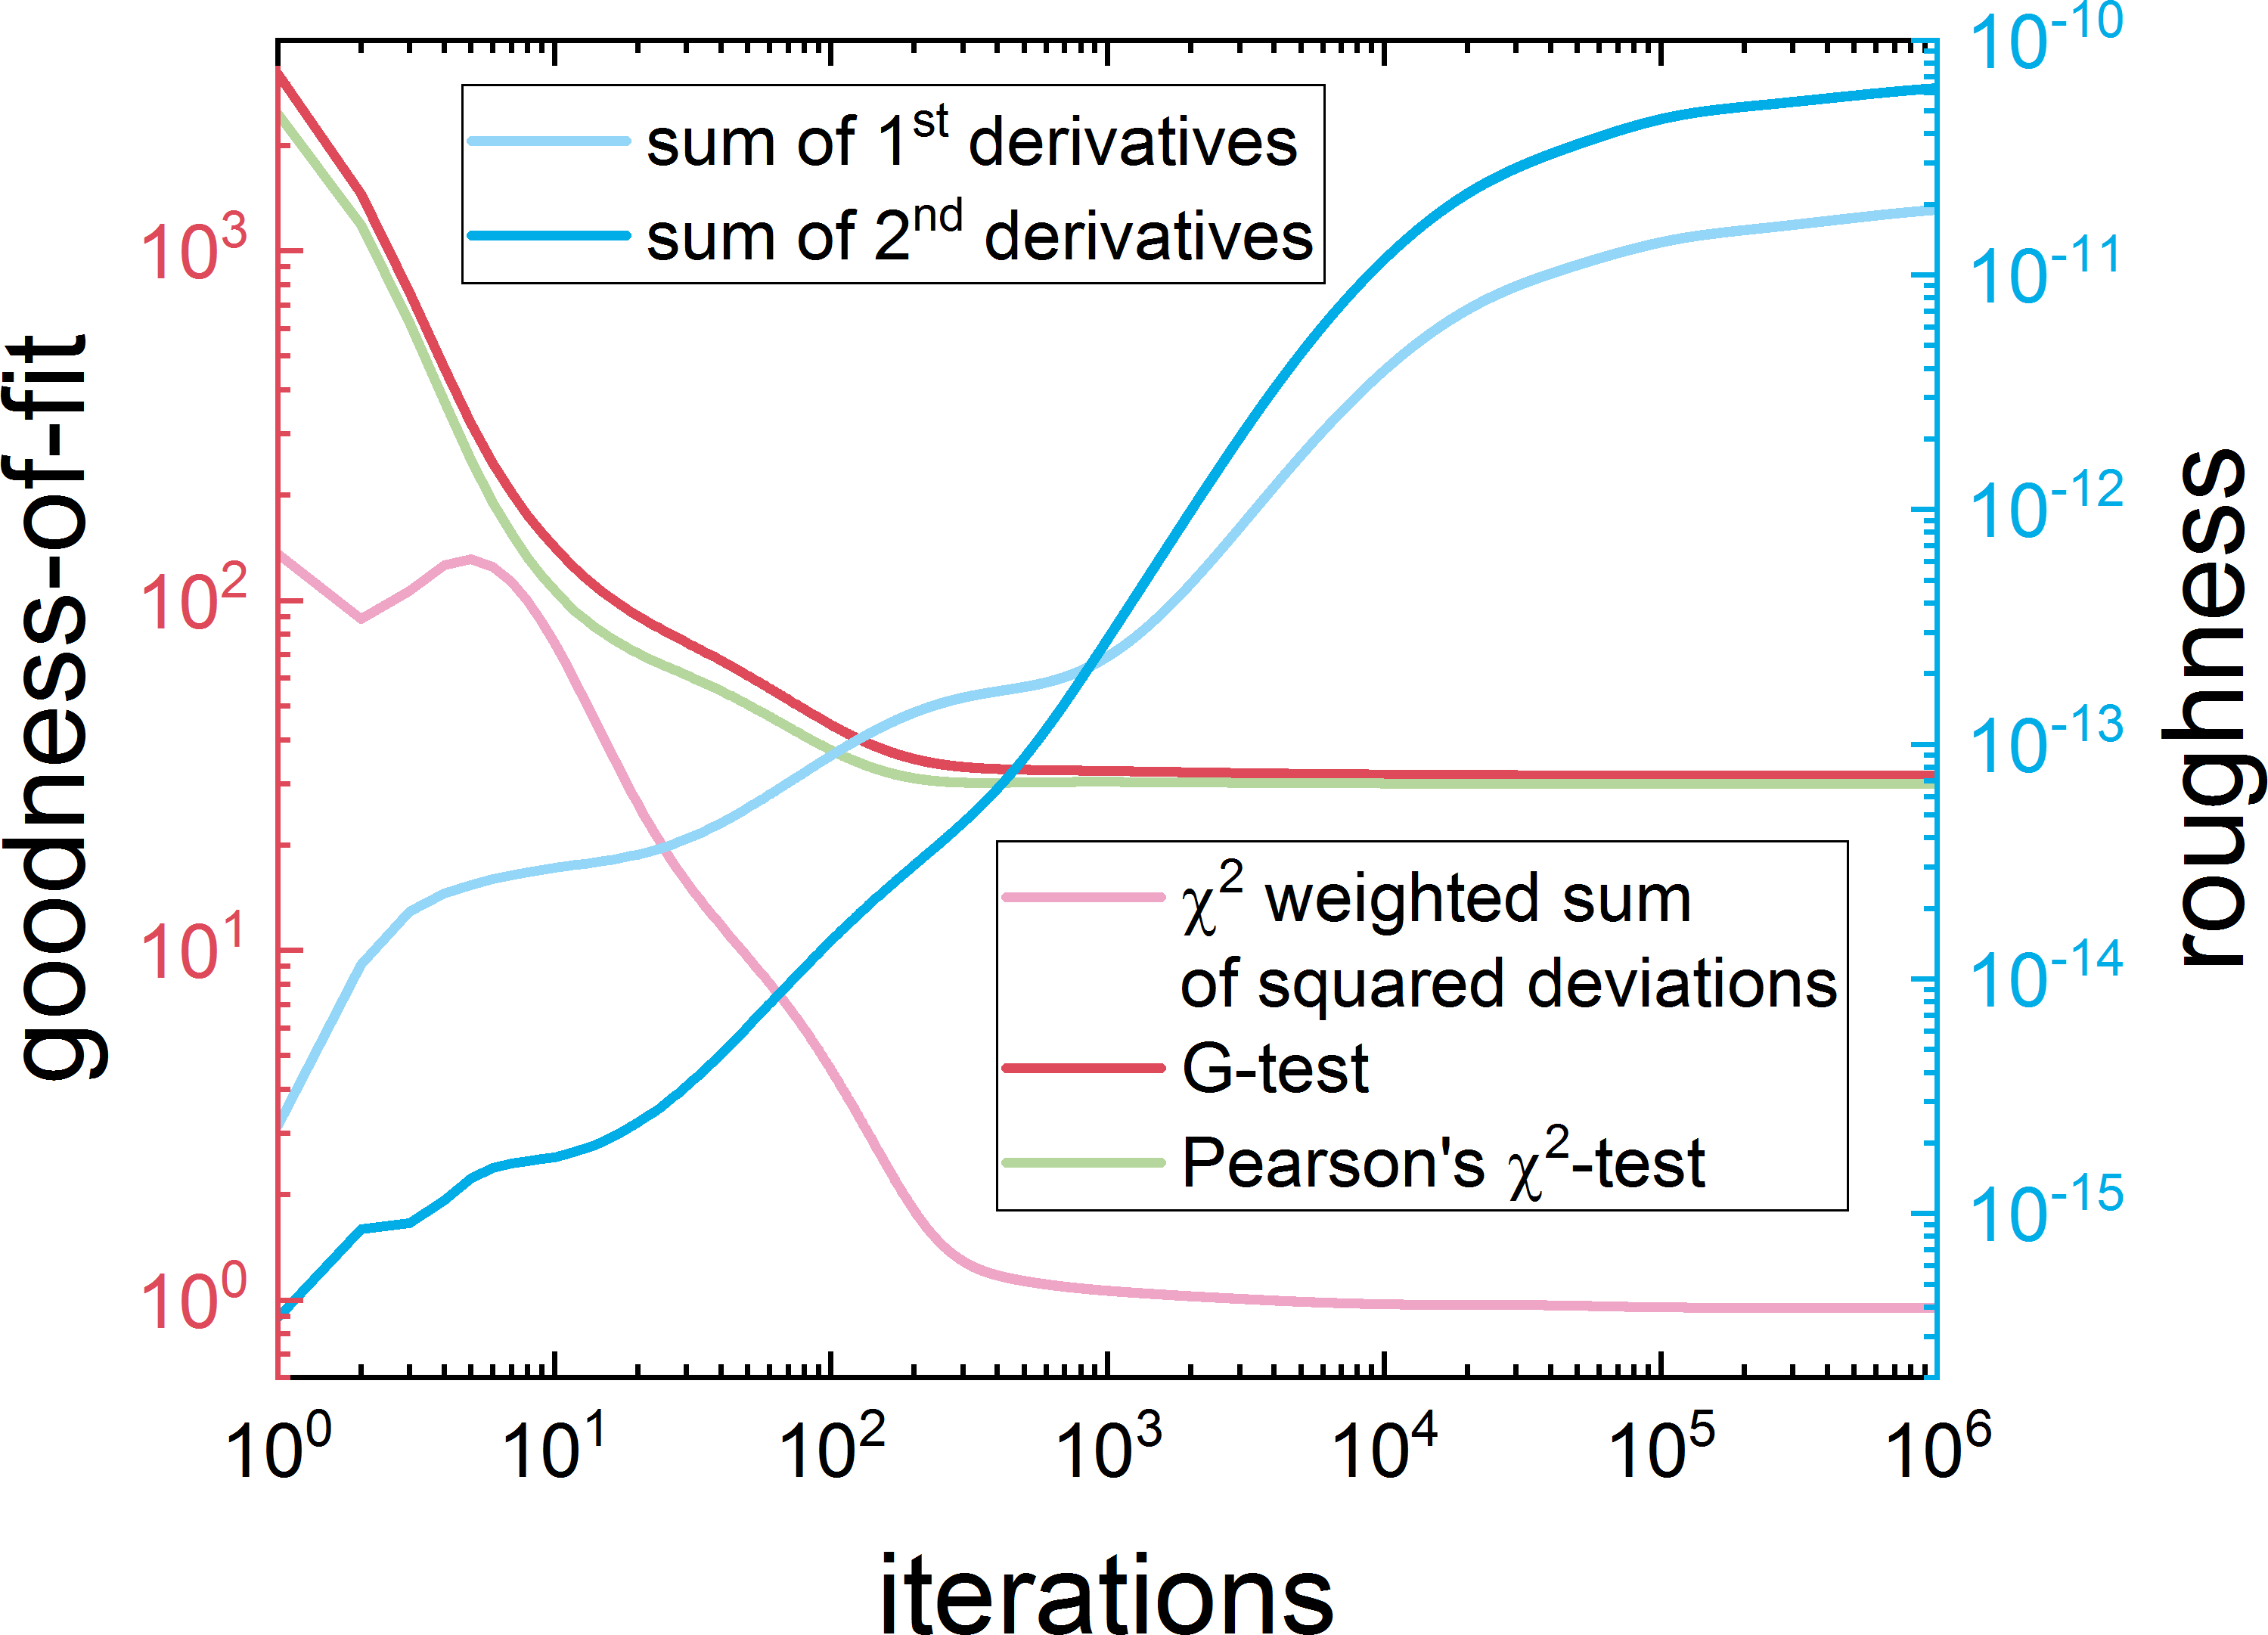
\includegraphics[width=0.46\textwidth]{../images/form_factor/EM/EMconstant_seed_smooth_0_0_goodness_of_fit.png}
\hspace{0.06\textwidth}
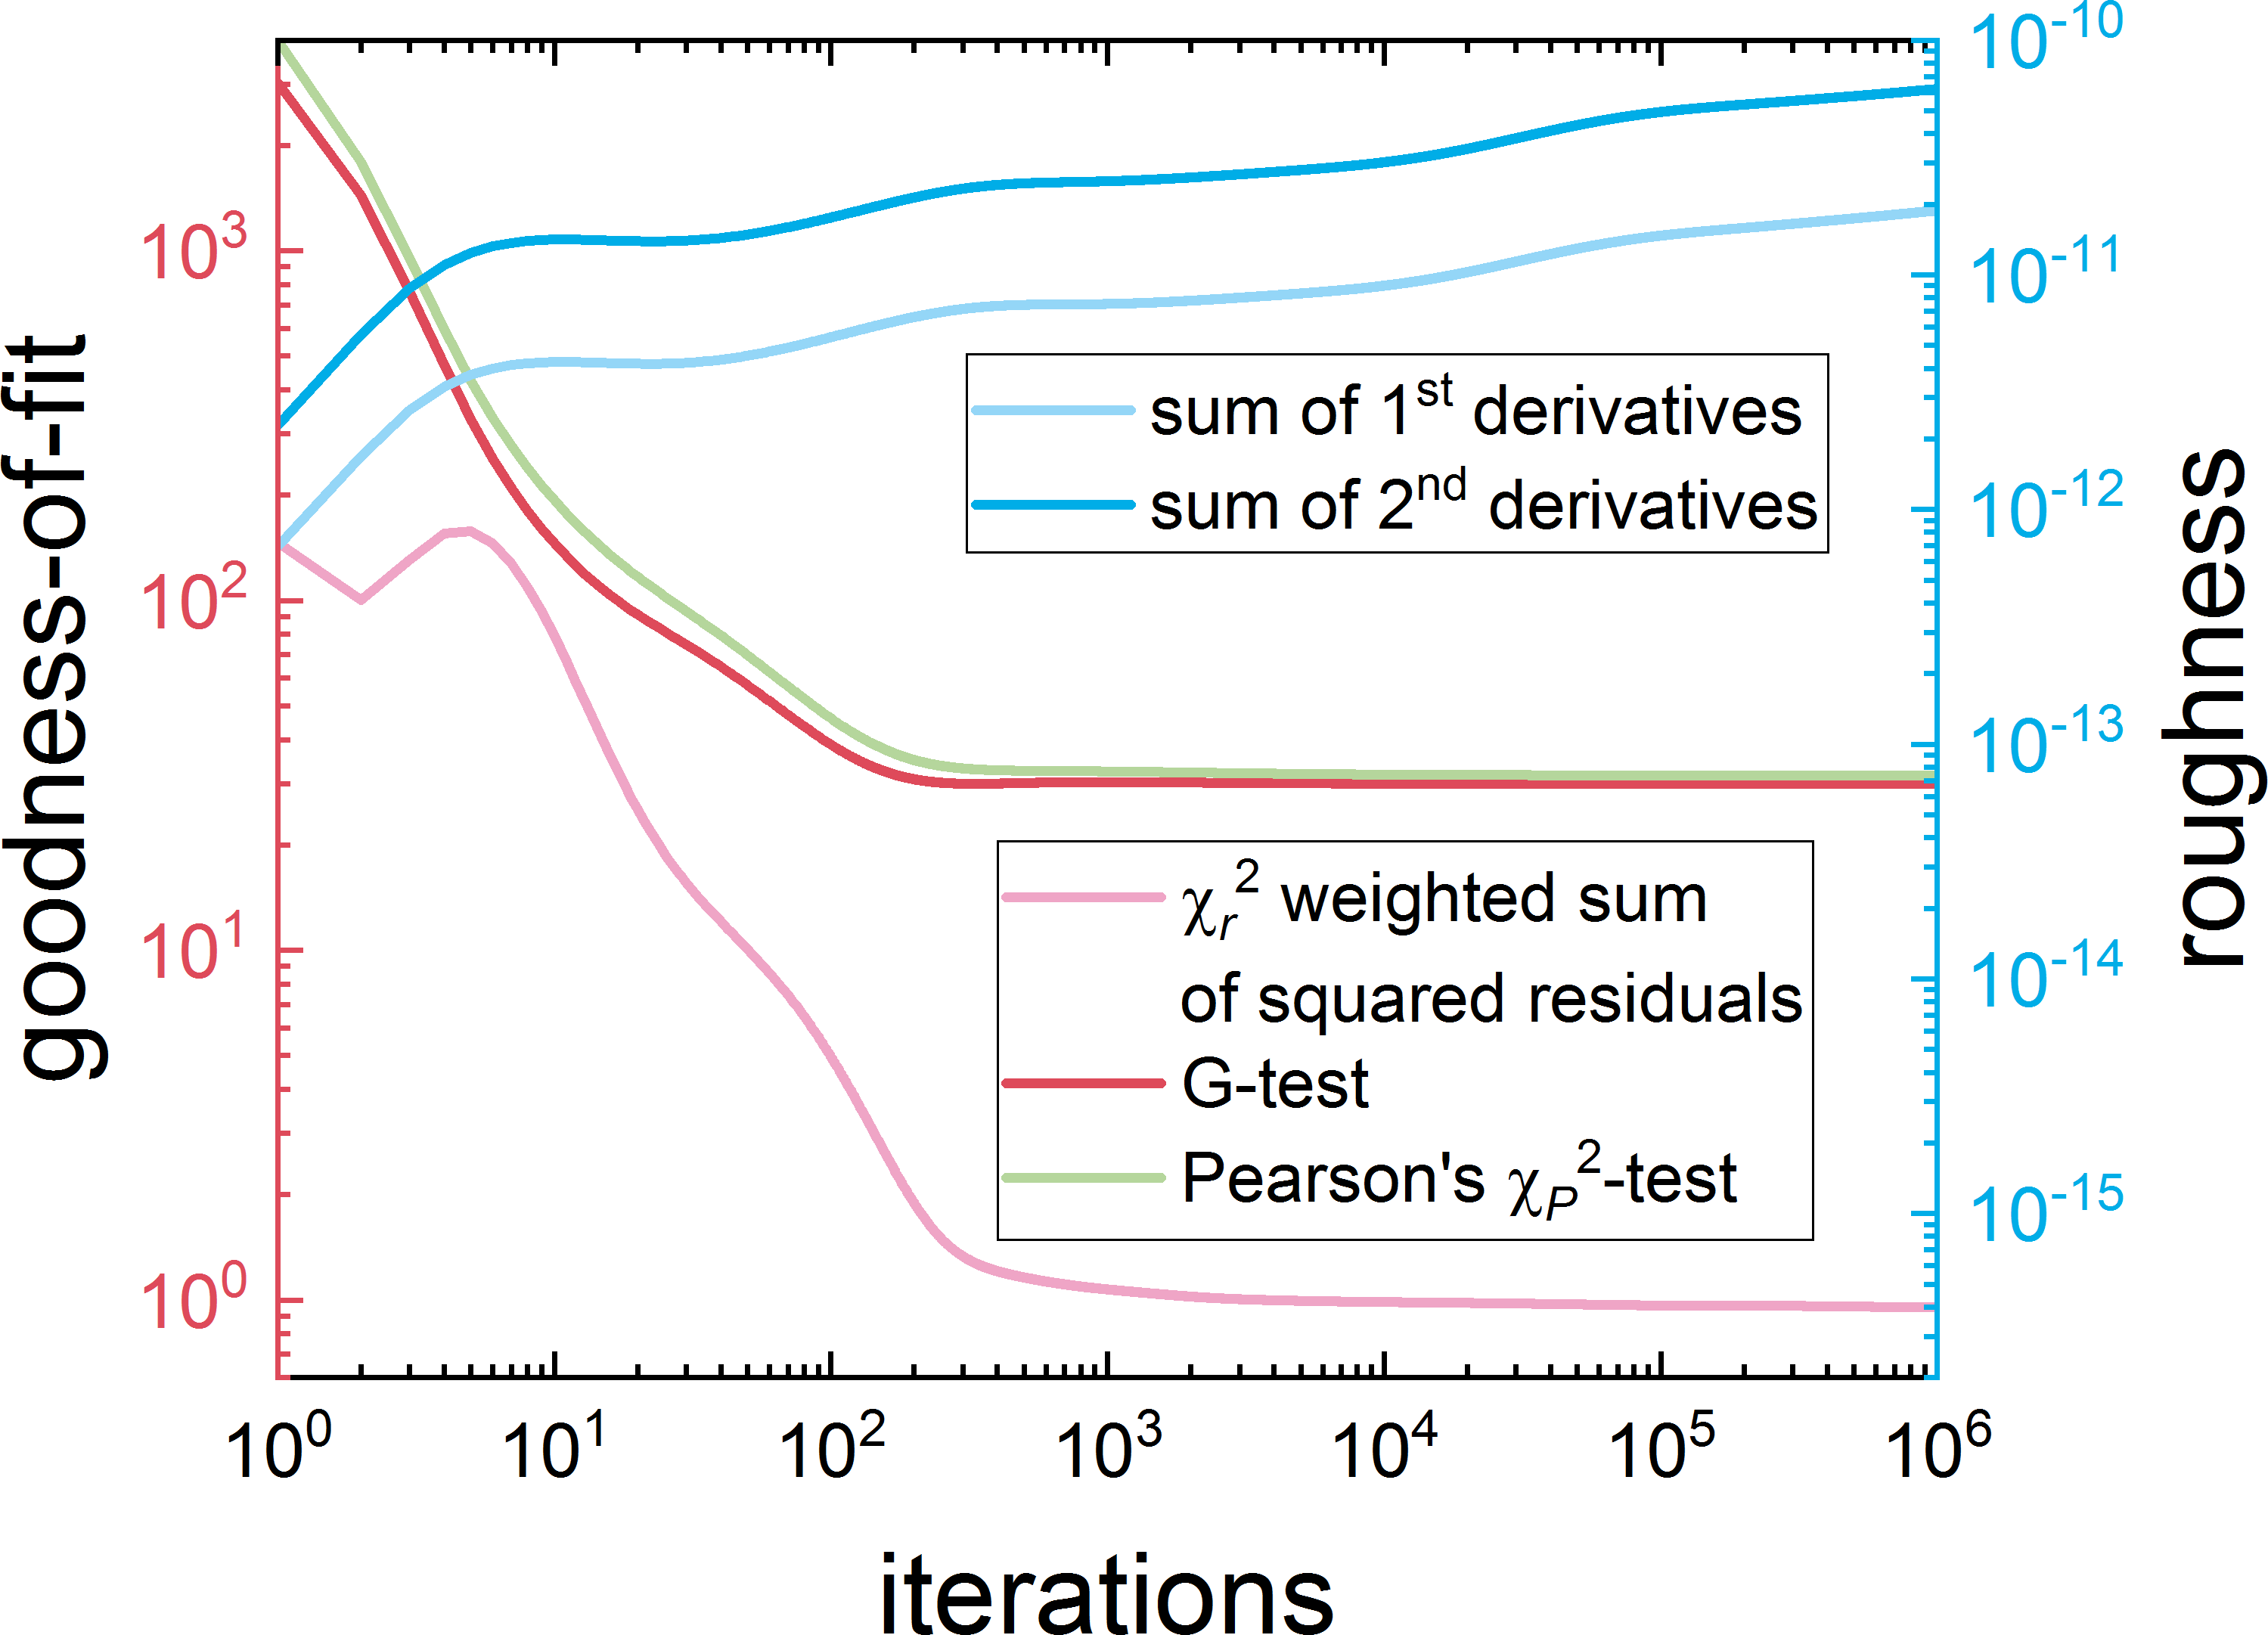
\includegraphics[width=0.46\textwidth]{../images/form_factor/EM/EMrandom_seed_smooth_0_0_goodness_of_fit.png}
\caption{Dependency of goodness-of-fit and roughness on number of iterations for a constant seed value (left) and random seed values (right).\label{fig:EMgoodness_smooth_evolution}}
\end{figure}

The roughness parameter and the goodness-of-fit parameter are then combined in figure \ref{fig:EMLcurves} on loglog-scale showing somehow a similar behaviour as the L-curve in regularization techniques solving ill-posed problems. From a certain number of iterations the goodness-of-fit only improves infinitesimal but the roughness still continuous for a quite large number of iterations before it reaches the fixed point.

\begin{figure}[htb]
\centering
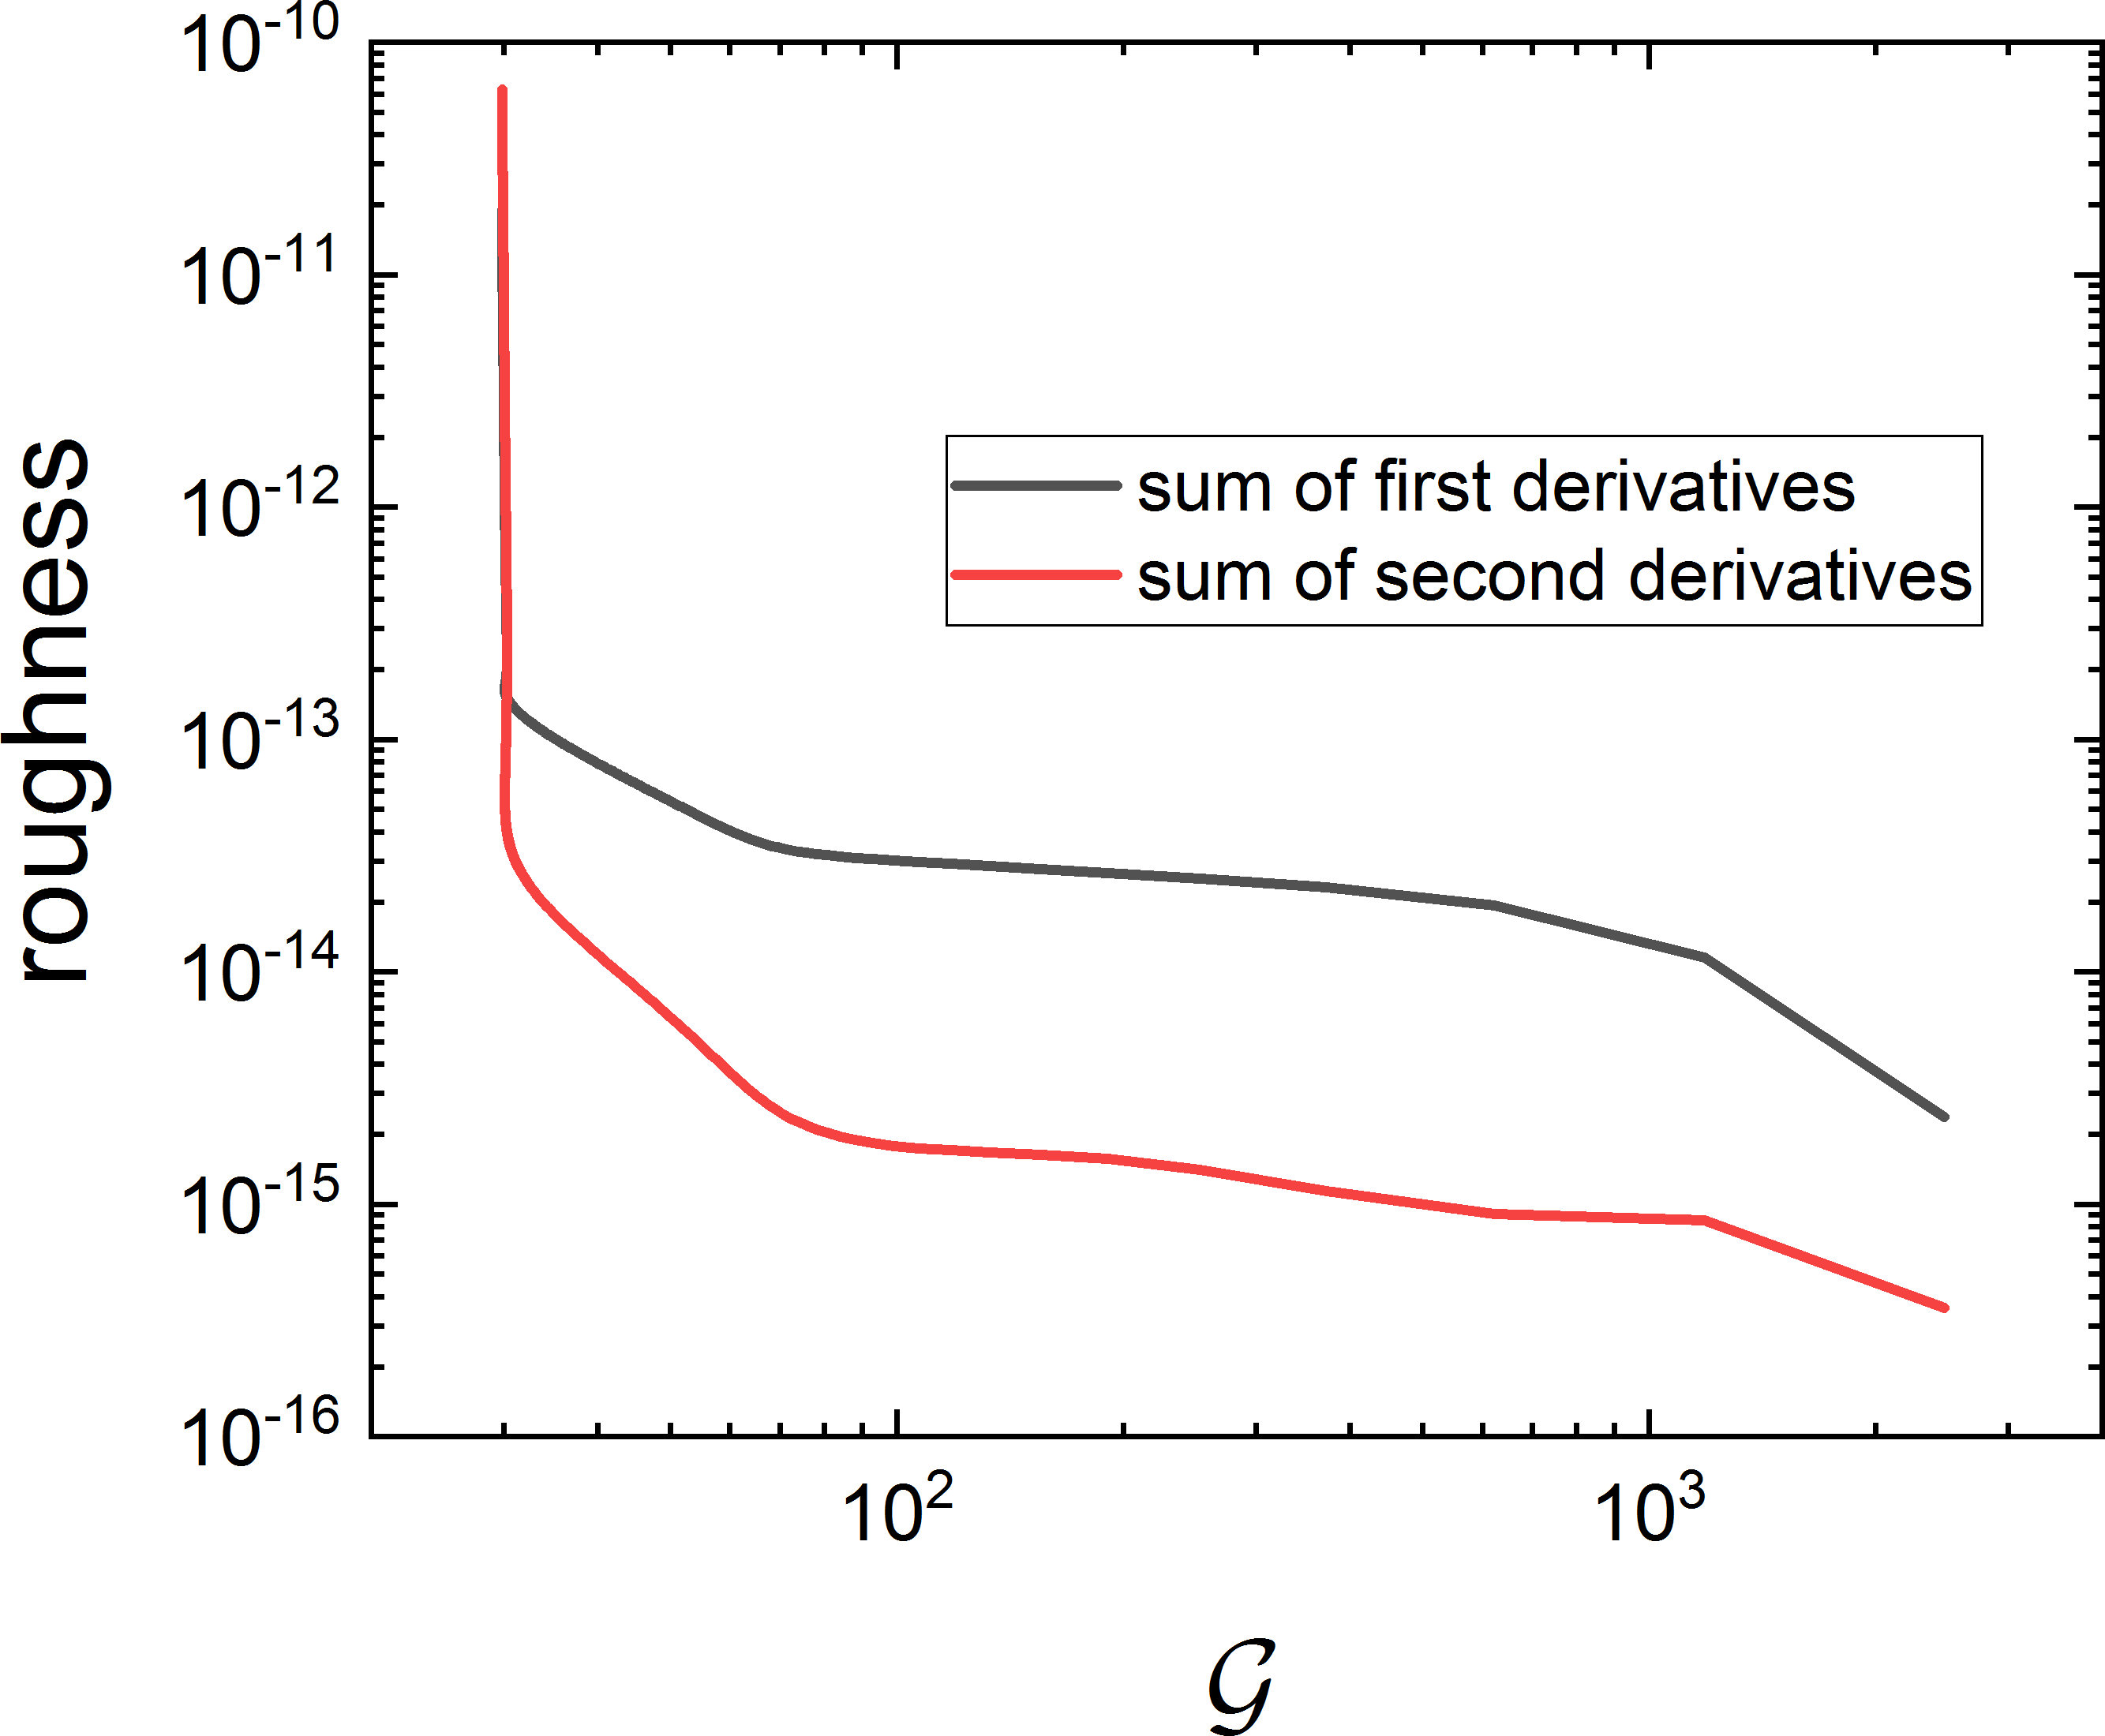
\includegraphics[width=0.44\textwidth]{../images/form_factor/EM/EMconstant_seed_smooth_0_0_L_curve.png}
\hspace{0.1\textwidth}
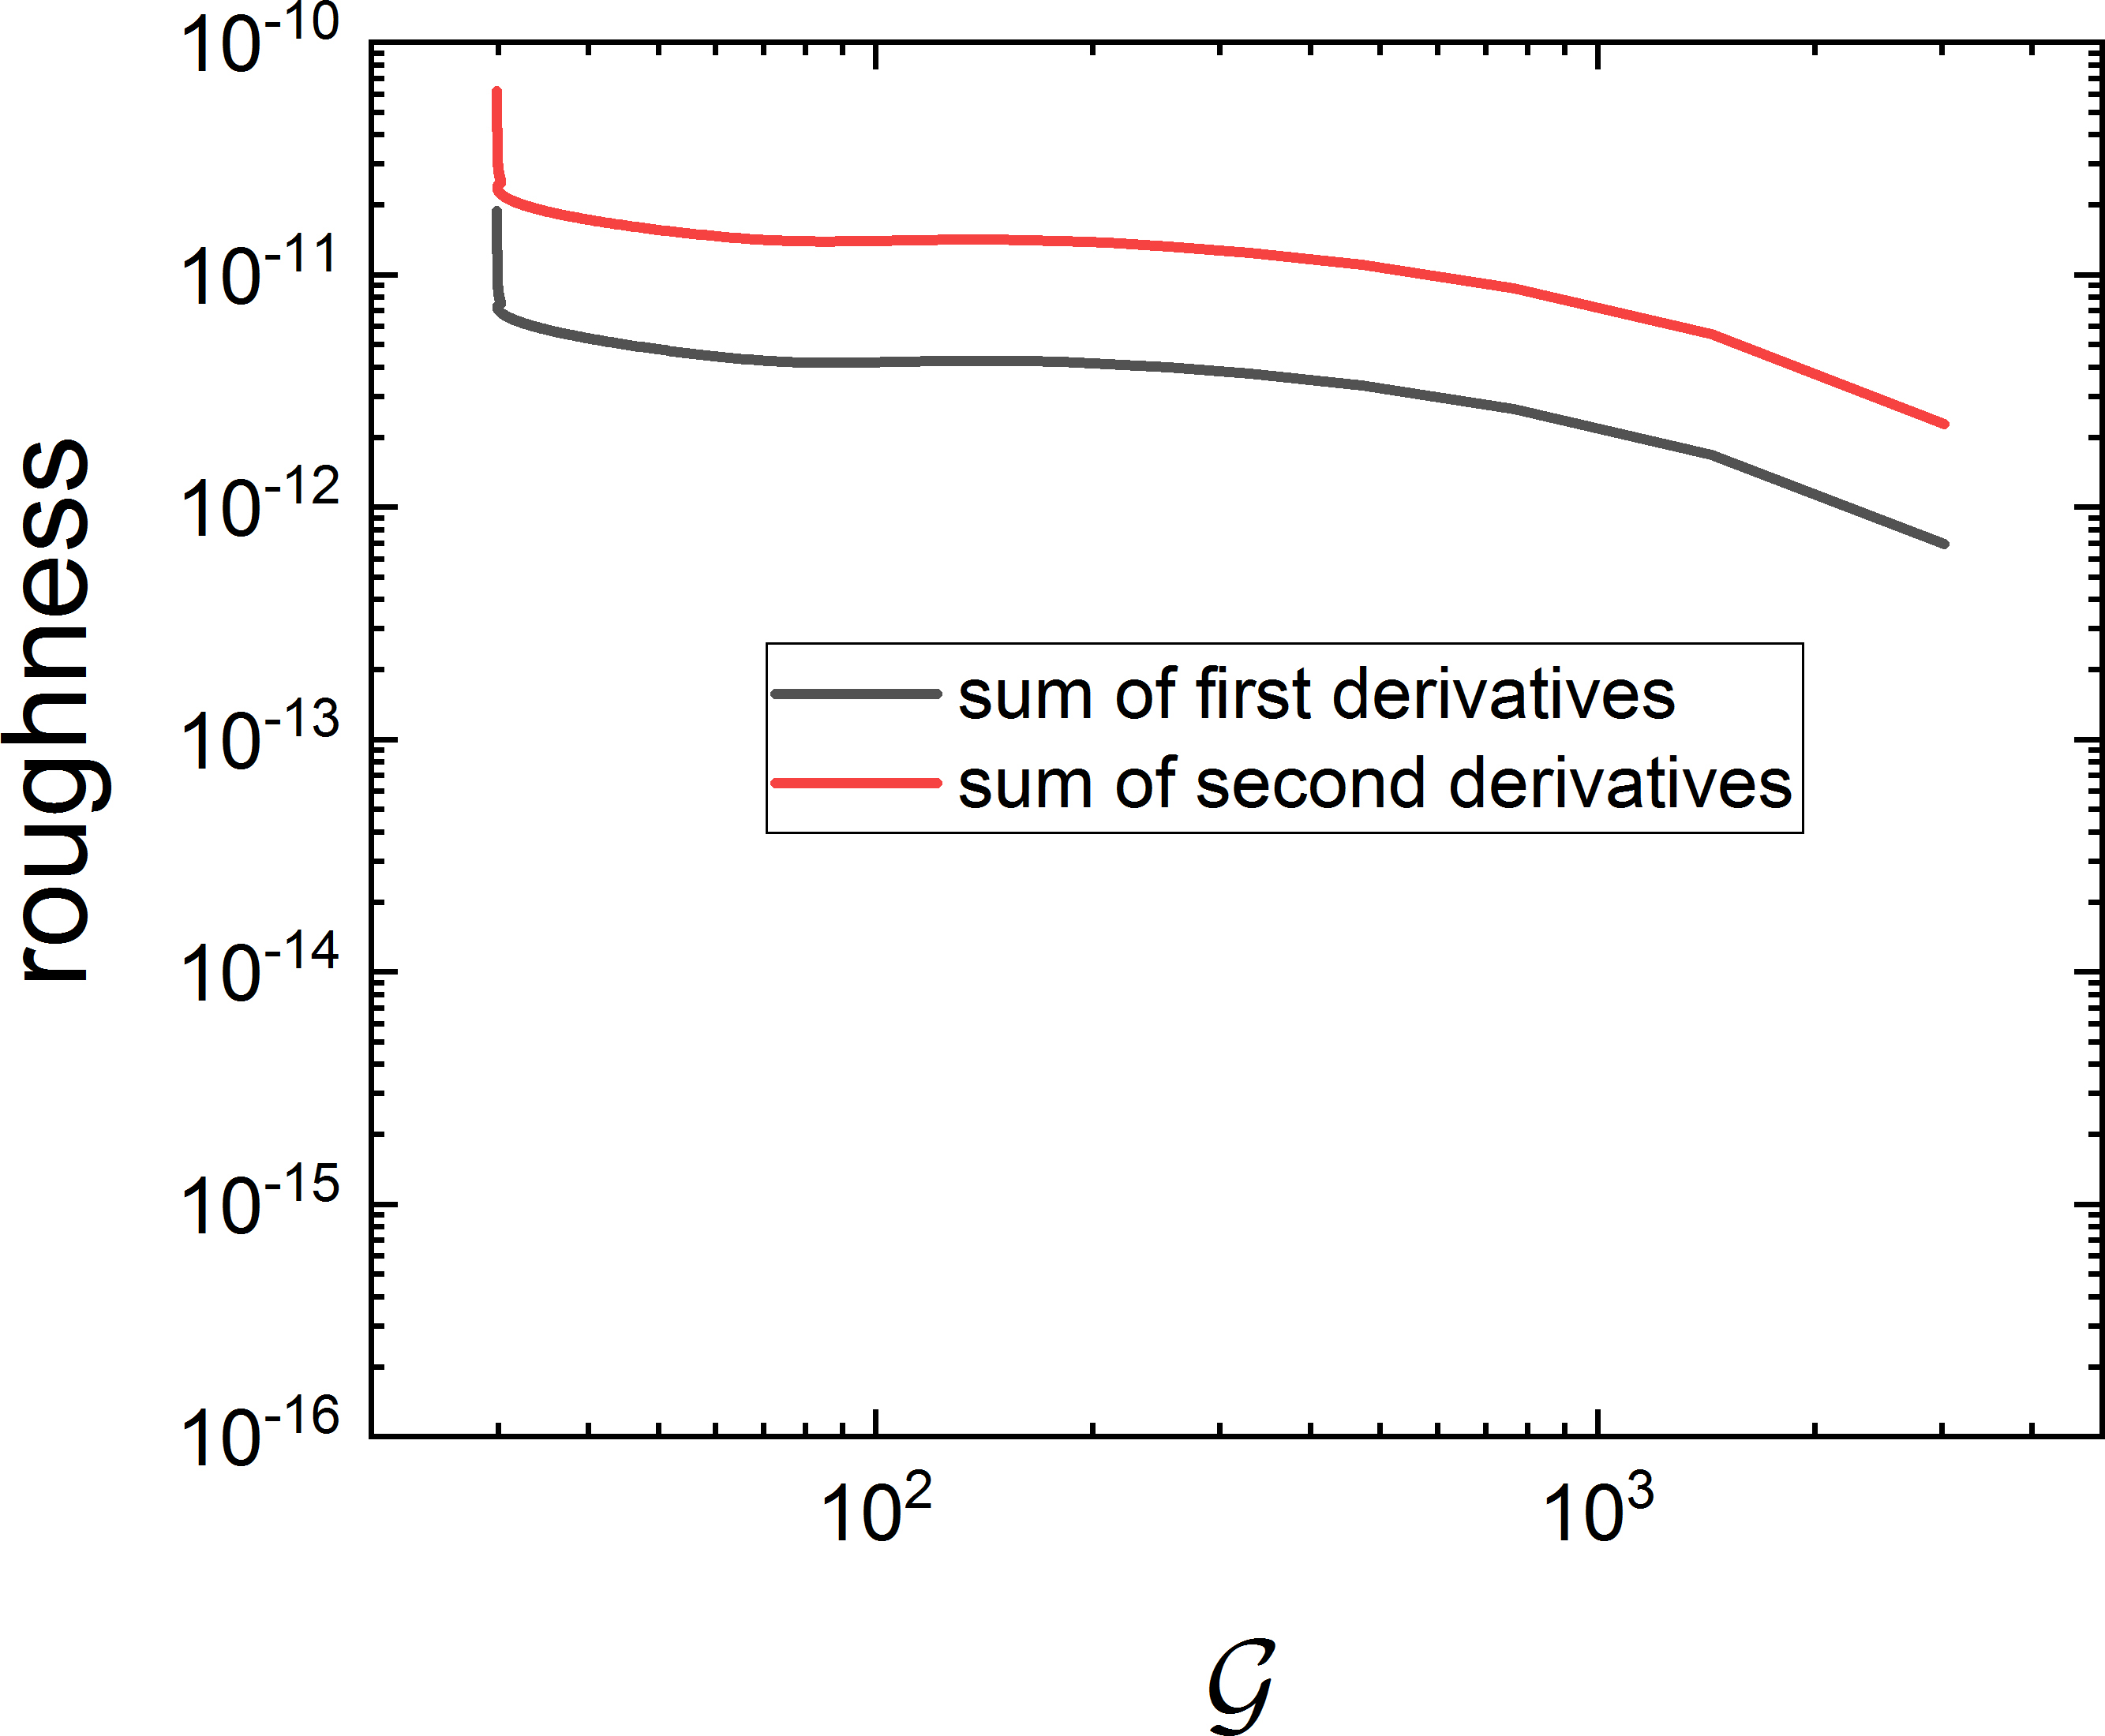
\includegraphics[width=0.44\textwidth]{../images/form_factor/EM/EMrandom_seed_smooth_0_0_L_curve.png}
\caption{L-curve showing the dependency of the roughness parameters on the goodness-of-fit parameters for a constant seed value (left) and random seed values (right).\label{fig:EMLcurves}}
\end{figure}

Even though the fixed point of the EM operator does not seem to depend on the initialization of the starting values but it will probably depend on the actual noise on the data, i.e. if the curve would be measured a second time with similar statistics the two curves would differ within their noise level and the EM fixed point would then very likely be slightly different, which is caused by the ill-posed nature of the Fredholm integral. Two strategies for overcoming this problem has been tested. One strategy introducing a smoothing operator into the iteration loop and a second strategy to introduce a classical regularization term in the EM scheme, which both then require a determination of the smoothing or regularization parameter.

~\\

\subsection{EM with linear and non-linear smoothing operator}~\\

 Without any additional smoothing the EM scheme does not converge to a stable solution for scattering curves measured several times with the same statistics. Several stabilization methods have been suggested. One of them is to add an additional smoothing operator into the iteration sequence. In \SASfit the smoothing operation  suggested by \cite{Eggermont1999,Eggermont1995,Byrne2011} has been implemented. They suggest to add before or/and after each normal EM step (eq.\ \ref{eq:LucyRichardsonInversionMethod}) an additional smoothing step so that the EM algorithm takes the form.
\begin{align}\label{eq:smoothedEMsingle}
  x_j^{(k+1/2)} &= x_j^{(k)} + \Delta x_j^{(k)}   \\
  x_j^{(k+1)} &= \displaystyle \sum_{i=0}^{M-1} S^{(h)}_{ij} x_j^{(k+1/2)}
\end{align}
with the smoothing operator
\begin{align}\label{eq:smoothingOperator}
  \hat{\mathbf{S}}^{(h)} &=
  \begin{pmatrix}
    1-h    & h      & 0      & \cdots & 0      & 0 \\
    h      & 1-2h   & h      & \cdots & 0      & 0 \\
    0      & h      & 1-2h   & \cdots & 0      & 0 \\
    \vdots & \vdots & \vdots & \ddots & \vdots & \vdots \\
    0      & 0      & 0      & \cdots & 1-2h   & h \\
    0      & 0      & 0      & \cdots & h      & 1-h
  \end{pmatrix}
\end{align}
whereby $0 < h \lessapprox 0.3$.
In case of a double smoothing they suggested a nonlinear smoothing operator before each EM step so that a complete smoothed EM step reads as
\begin{align}\label{eq:smoothedEMdouble}
  x_j^{(k+1/3)} &= \exp\left(\sum_{i=0}^{M-1} S^{(h)}_{ij} \log\left(x_j^{(k)}\right)\right)\\
  x_j^{(k+2/3)} &= x_j^{(k+1/3)} + \Delta x_j^{(k+1/3)}  \\
  x_j^{(k+1)} &= \displaystyle \sum_{i=0}^{M-1} S^{(h)}_{ij} x_j^{(k+2/3)}
\end{align}

\begin{figure}[htb]
\centering
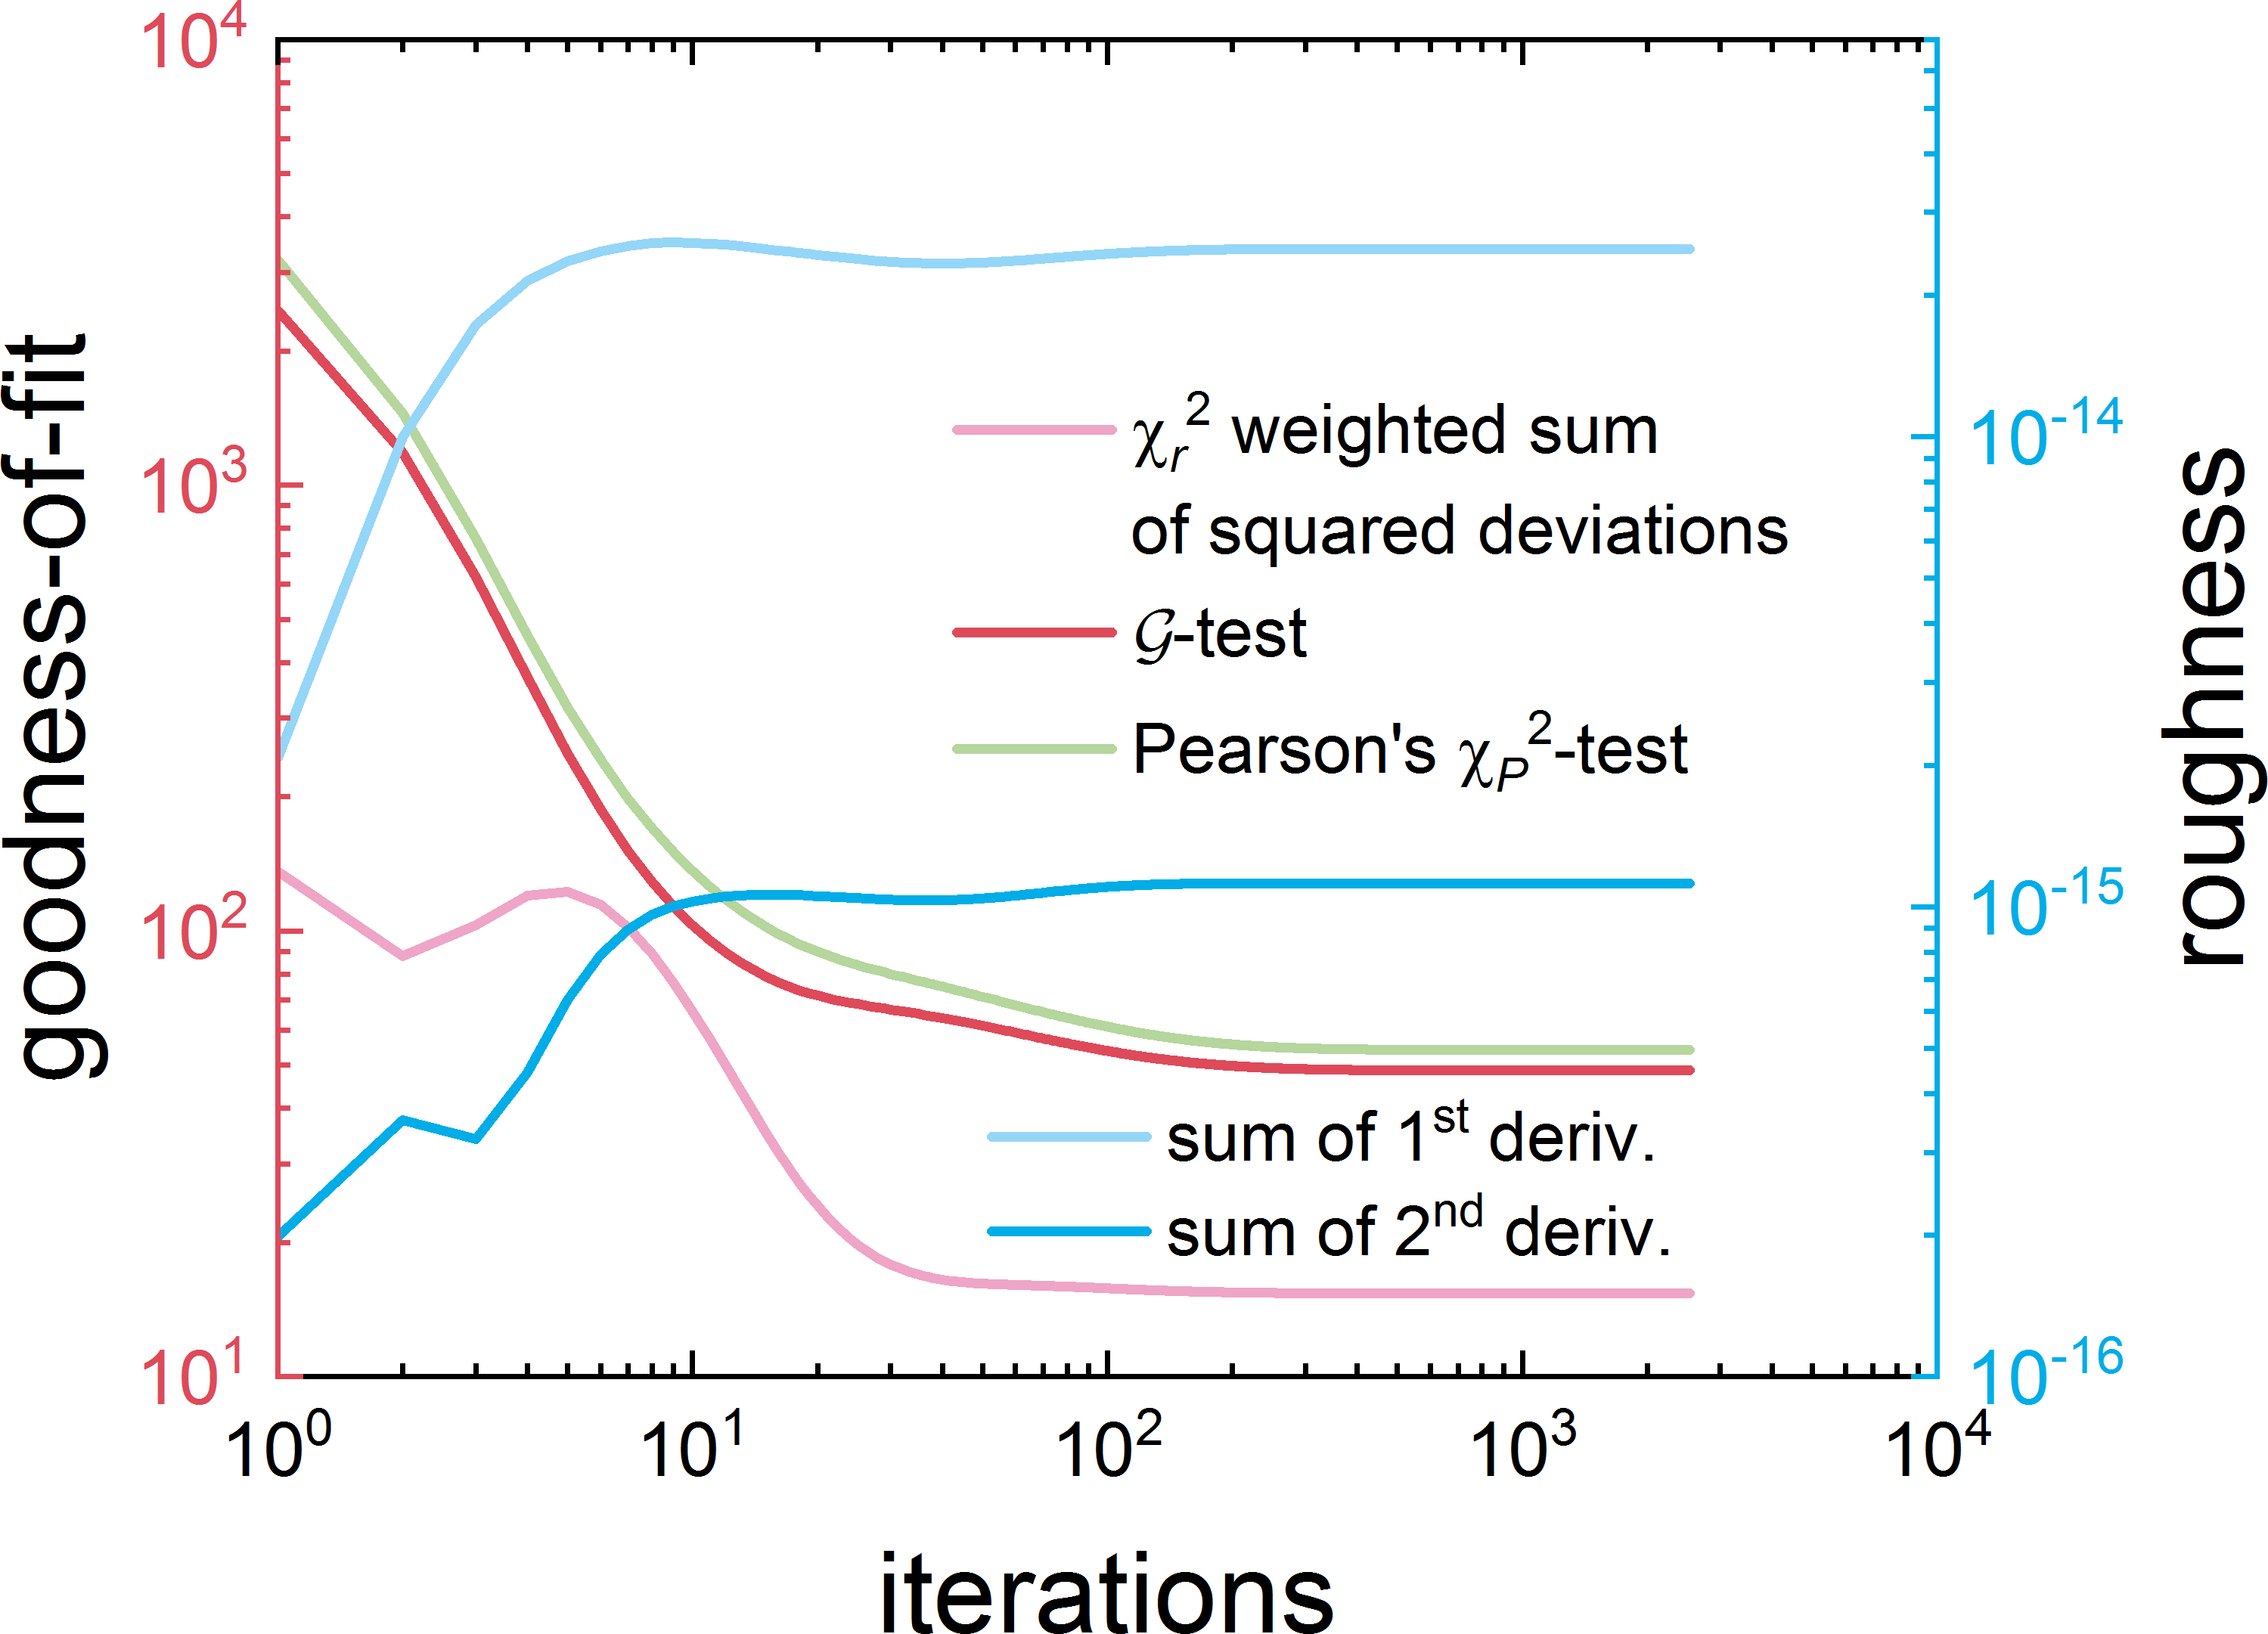
\includegraphics[width=0.48\textwidth]{../images/form_factor/EM/EMconstant_seed_smooth_0_3_goodness_of_fit.png}
\hspace{0.06\textwidth}
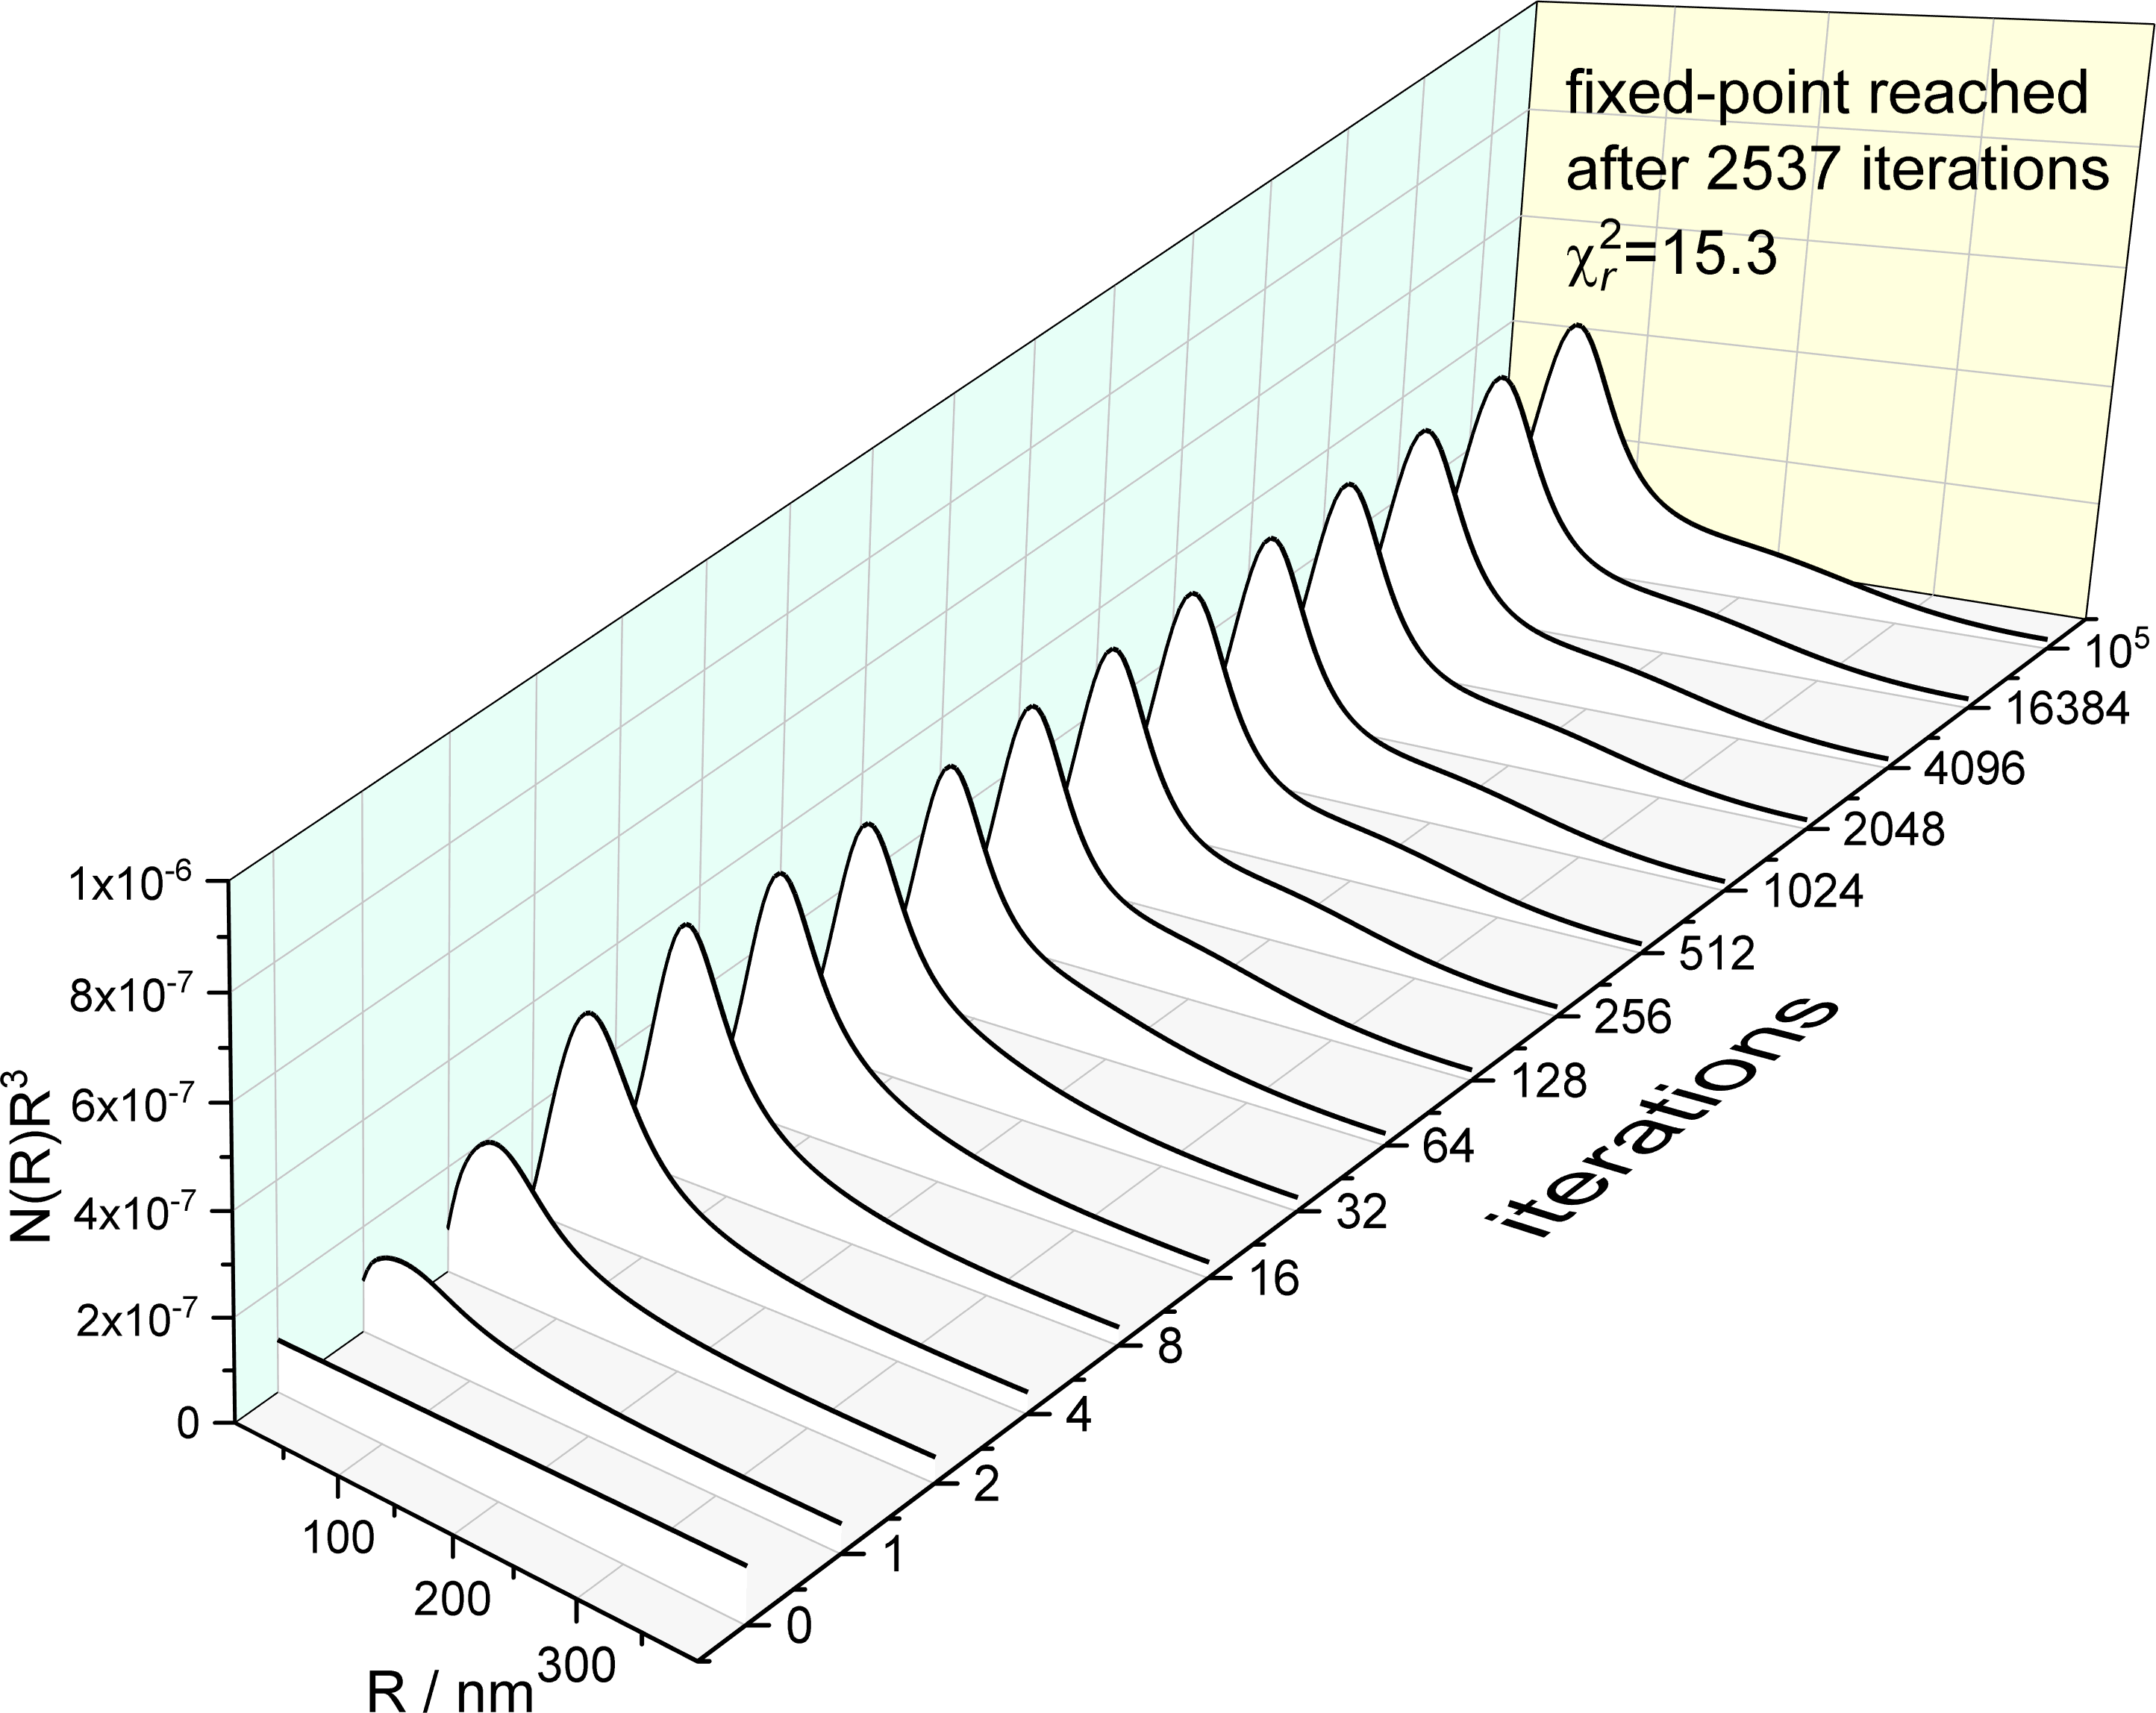
\includegraphics[width=0.42\textwidth]{../images/form_factor/EM/EMconstant_seed_smooth_0_3_NR.png}
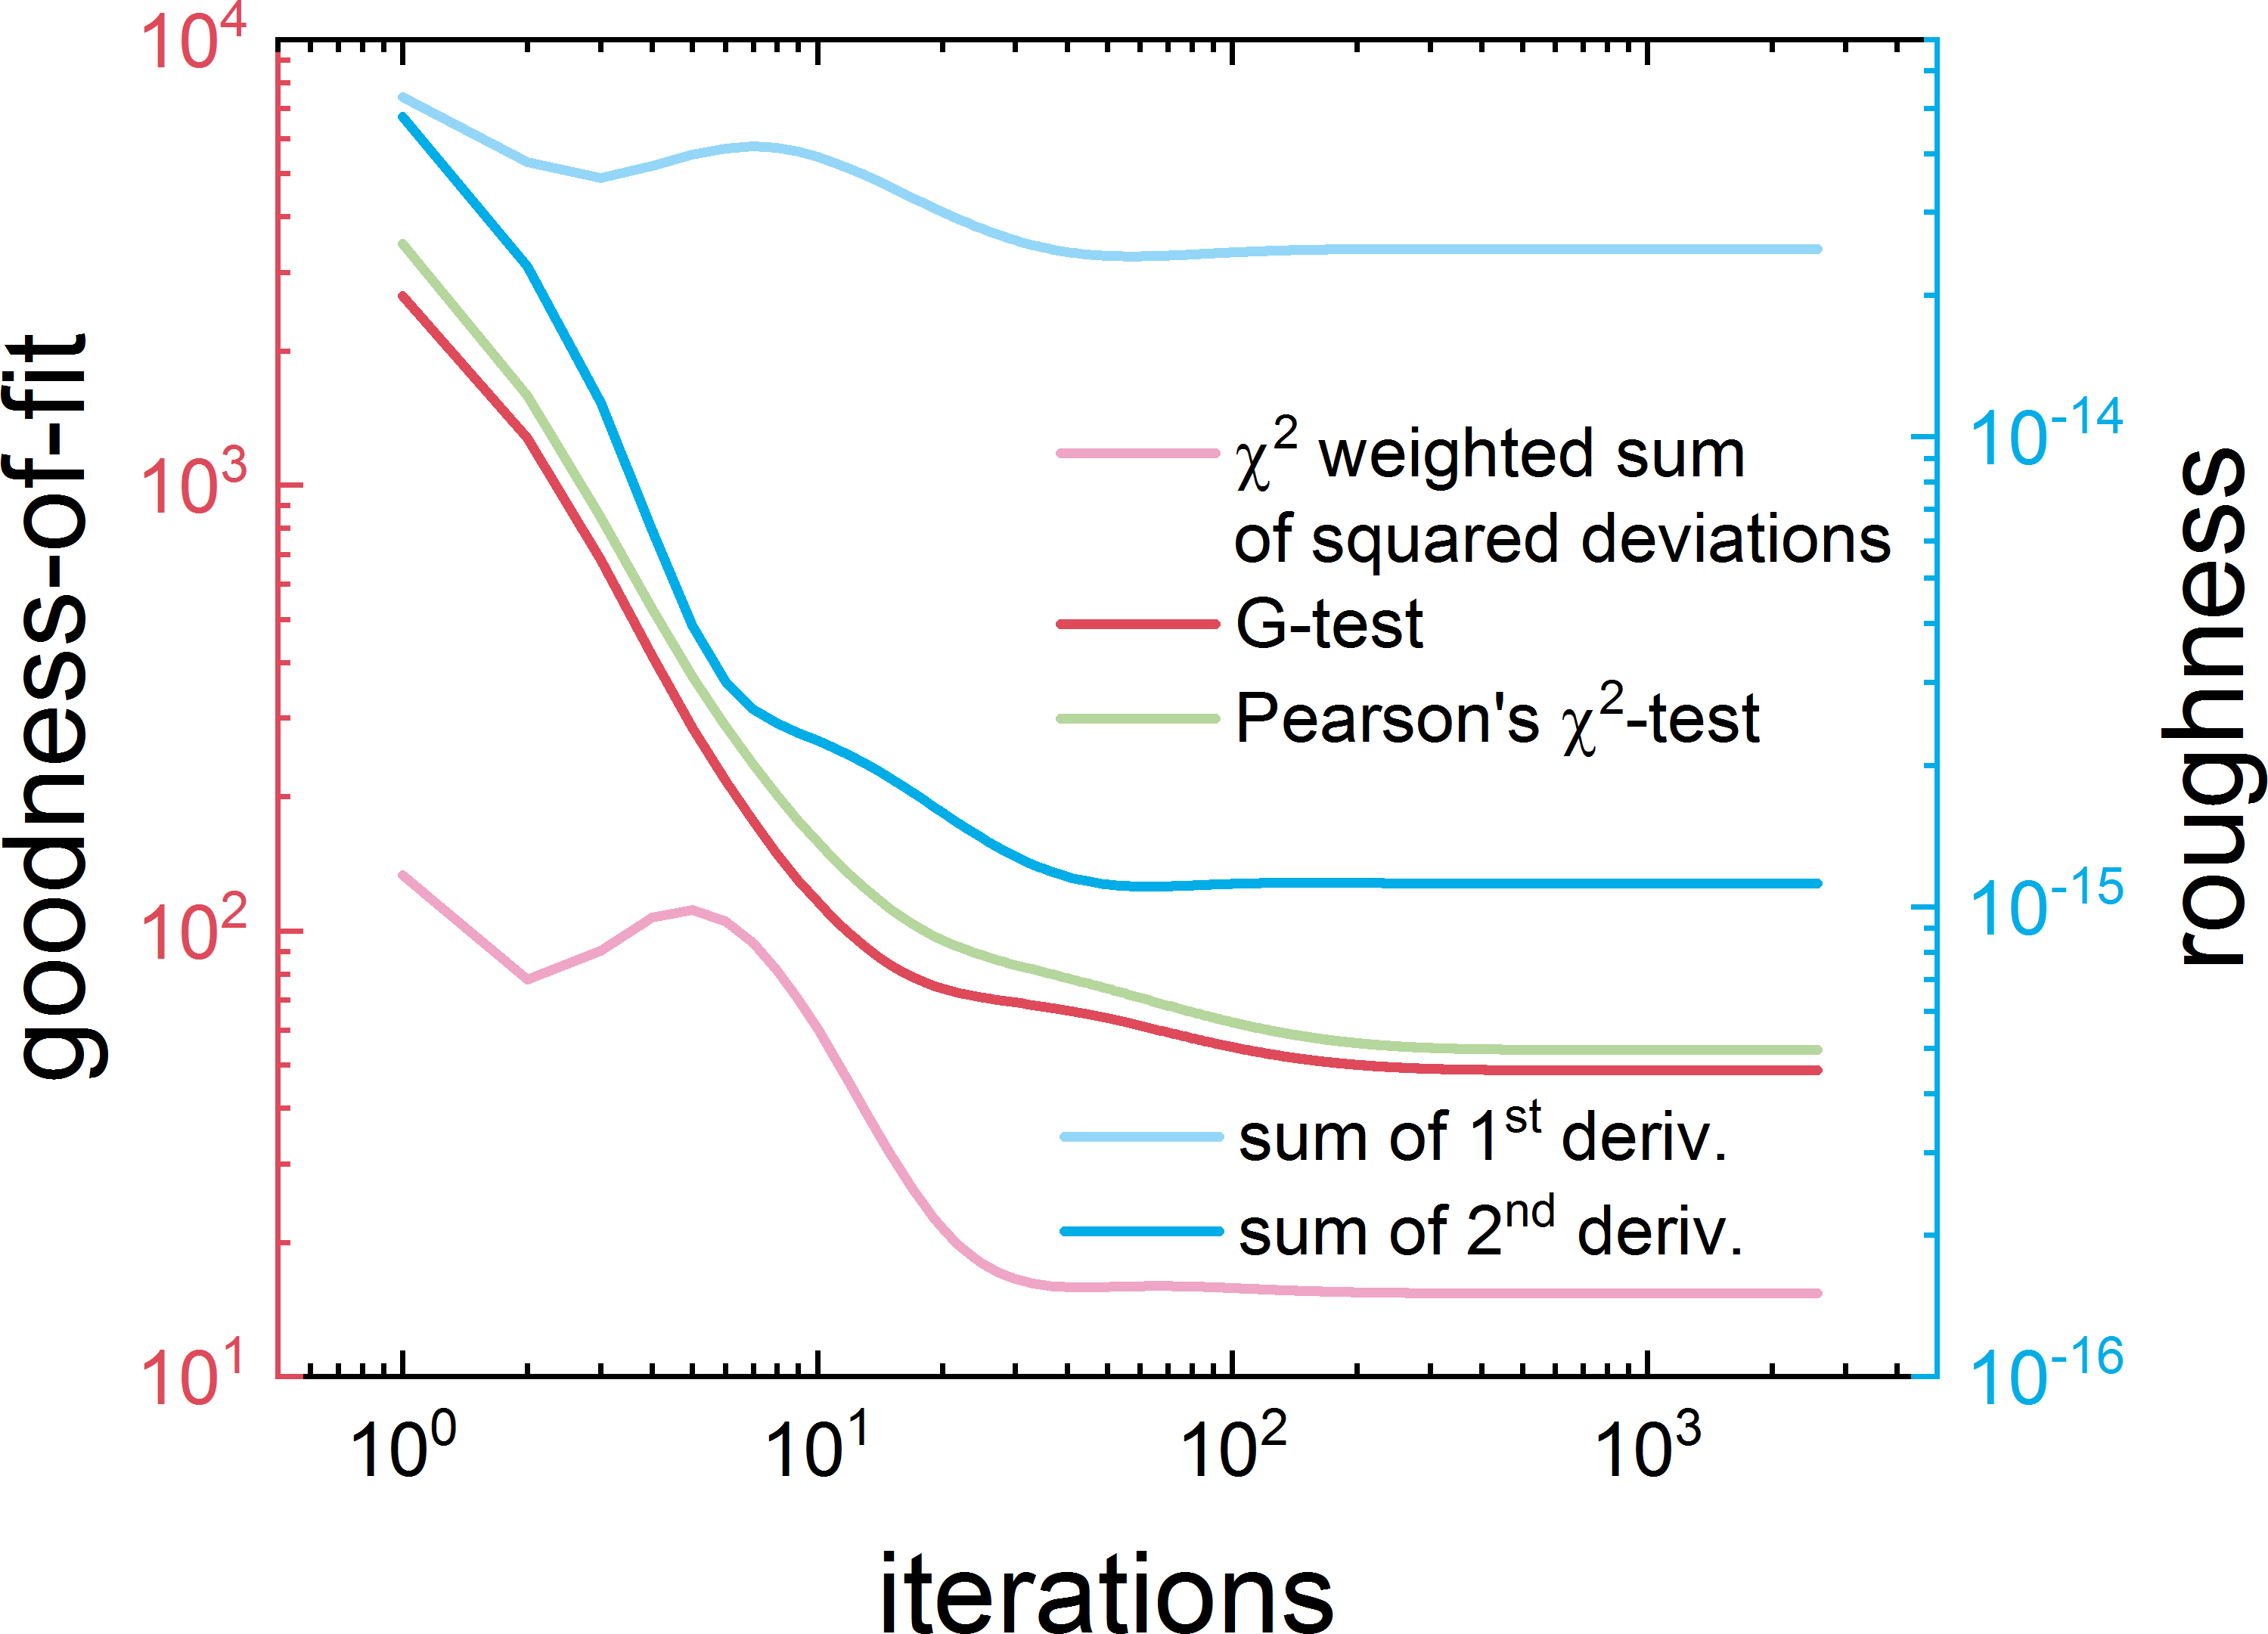
\includegraphics[width=0.48\textwidth]{../images/form_factor/EM/EMrandom_seed_smooth_0_3_goodness_of_fit.png}
\hspace{0.06\textwidth}
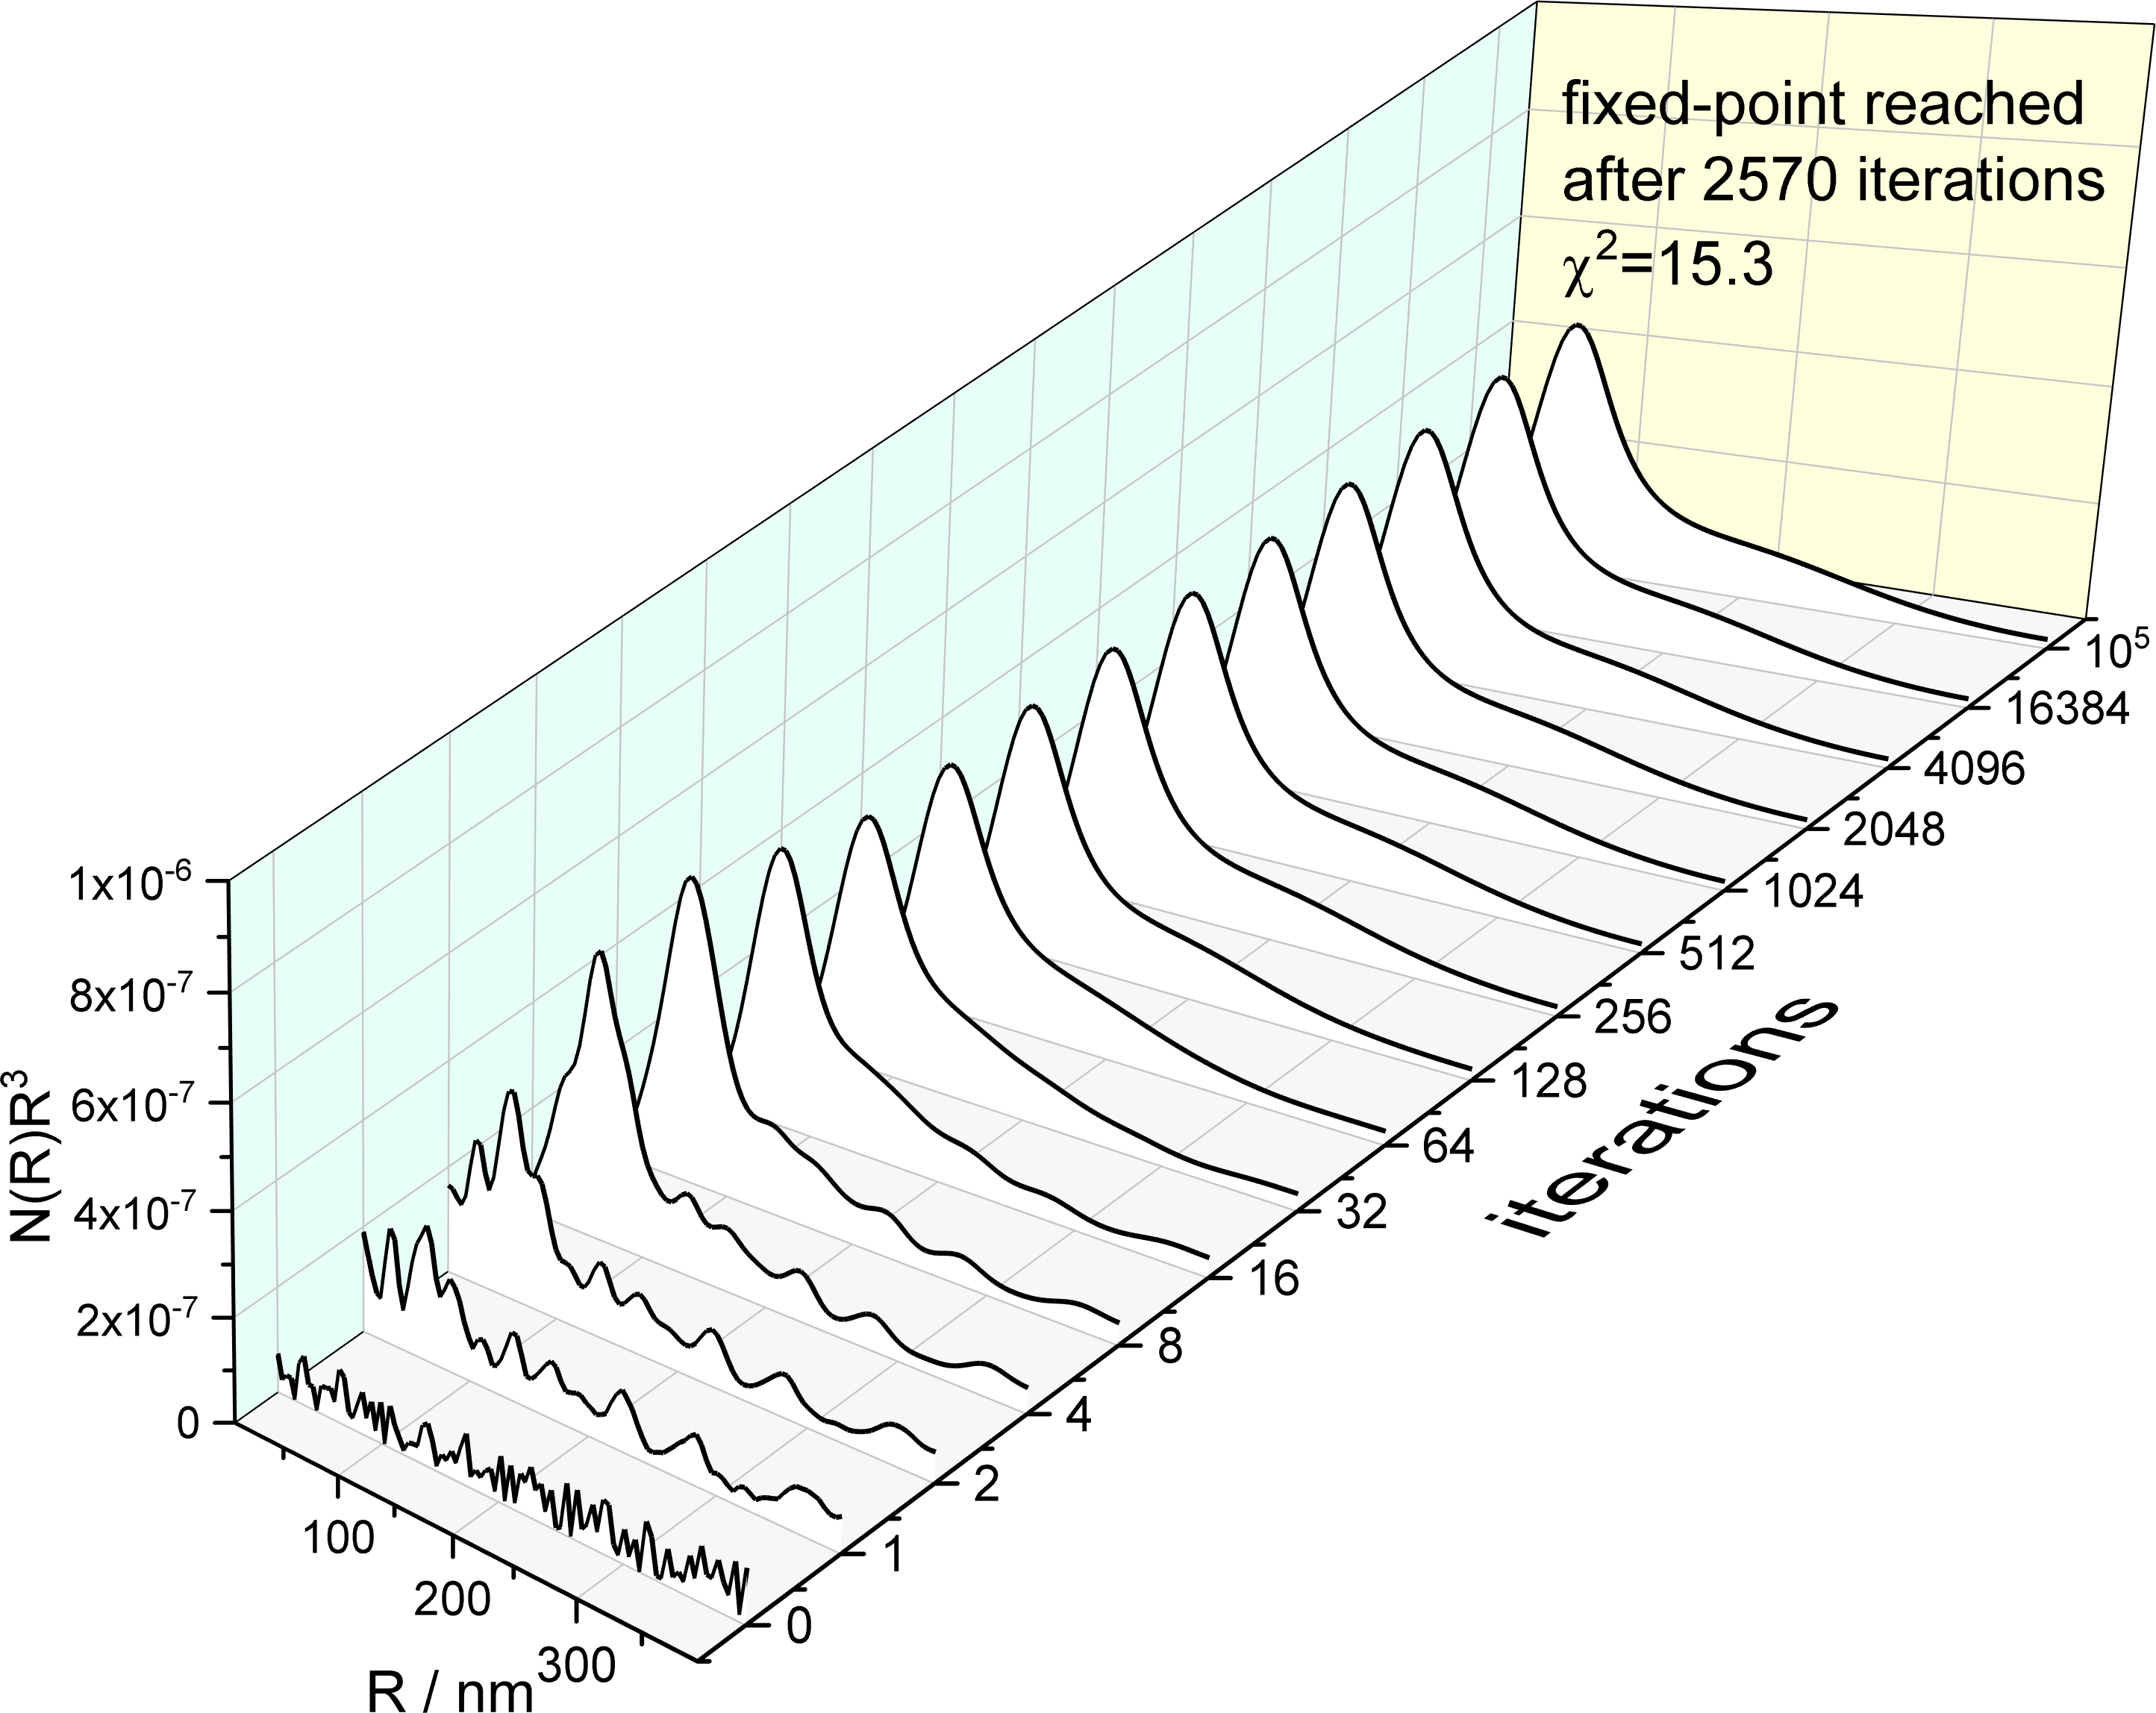
\includegraphics[width=0.42\textwidth]{../images/form_factor/EM/EMrandom_seed_smooth_0_3_NR.png}
\caption{Roughness and goodness-of-fit parameters as well as the resulting volume distribution $N(R)R^3$ as a function of iterations for  a constant seed value (top) and random seed values (bottom) for a large smoothing parameter $h=0.3$ leading to $\chi_r^2=15.3$.\label{fig:EMhlarge}}
\end{figure}

\begin{figure}[htb]
\centering
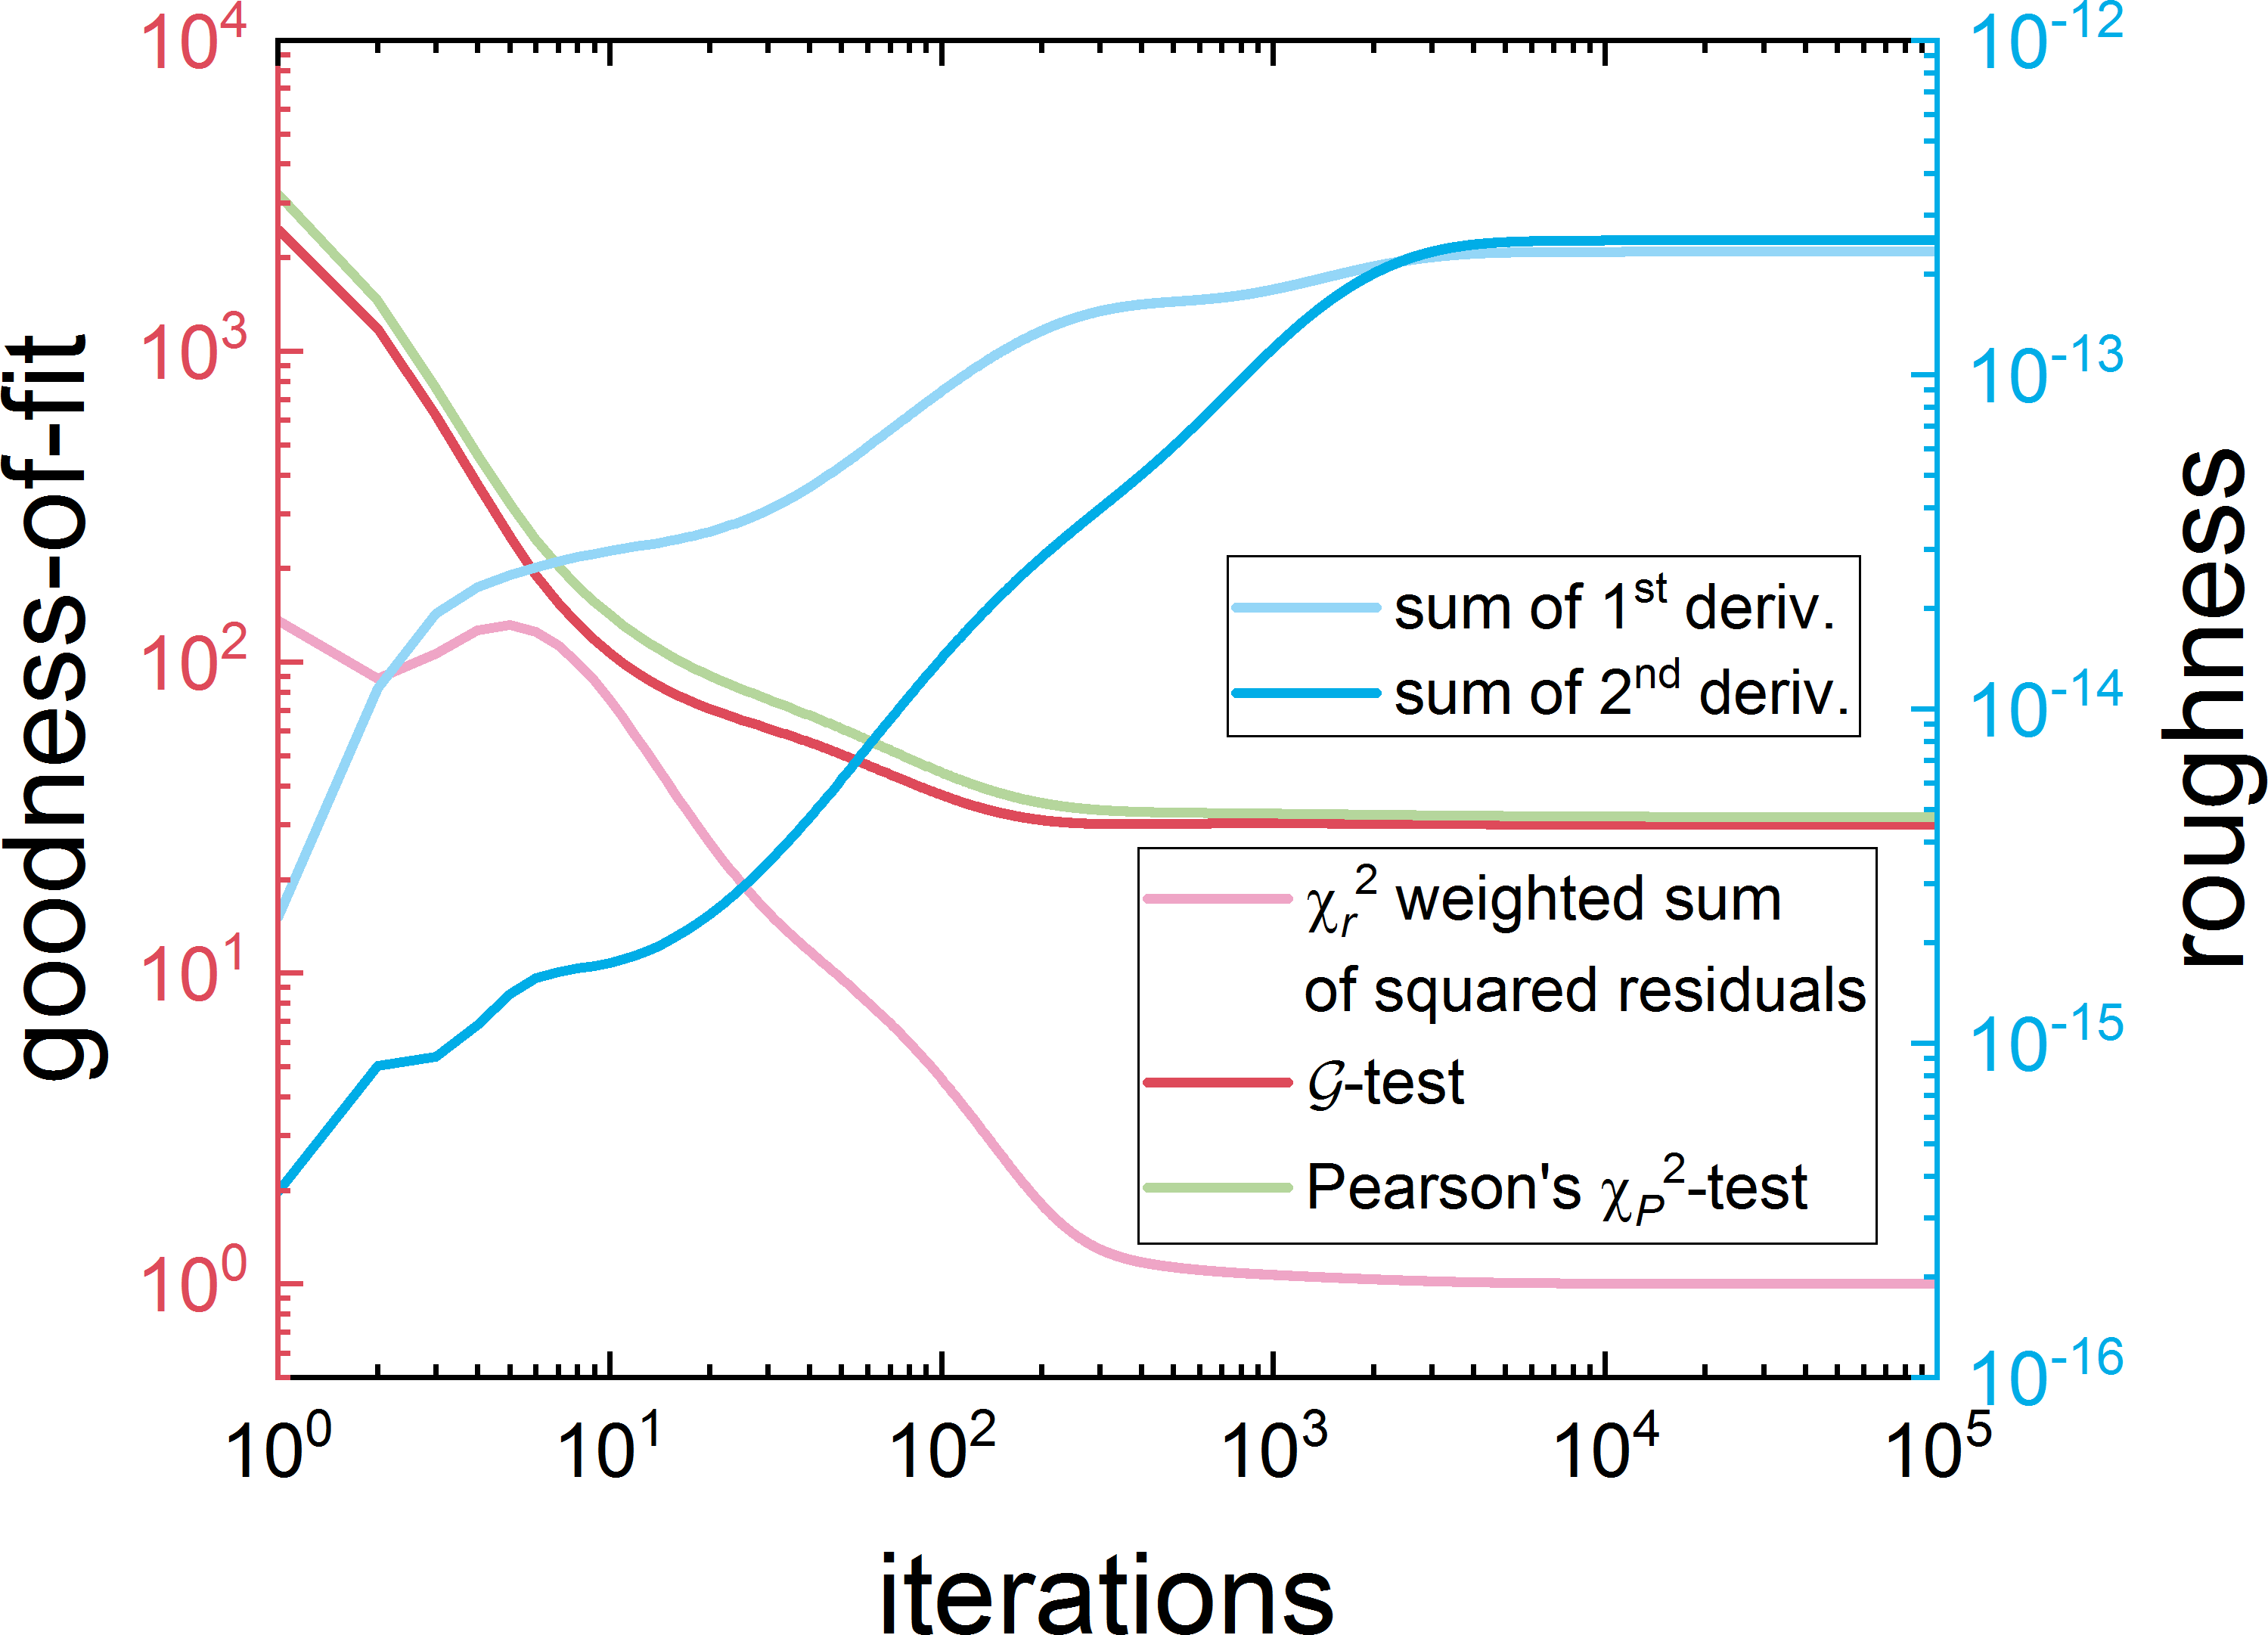
\includegraphics[width=0.48\textwidth]{../images/form_factor/EM/EMconstant_seed_smooth_0_000187_goodness_of_fit.png}
\hspace{0.06\textwidth}
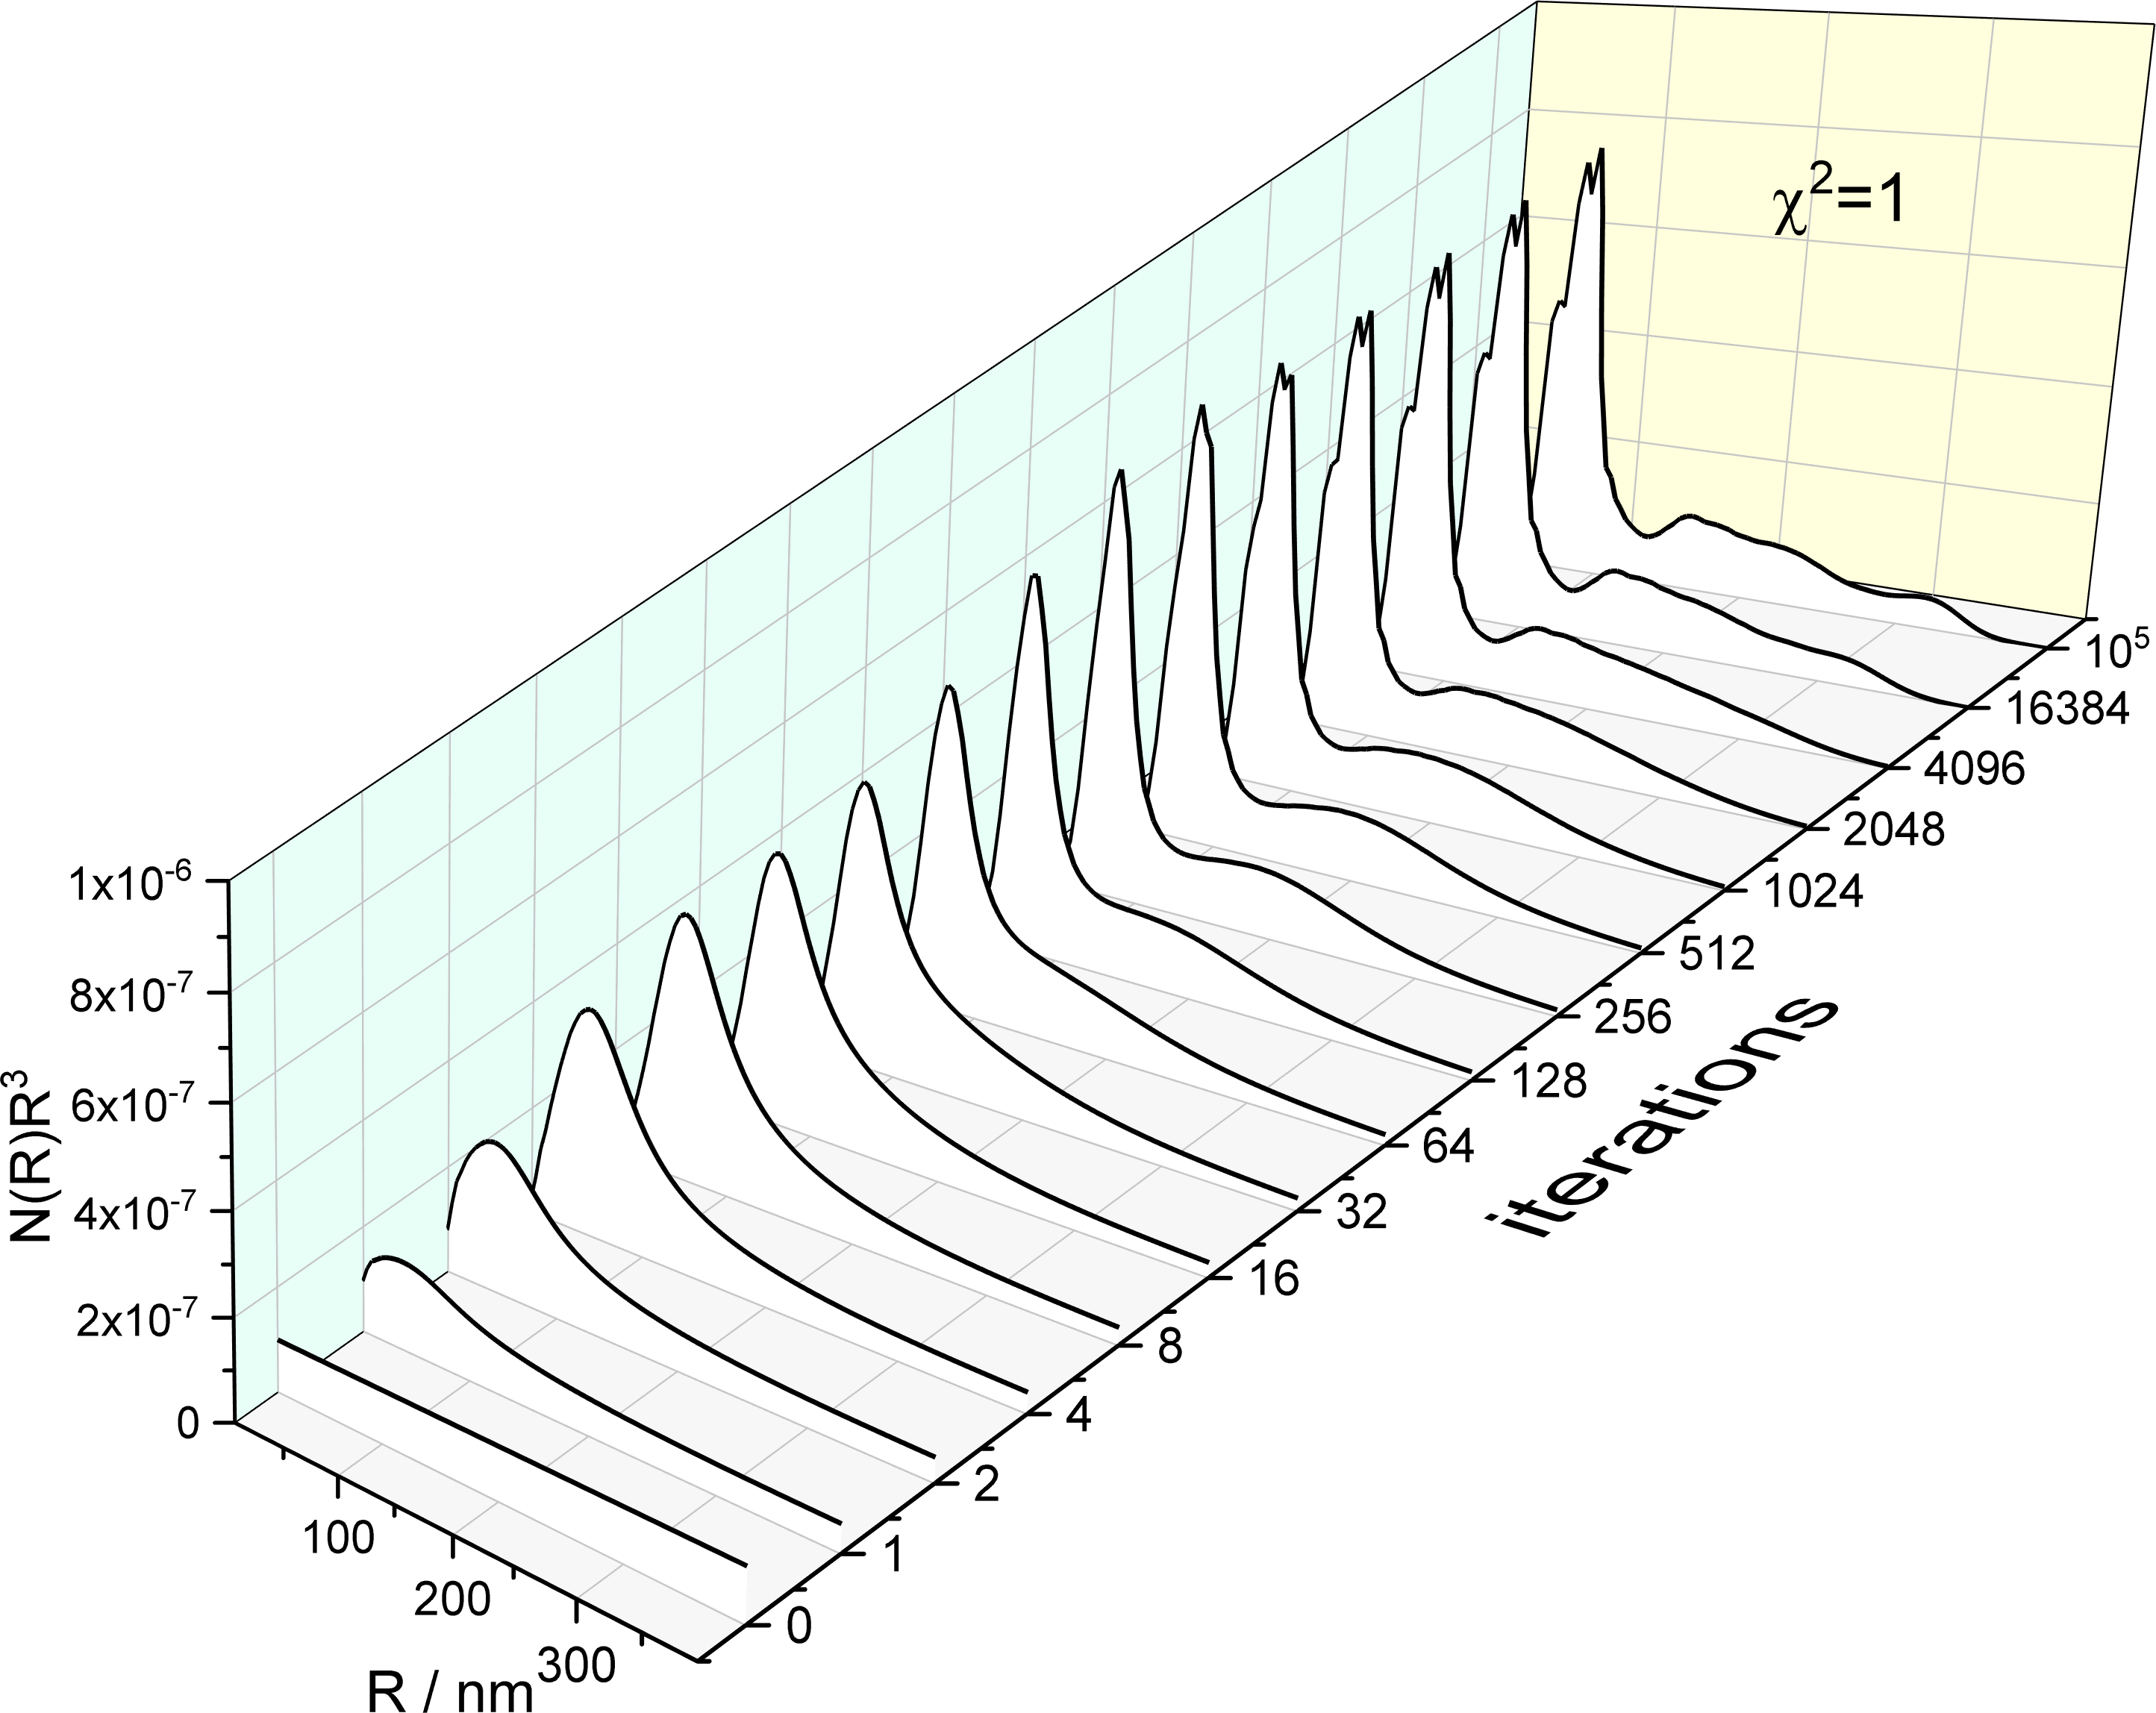
\includegraphics[width=0.42\textwidth]{../images/form_factor/EM/EMconstant_seed_smooth_0_000187_NR.png}
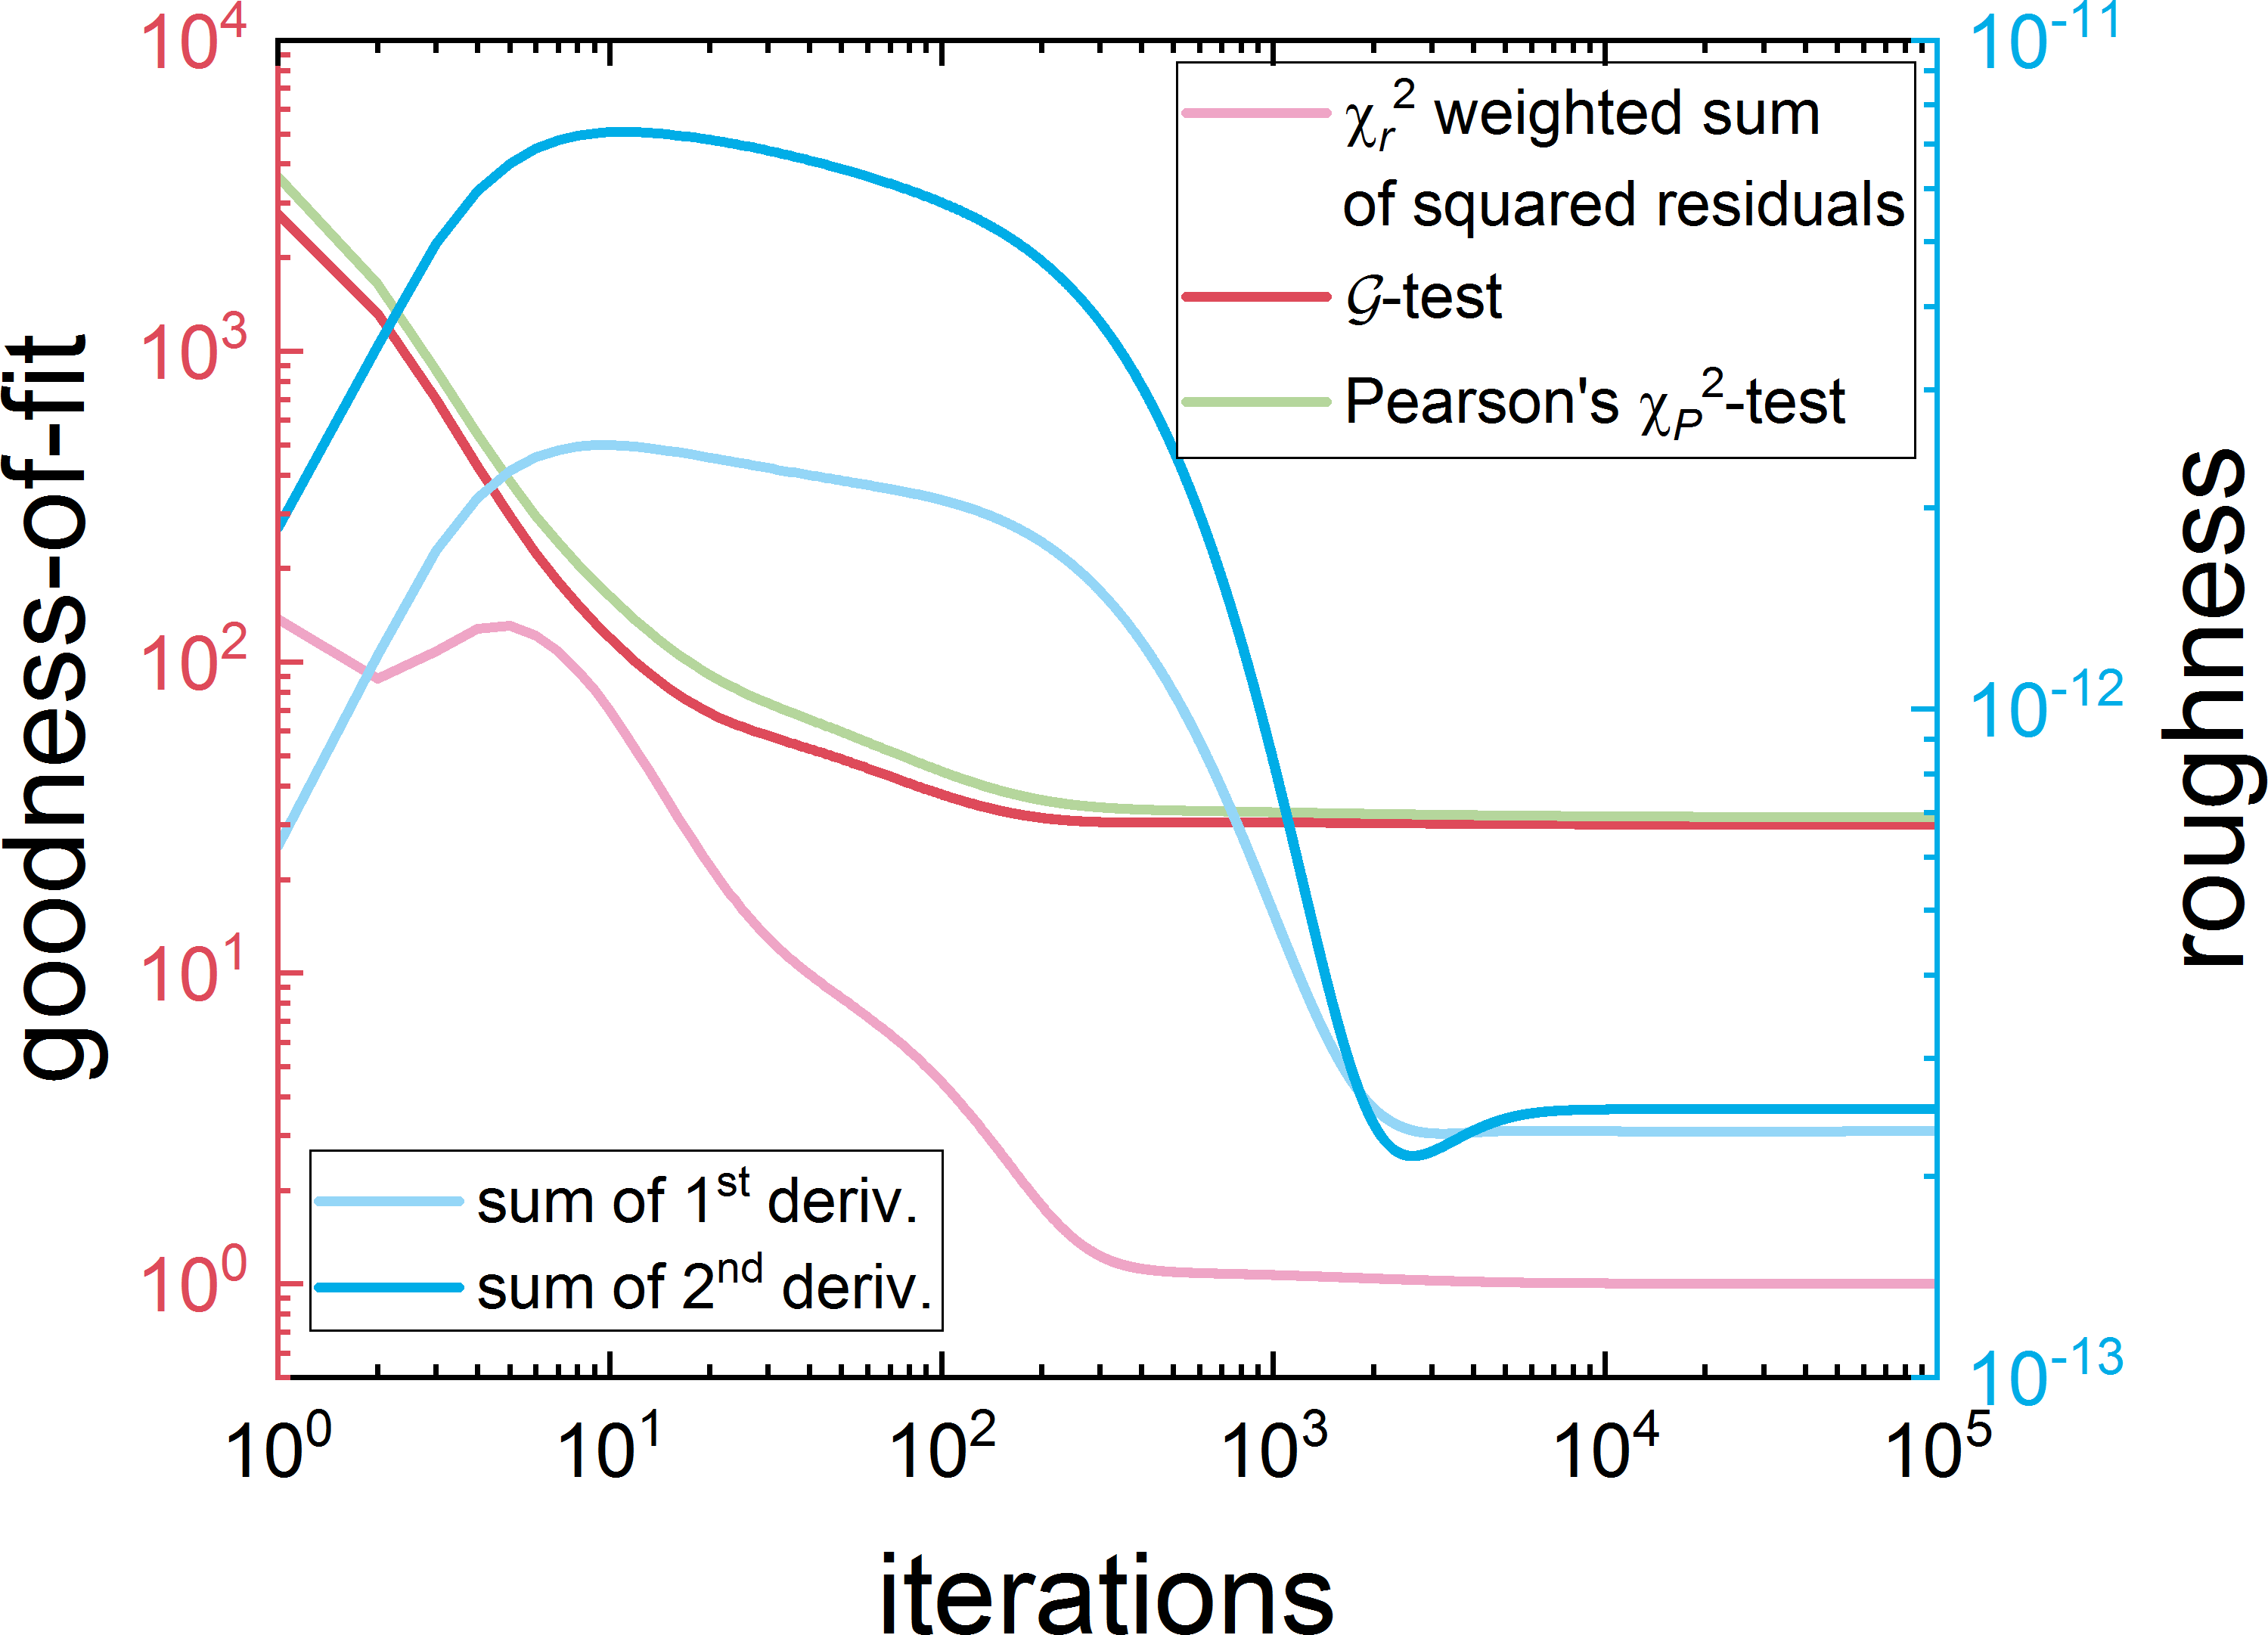
\includegraphics[width=0.48\textwidth]{../images/form_factor/EM/EMrandom_seed_smooth_0_000187_goodness_of_fit.png}
\hspace{0.06\textwidth}
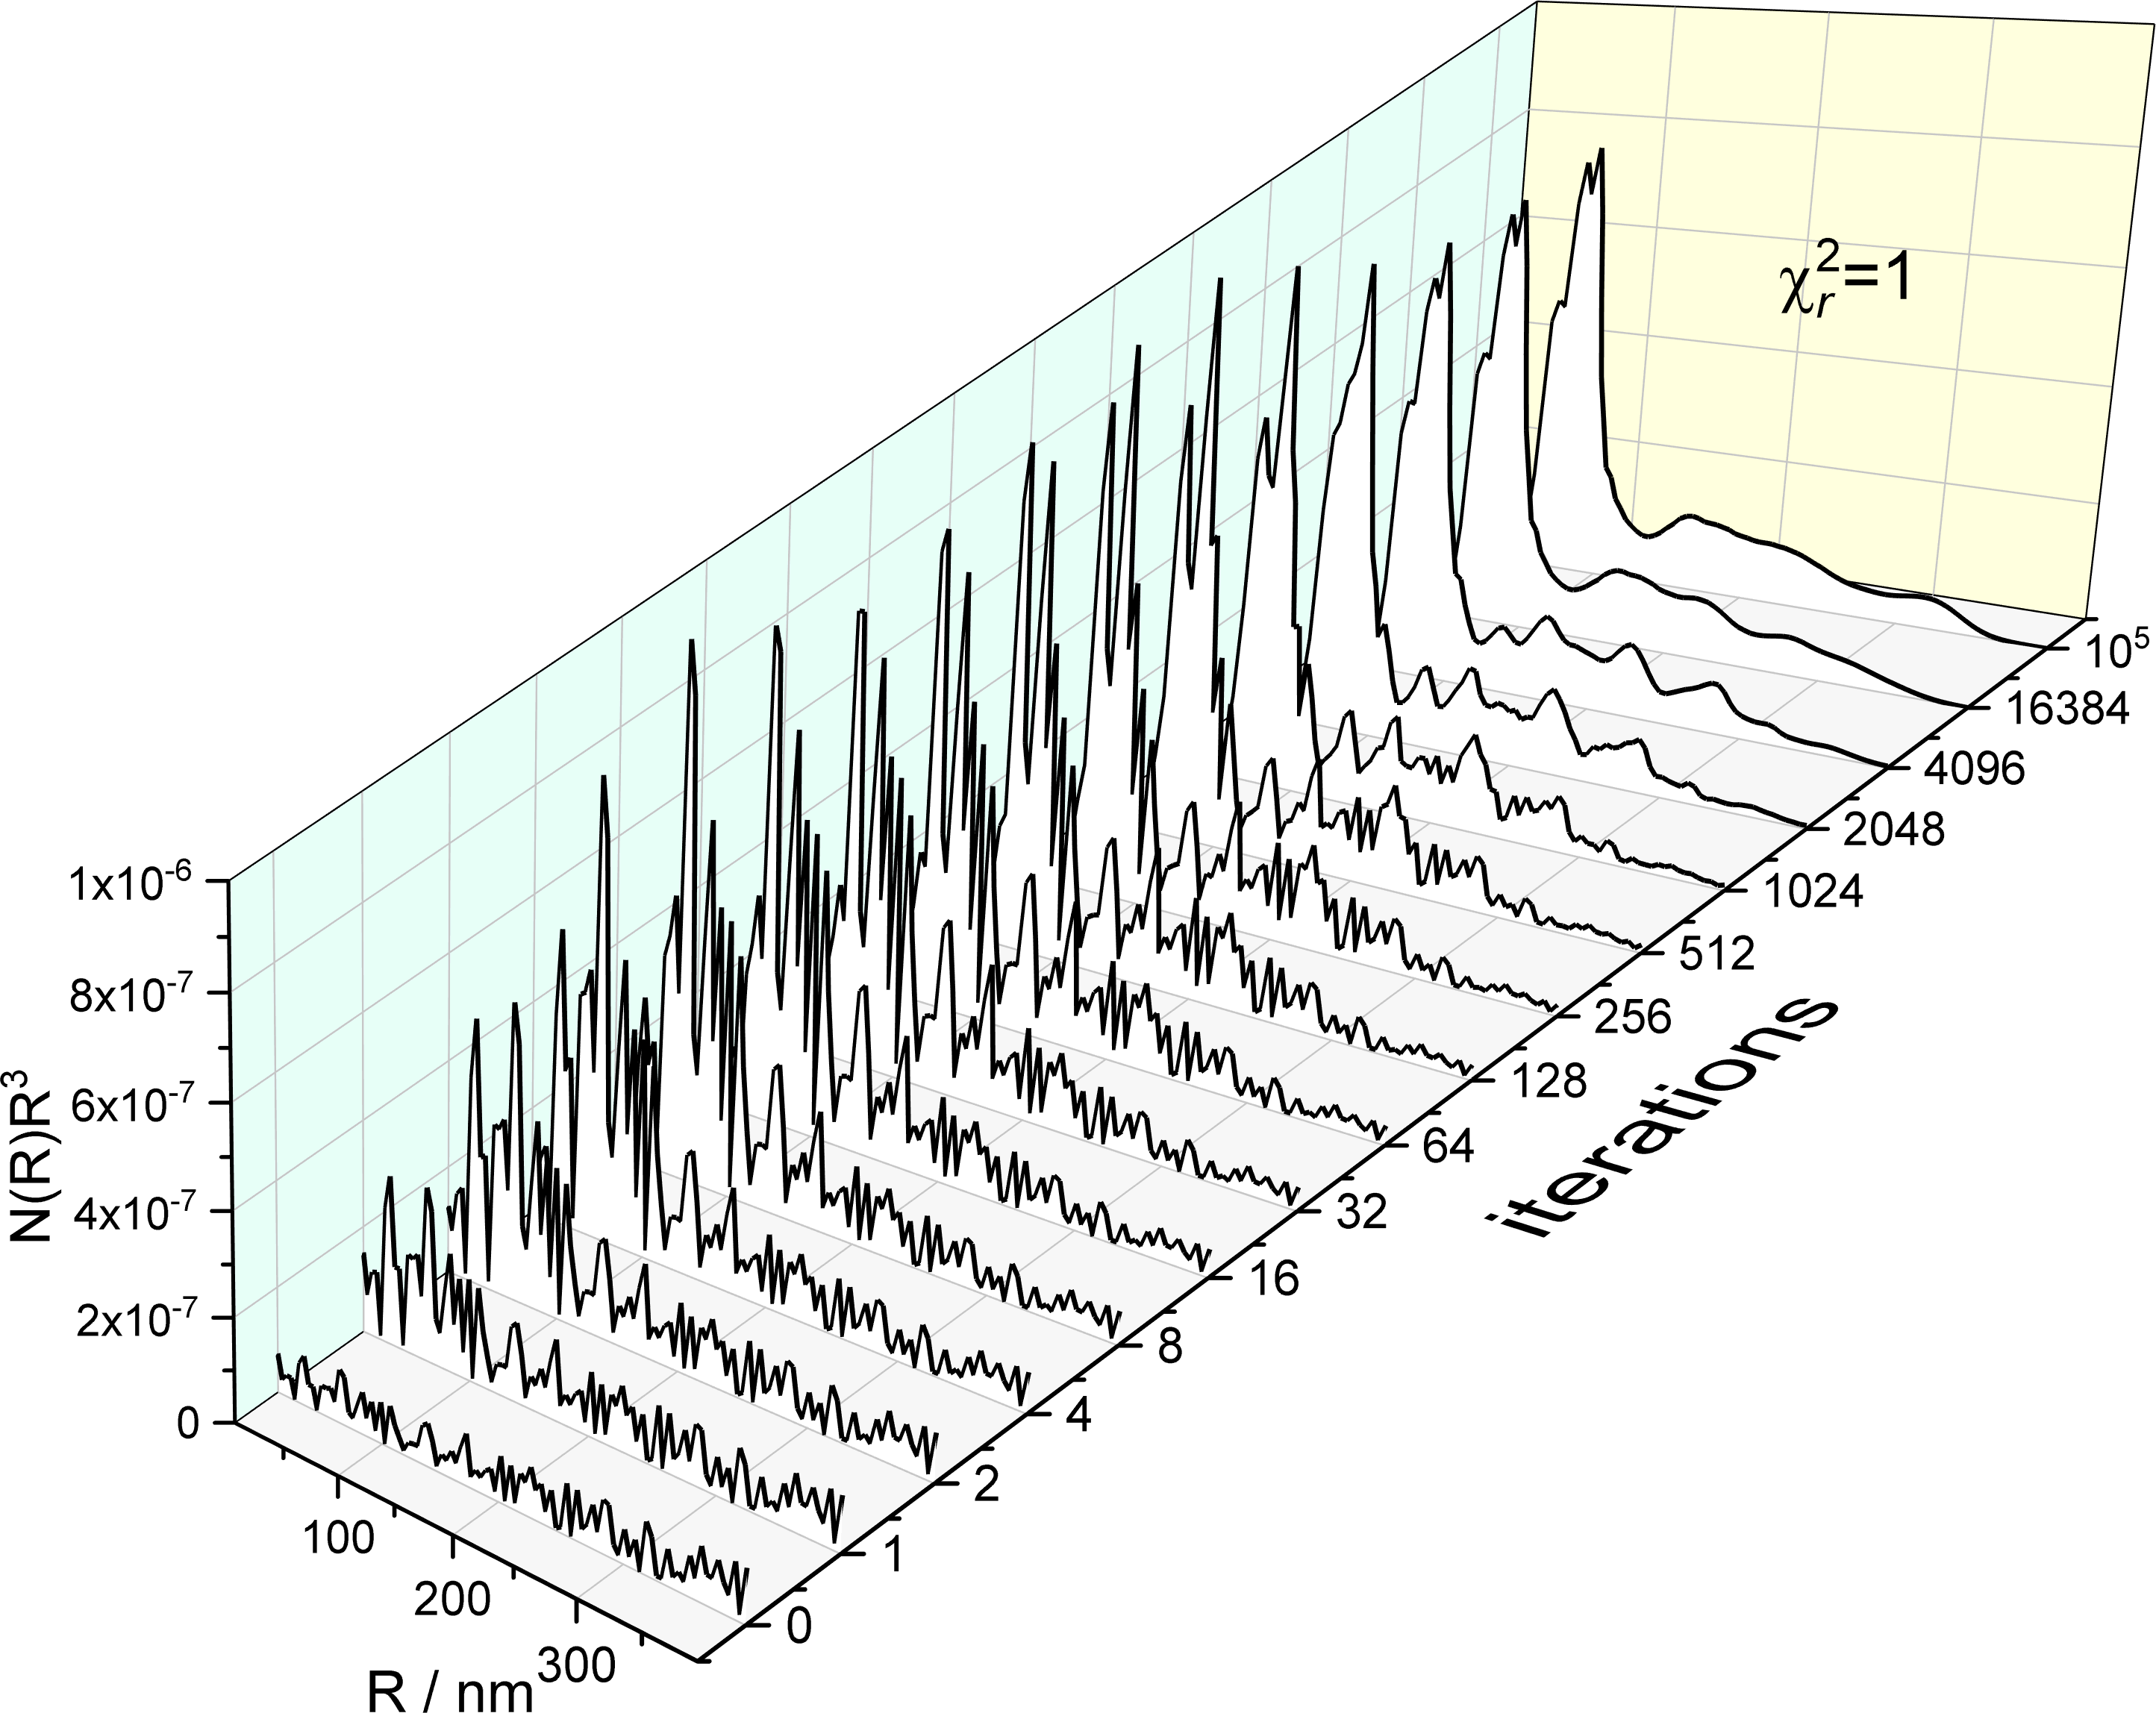
\includegraphics[width=0.42\textwidth]{../images/form_factor/EM/EMrandom_seed_smooth_0_000187_NR.png}
\caption{Roughness and goodness-of-fit parameters as well as the resulting volume distribution $N(R)R^3$ as a function of iterations for  a constant seed value (top) and random seed values (bottom) for an optimum soothing parameter $h=1.87\times 10^{-4}$ leading to $\chi_r^2=1$.\label{fig:EMhoptimum}}
\end{figure}

\begin{figure}[htb]
\centering
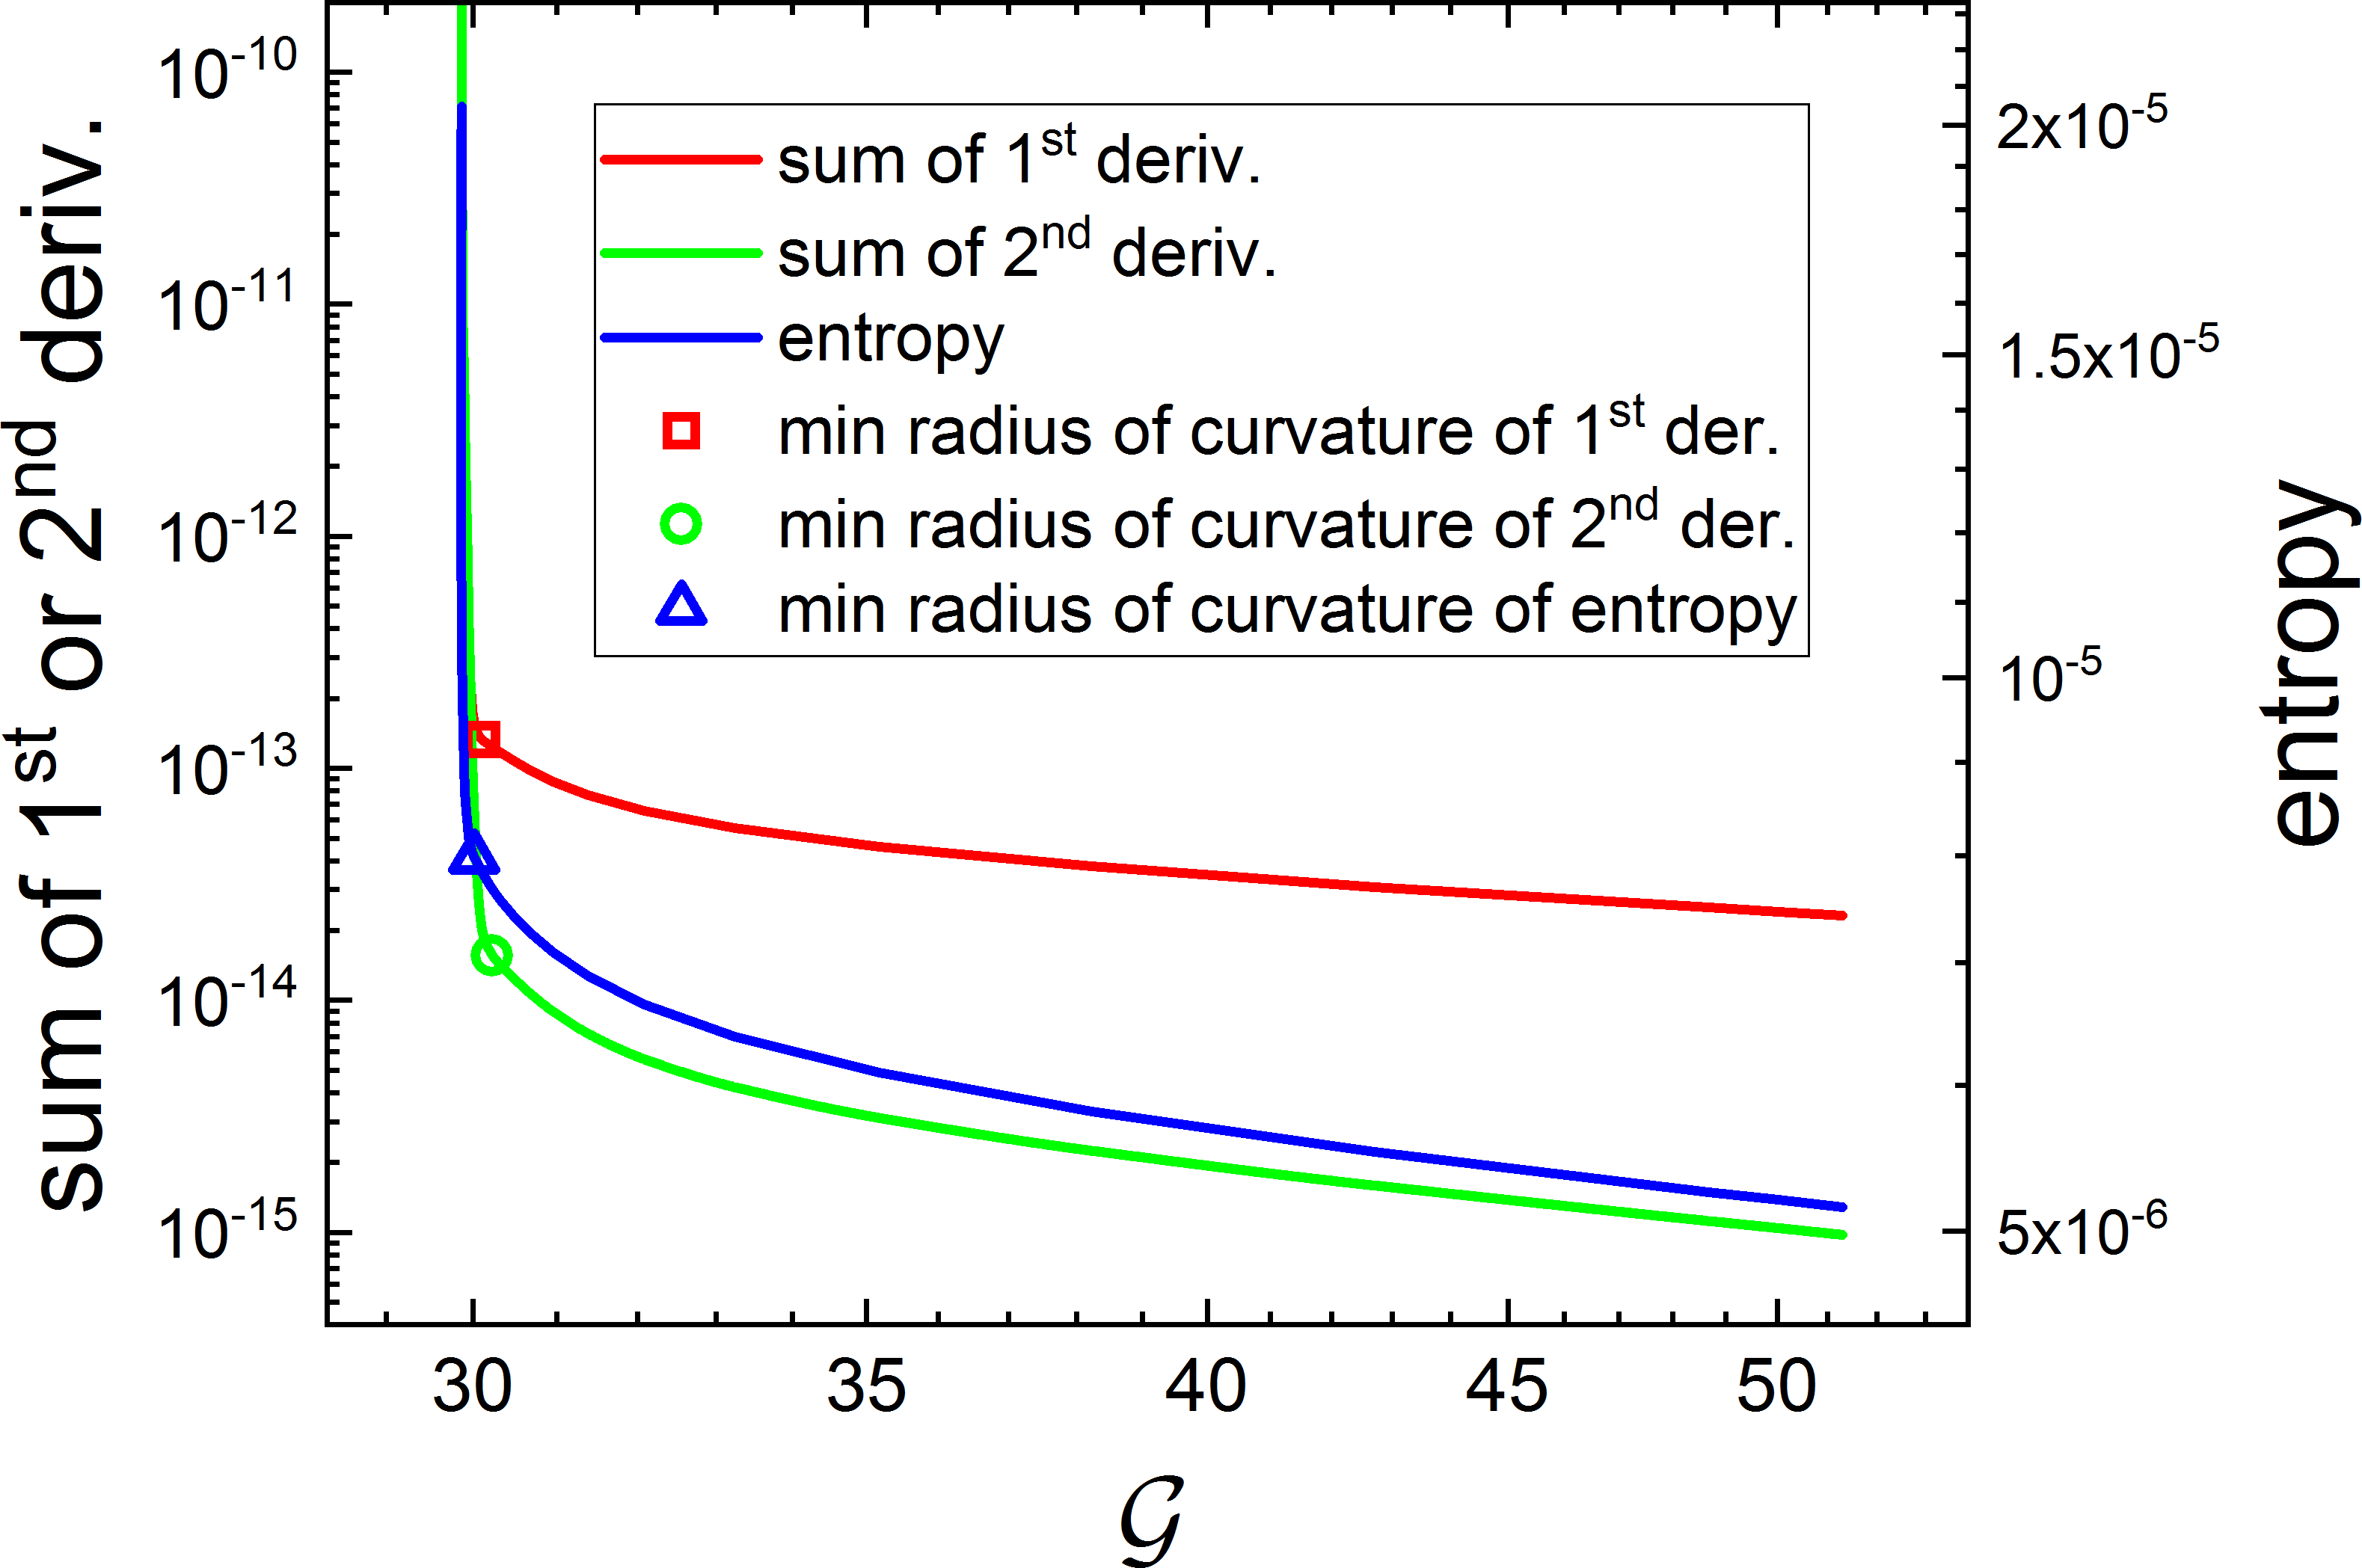
\includegraphics[width=0.65\textwidth]{../images/form_factor/EM/EMsmoothLcurves.png}
\caption{Optimum smoothing parameter $h$ given by the corner of the L-curve.\label{fig:EMhLcurve}}
\end{figure}

\begin{figure}[htb]
\centering
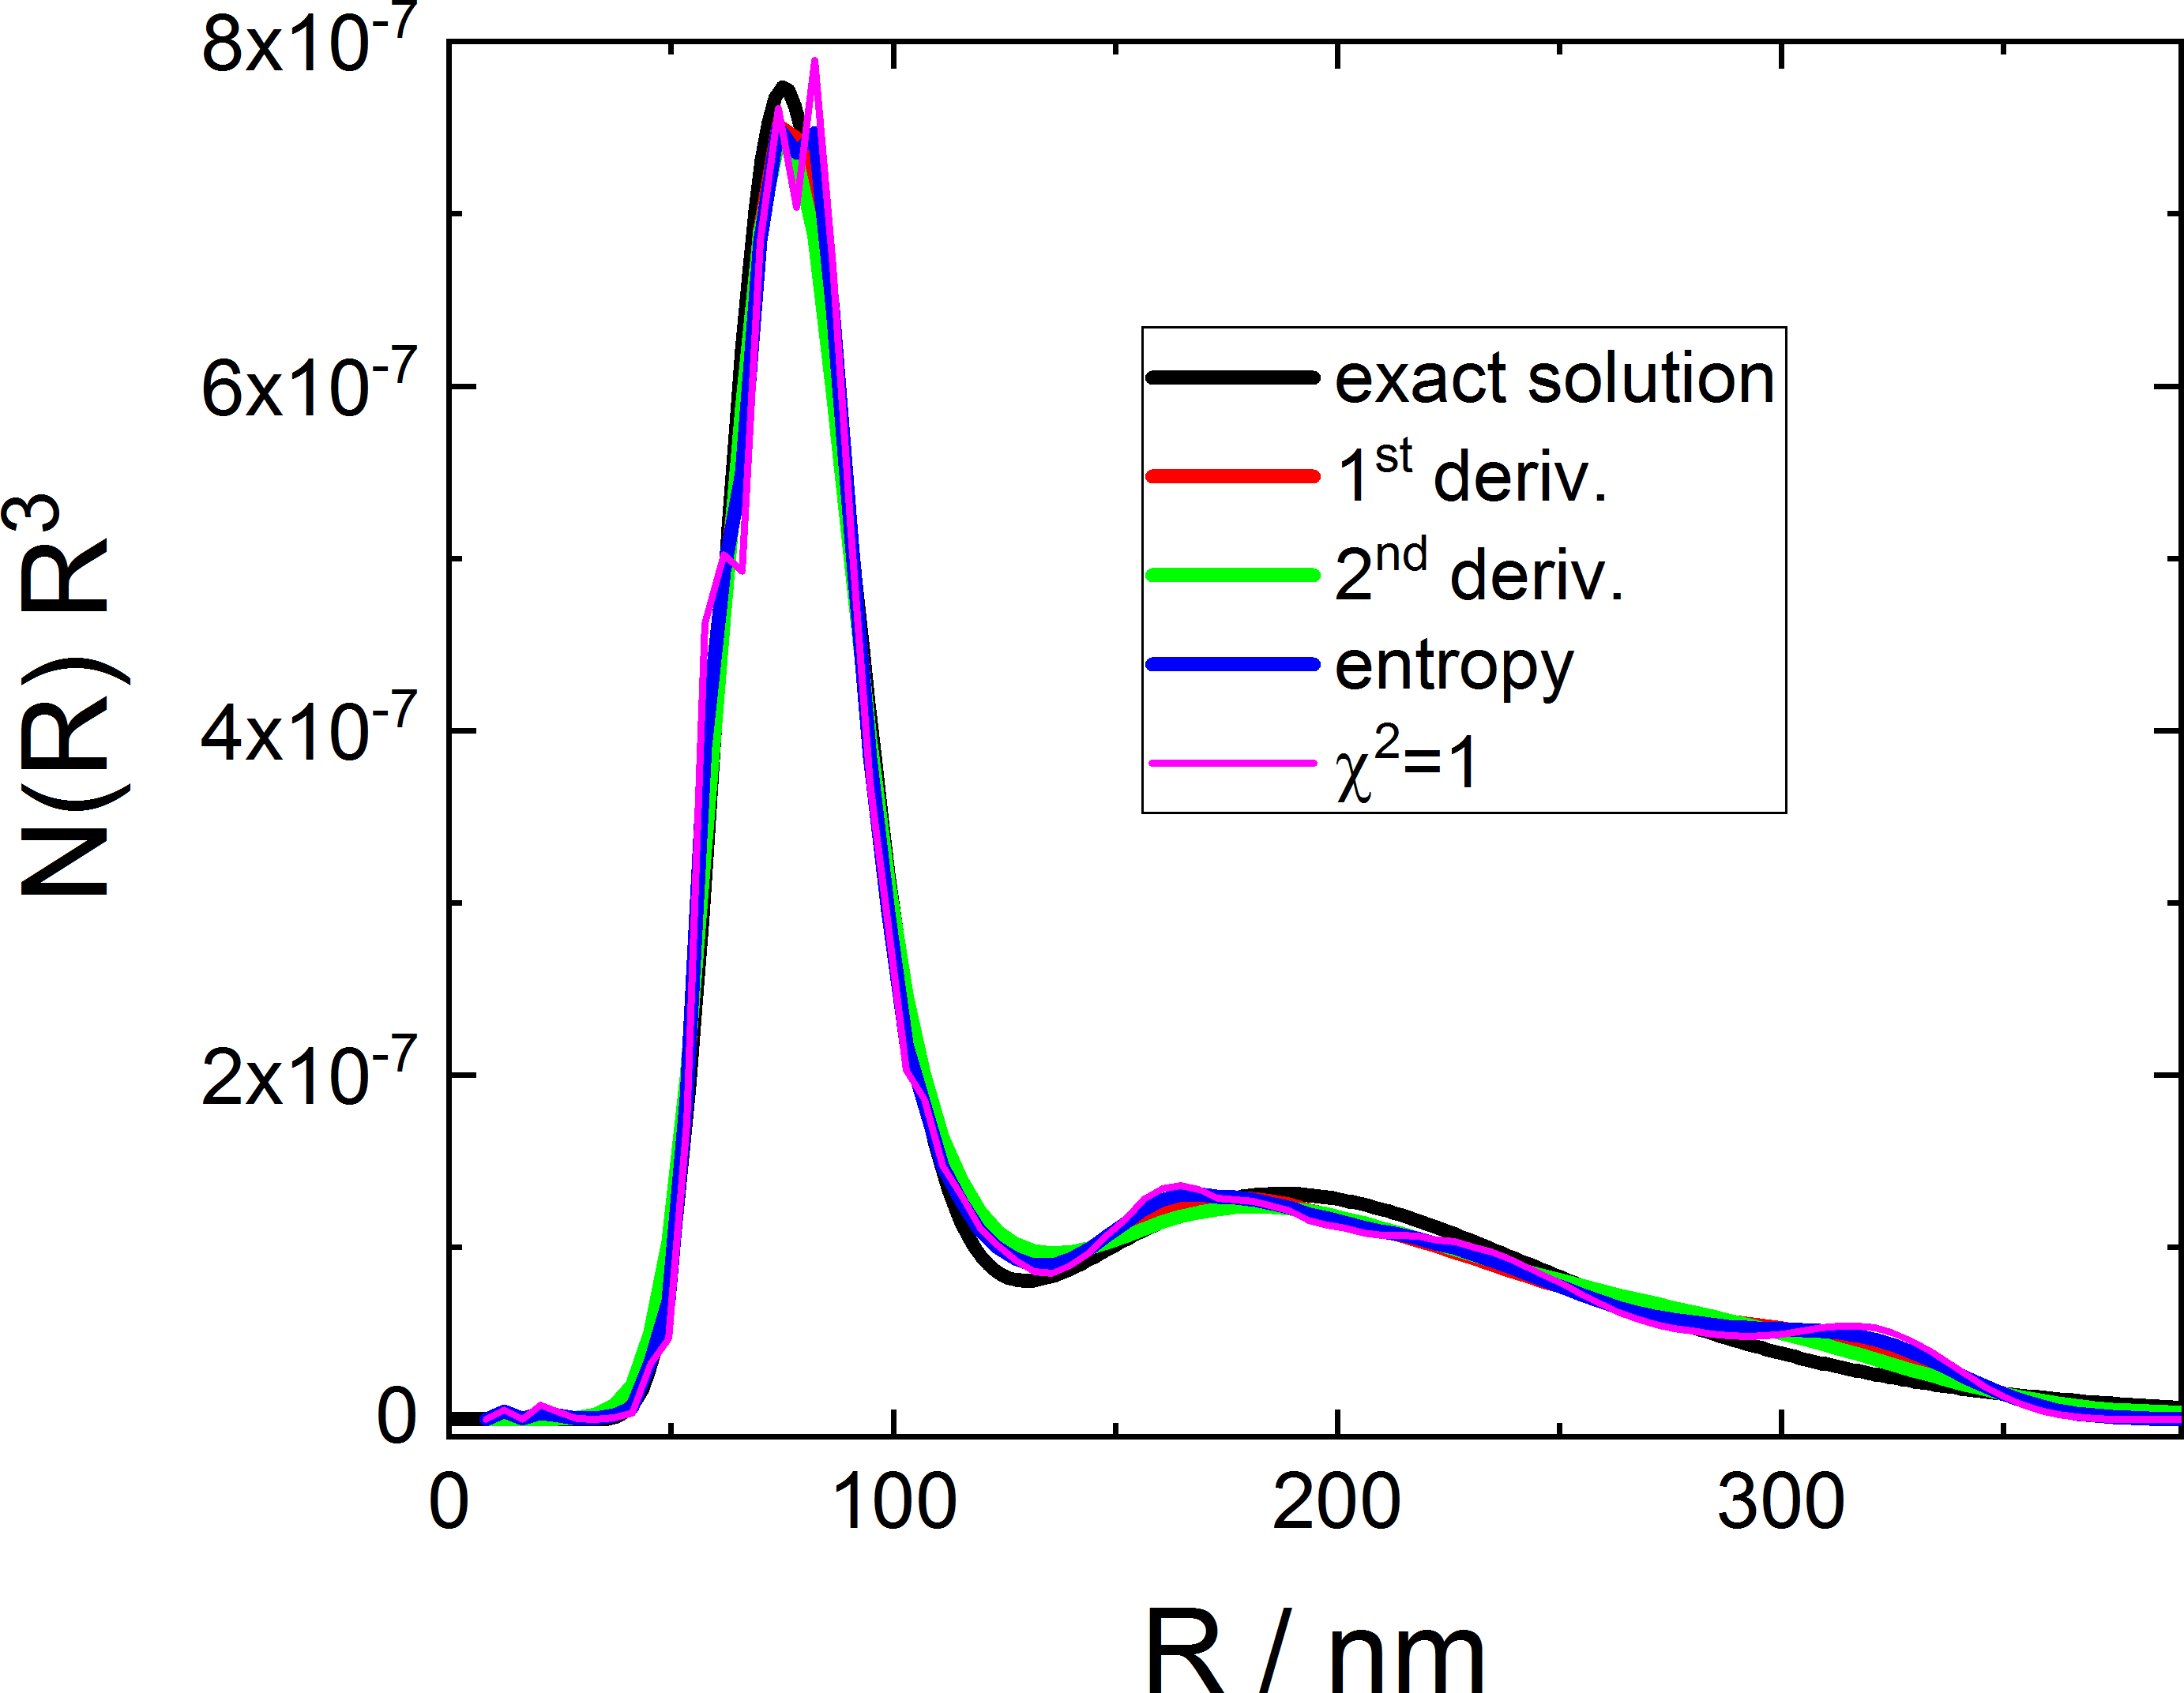
\includegraphics[width=0.6\textwidth]{../images/form_factor/EM/EMsmoothNRR3.png}
\caption{The smoothing parameters has been obtained by the corners of the L-curves in fig.\ \ref{fig:EMhLcurve} and the solution of the EM iteration scheme with double smoothing is compared with the exact solution.\label{fig:EMsmoothNRR3}}
\end{figure}

The proper choice of the parameter $h$ arises and its selection might follow similar strategies than for the regularization parameter in ill-posed problems. In contrast to regularization methods in this iteration scheme there is not directly a penalty term (a measure for the smoothness/roughness of the solution) involved like the sum of first or second derivatives of the solution vector or the entropy of the solution vector like in maximum entropy methods. However, these quantity can easily be calculated from the solution vector. Figure \ref{fig:EMLcurves} shows the logarithm of a roughness term, namely the sum of 1$^\mathrm{st}$ and 2$^\mathrm{nd}$ derivatives of the resulting size distribution and the entropy against the goodness-of-fit parameter from eq.\ \ref{eq:goodnessoffit_Gtest}, namely the ``$\mathcal{G}$-test'' parameter. The optimum smoothing parameter has been defined via the corner of the L-curve defined by $(\log(\mathcal{G}),\log(|| \hat{\mathbf{L}} \mathbf{x} ||^2))$, with $\hat{\mathbf{L}}$ being the first or second-order discrete derivative operator defined in eq.\ \ref{eq:first_derivative_penalty} or \ref{eq:second_derivative_penalty} and by $(\log(\mathcal{G}),\log(S))$ with $S$ being the entropy defined in eq.\ \ref{eq:EMentropy}. The corners were determined numerically as they are defined by having the maximum curvature. They are marked in fig.\ \ref{fig:EMhLcurve} by a symbols. The whole analysis does not make use of the uncertainties of the measured intensities. If the error bars are trustable and the model for the form factor is correct the weighted sum of squared residuals should be $\chi_r^2= 1$. This can also be used as a condition for determining the smoothing parameter $h$. In the case of the present analysed data both strategies yield similar results as can be seen in fig.\ \ref{fig:EMsmoothNRR3}.

~\\

\subsection{EM with maximum entropy regularization}~\\
The Lucy\hyp{}Richardson method \cite{Richardson1972,Lucy1974} has been extended by an additional penalty function,
namely the entropy, by Lucy \cite{Lucy1994}. He introduces two variants, how the maximum entropy penalty can be introduced in the iteration algorithm by knowing either a fixed or assuming an adaptive prior for the solution vector. The entropy $S$ is given by
\begin{align}
S&= \sum_{j=0}^{N-1} -x_j\ln\left(x_j/m_j\right) +x_j-m_j \label{eq:EMentropy}
\end{align}
with $\mathbf{m}$ being the prior estimate of $\mathbf{x}$. The update scheme in eq.\ \ref{eq:LucyRichardsonInversionMethod} has to be extended as
\begin{align}
\label{eq:LucyRichardsonInversionMethodMEconstant}
  x_j^{(k+1)} &= x_j^{(k)} + \Delta x_j^{(k)} + \Delta s_j^{(k)}= \mathcal{O}_\mathrm{EM,ME,const}\left[x_j^{(k)}\right]
\end{align}
with
\begin{align}
  \Delta x_j^{(k)} &= x_j^{(k)}\left[\sum_{i=0}^{M-1}\frac{A_{ij}}{\left(\displaystyle \sum_{m=0}^{M-1}A_{mj}\right)}\frac{b_i}{\displaystyle \sum_{n=0}^{N-1}A_{in}x_n^{(k)}}-1\right] \\
  \Delta s_j^{(k)} &=  \lambda x_j^{(k)}\left(-\ln\frac{x_j}{m_j}+\frac{1}{\sum_{j=0}^{N-1}x_j^{(k)}}\sum_{j=0}^{N-1}x_j^{(k)}\ln\frac{x_j^{(k)}}{m_j}\right)
\end{align}
in case of a known prior. If a prior is not known a constant prior can be chosen. However, even if no model for the prior is known, one can try to construct one adaptively according to Horne \cite{Horne1985} by applying for example a Gaussian point spread function to the actual solution and using this as a prior for the next iteration step. In this case the update scheme looks as
\begin{align}
\label{eq:LucyRichardsonInversionMethodMEadaptive}
  x_j^{(k+1)} &= x_j^{(k)} + \Delta x_j^{(k)} + \Delta s_j^{(k)}= \mathcal{O}_\mathrm{EM,ME,adaptive}\left[x_j^{(k)}\right]\\
  \Delta x_j^{(k)} &= x_j^{(k)}\left[\sum_{i=0}^{M-1}\frac{A_{ij}}{\left( \sum_{m=0}^{M-1}A_{mj}\right)}\frac{b_i}{ \sum_{n=0}^{N-1}A_{in}x_n^{(k)}}-1\right] \\
  \Delta s_j^{(k)} &=  \lambda x_j^{(k)}\left(-\ln\frac{x_j}{m_j^{(k)}}
                                +\frac{1}{\sum_{j=0}^{N-1}x_j^{(k)}}\sum_{j=0}^{N-1}x_j^{(k)}\ln\frac{x_j^{(k)}}{m_j^{(k)}}
                                -1+\sum_{i=0}^{N-1}\Pi_{ij}\frac{x_i^{(k)}}{m_i^{(k)}}\right) \\
  m_i^{(k)} &= \sum_{j=0}^{N-1}\Pi_{ij}x_j^{(k)}
\end{align}
As a smoothing operator for the prior
\begin{align}\label{eq:smoothingOp4prior}
  \Pi_{ij} &= \frac{1}{c}\exp\left(-\frac{(i-j)^2}{2\sigma^2}\right)
\end{align}
has been assumed with the normalization constant $c=\sum_j \Pi_{ij}$ and a $\sigma^2$ typically between $\frac12$ and 2. For large values of $\sigma^2$ the results converge to that one of a constant prior. For too small values the regularization is suppressed as the prior converges to the $k^\mathrm{th}$ iteration step.

The optimum regularization parameter $\lambda$ can be determined similar to the previous section via the corner in the L-curve. The L-curves for both a constant and adaptive prior are shown in fig.\ \ref{fig:EMlambdaLcurve} using the same data than shown in fig.\ \ref{fig:EMIQevolution}. The optimum Lagrange parameter in the corner are marked with a symbol. The corresponding size distribution are shown in fig.\ \ref{fig:EMconstadaptiveNRR3} together wit the exact solution and for a Lagrange parameter leading to $\chi_r^2=1$. From the L-curves in fig.\ \ref{fig:EMlambdaLcurve} one can see, that the $\mathcal{G}$-test parameter for the constant prior varies over orders of magnitudes whereas for the adaptive prior also for a Lagrange parameter far away from its optimum value leads to a reasonable good result. Therefore the L-curve shows for the adaptive prior a much smaller range on the $x$-axis.

\begin{figure}[htb]
\centering
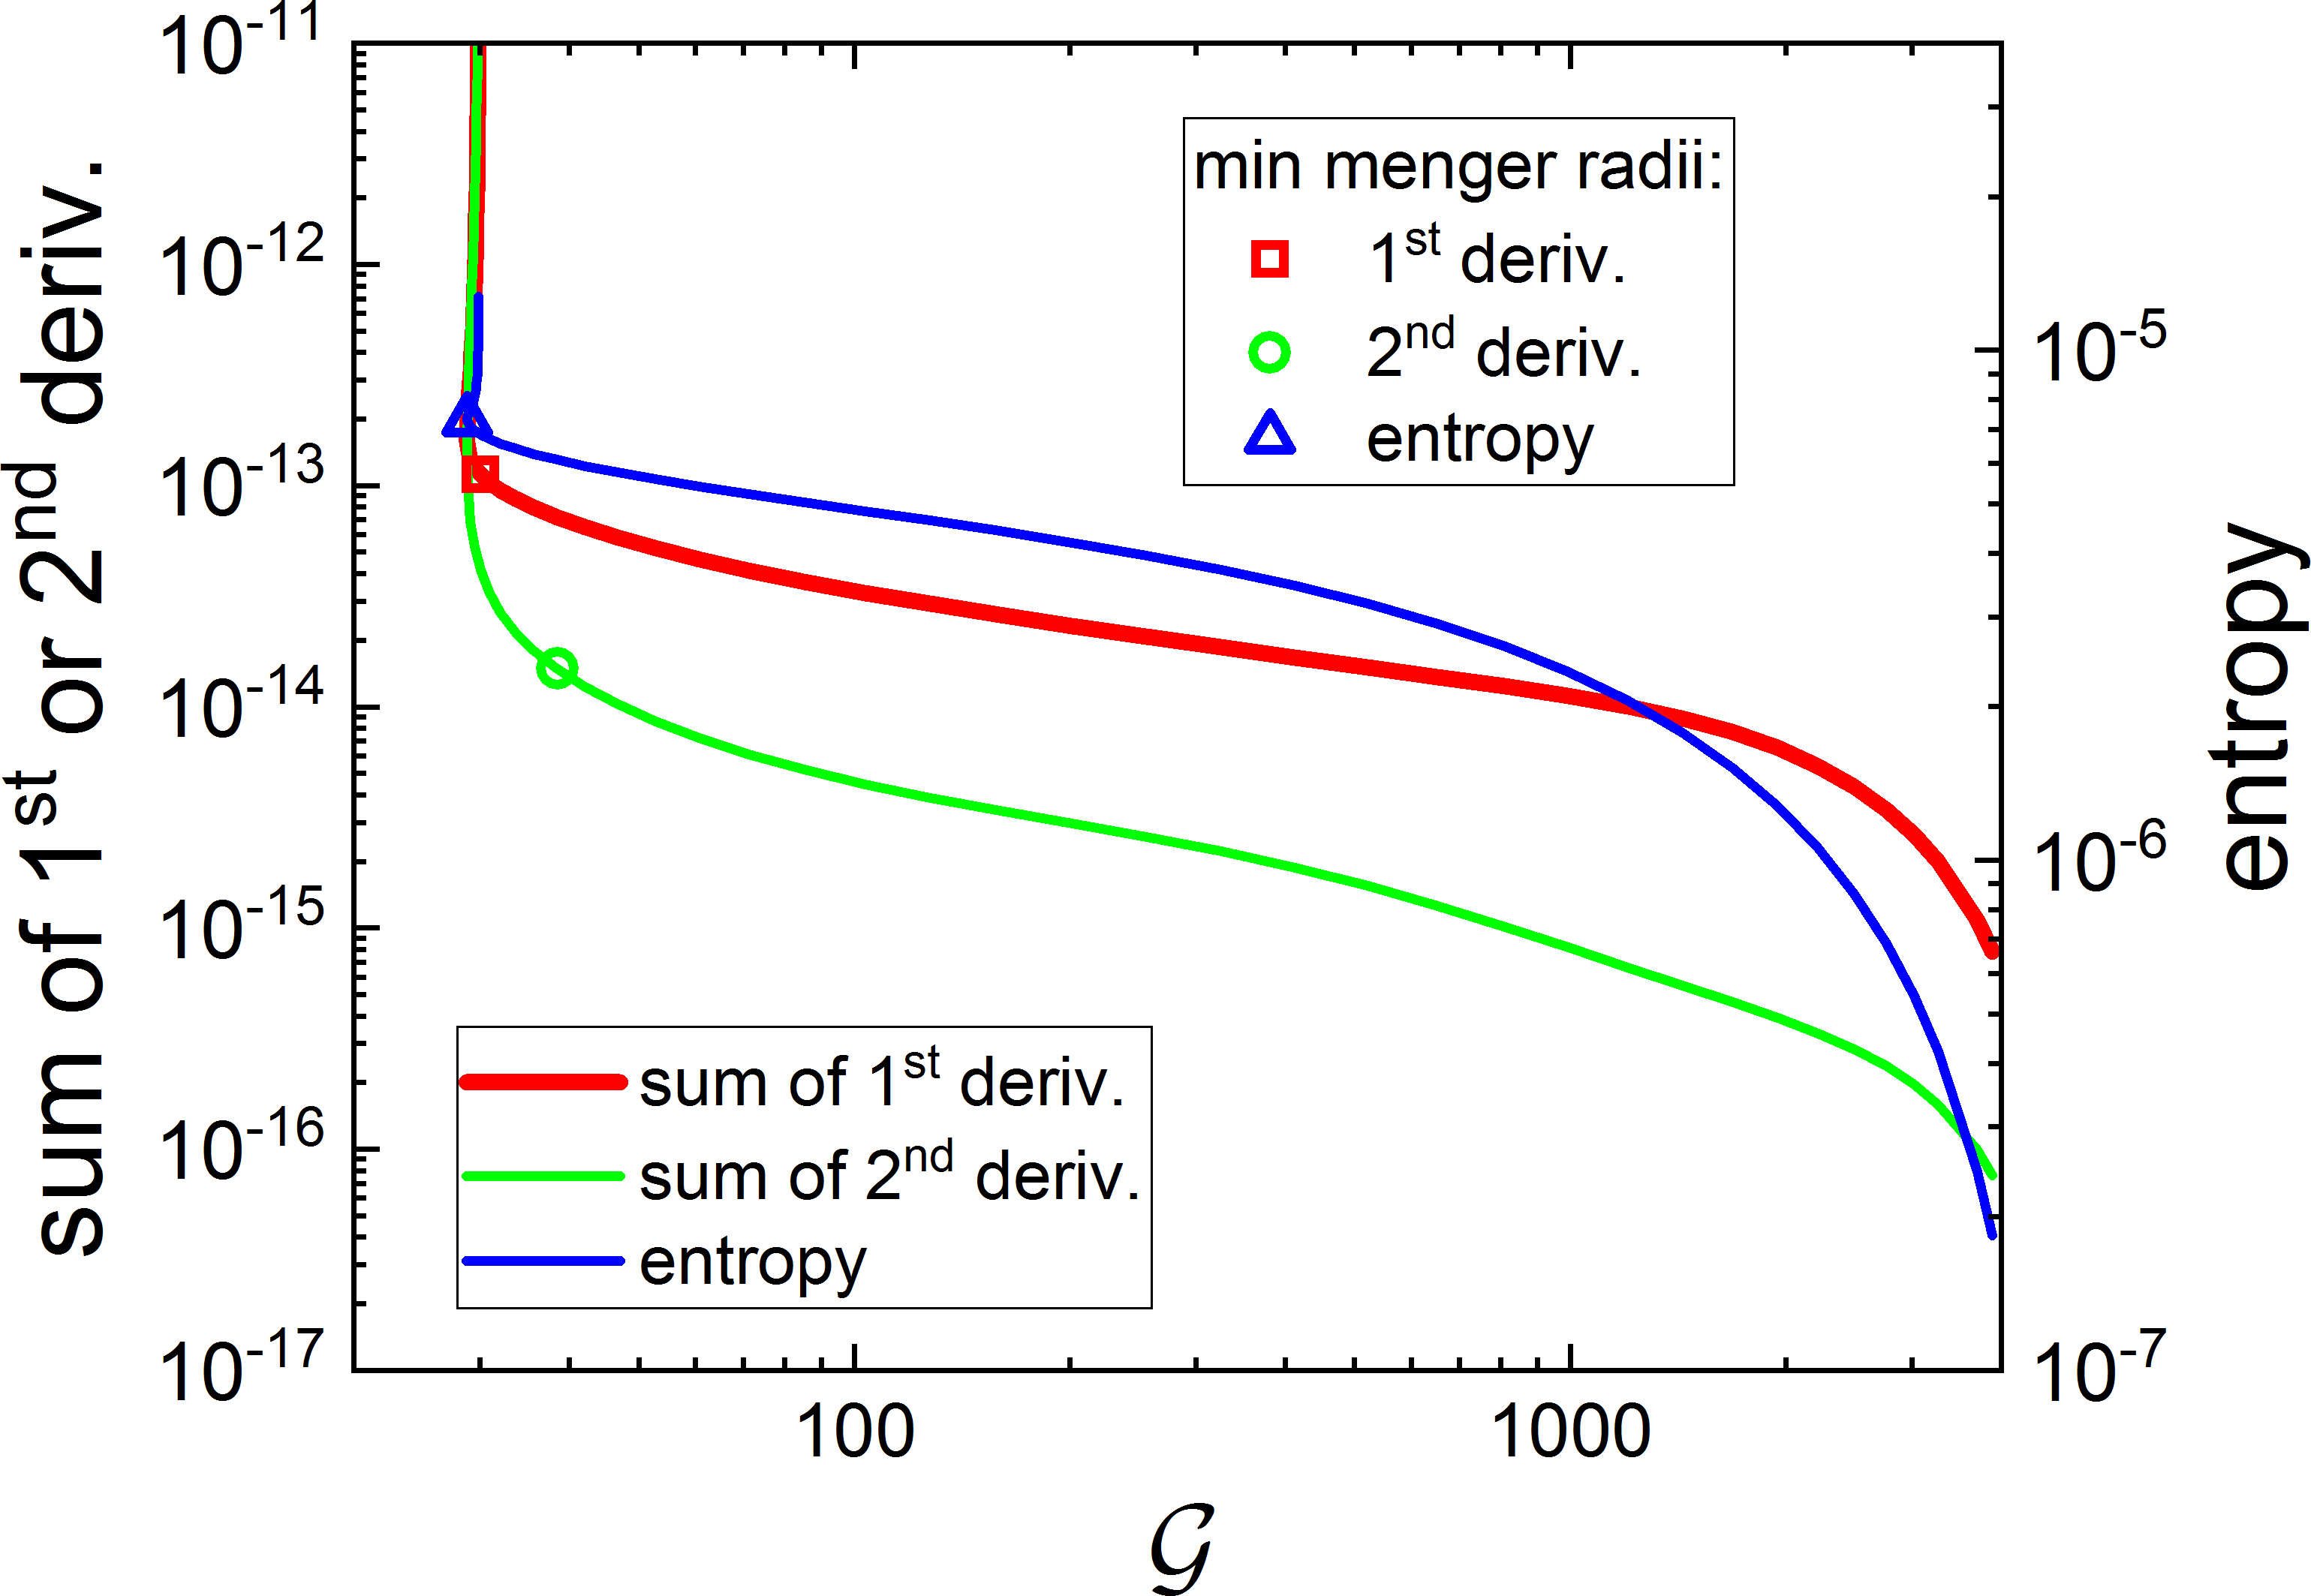
\includegraphics[width=0.42\textwidth]{../images/form_factor/EM/EMconstLcurve.png} \hspace{0.06\textwidth}
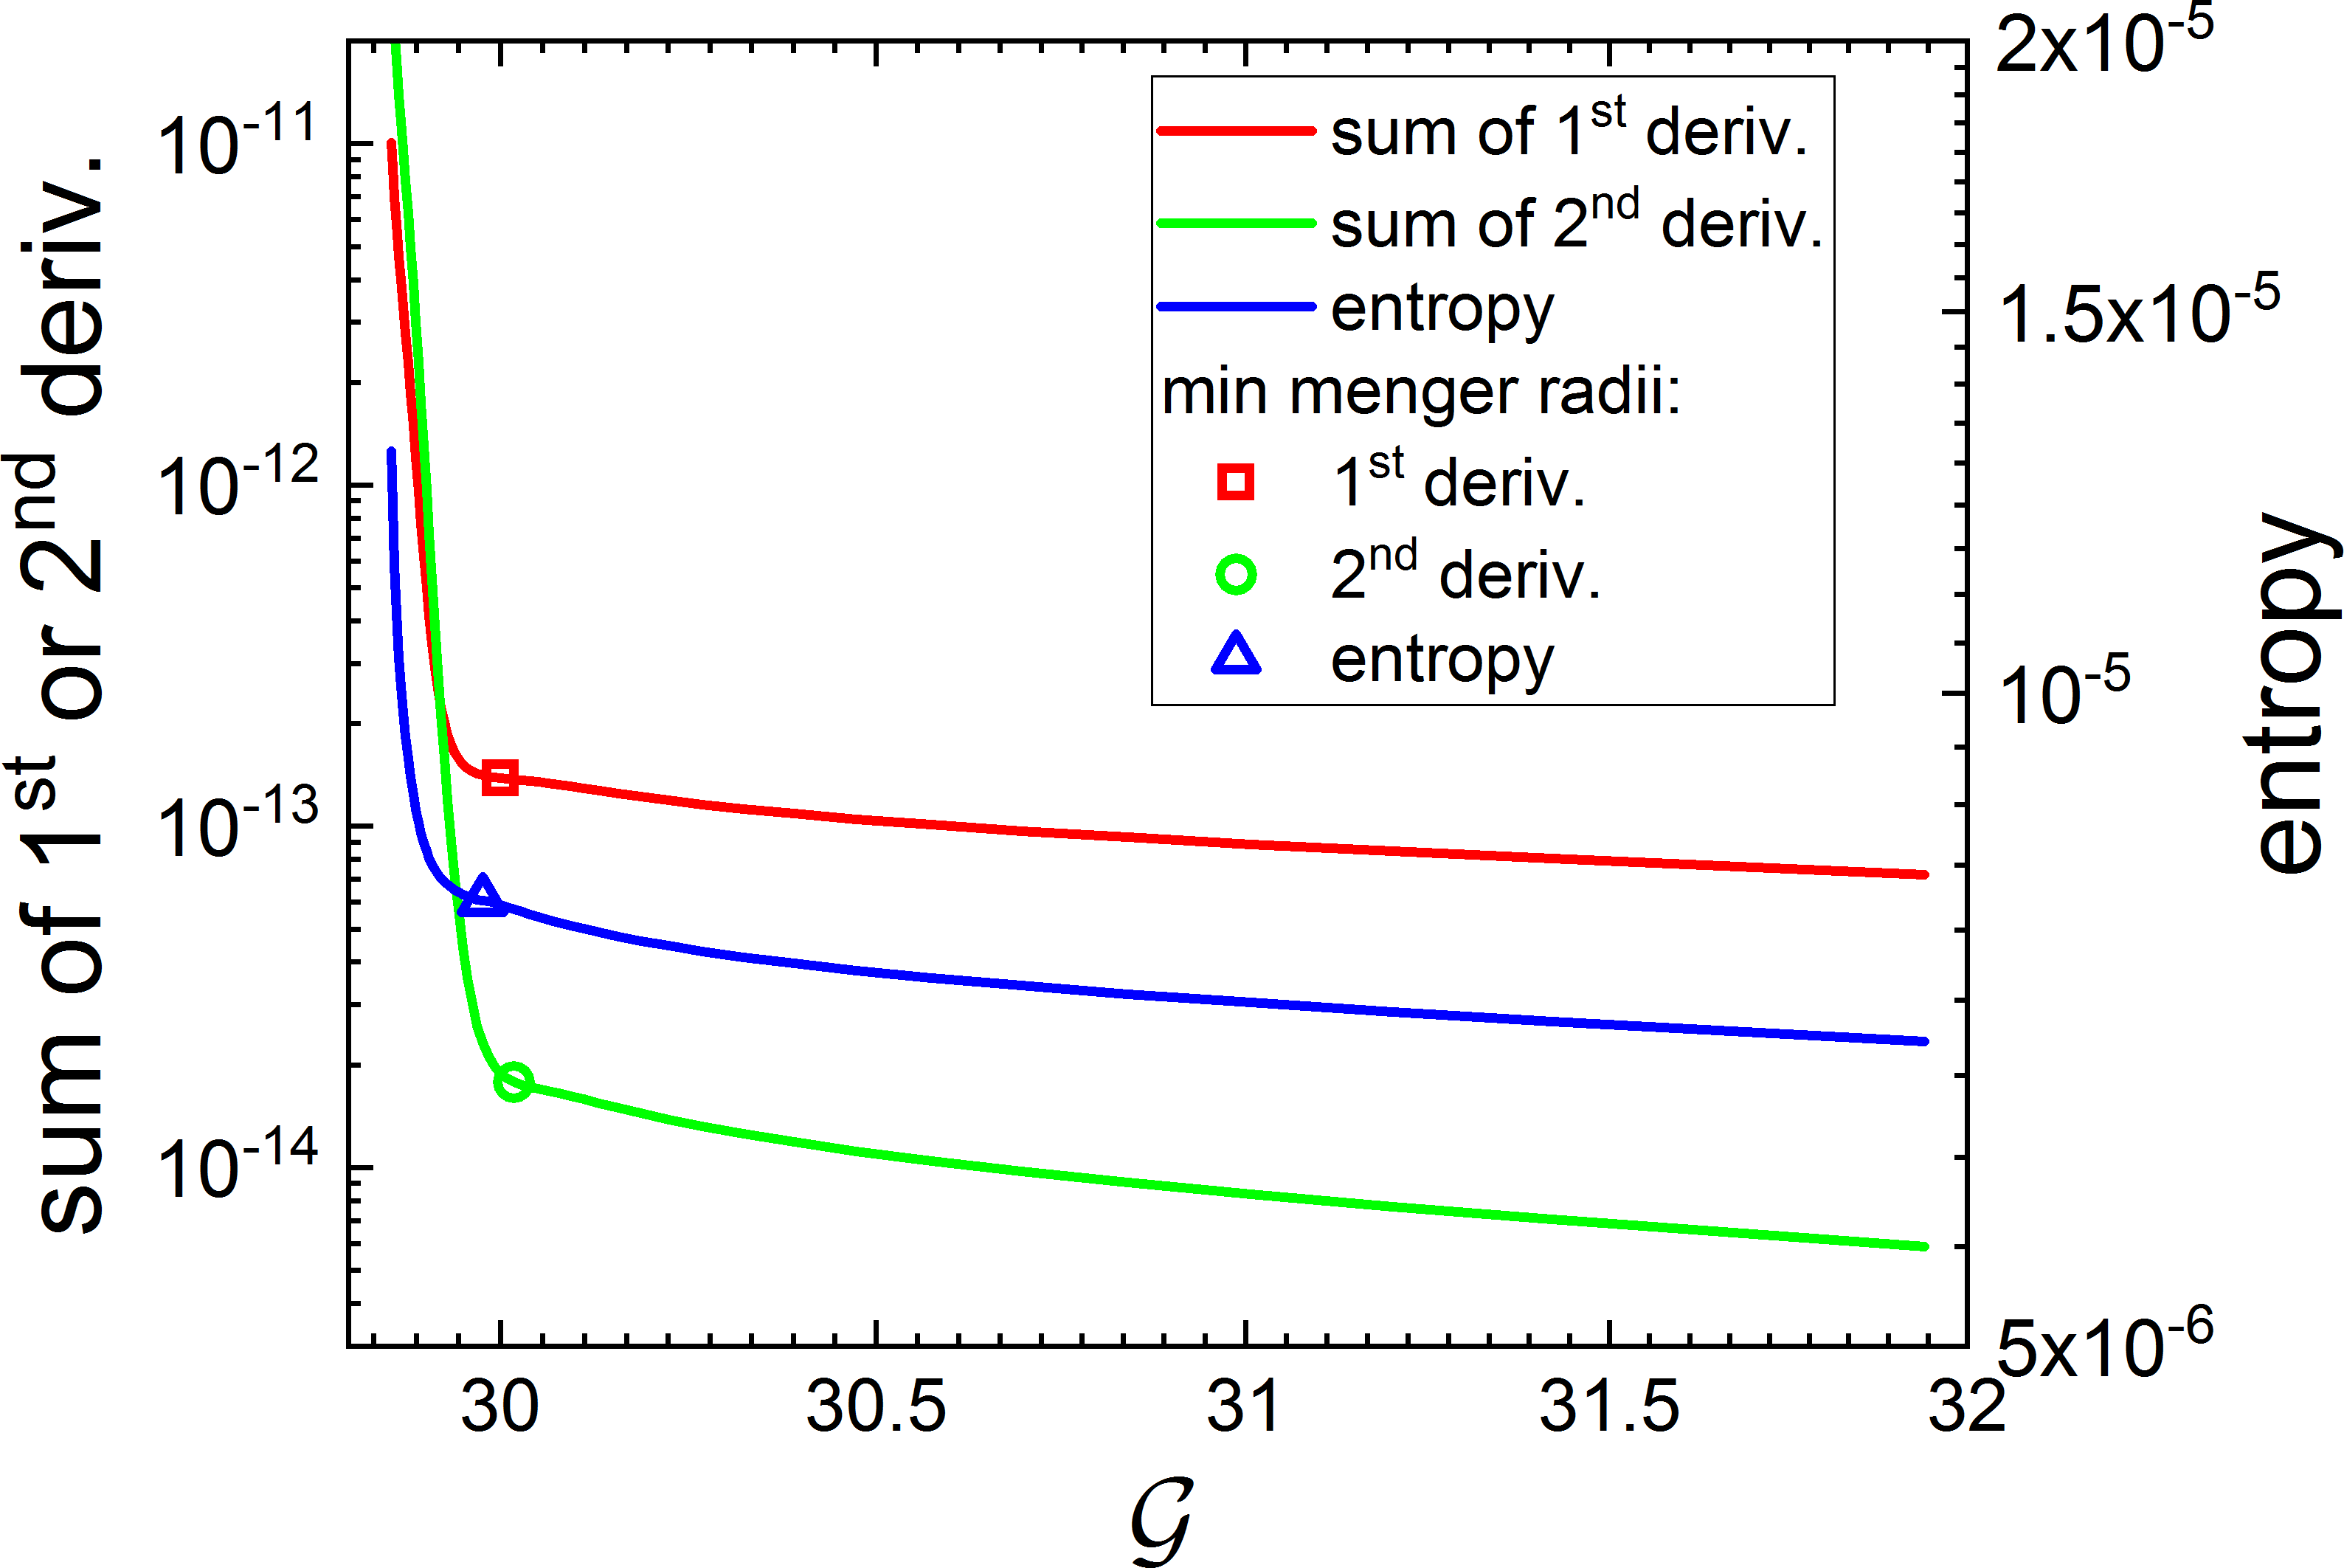
\includegraphics[width=0.42\textwidth]{../images/form_factor/EM/EMadaptiveLcurve.png}
\caption{Determine optimum smoothing parameter $\lambda$ by the corner of the L-curve, which is determined by a minimum radius of curvature. (left) constant prior, (right) adaptive prior\label{fig:EMlambdaLcurve}}
\end{figure}

\begin{figure}[htb]
\centering
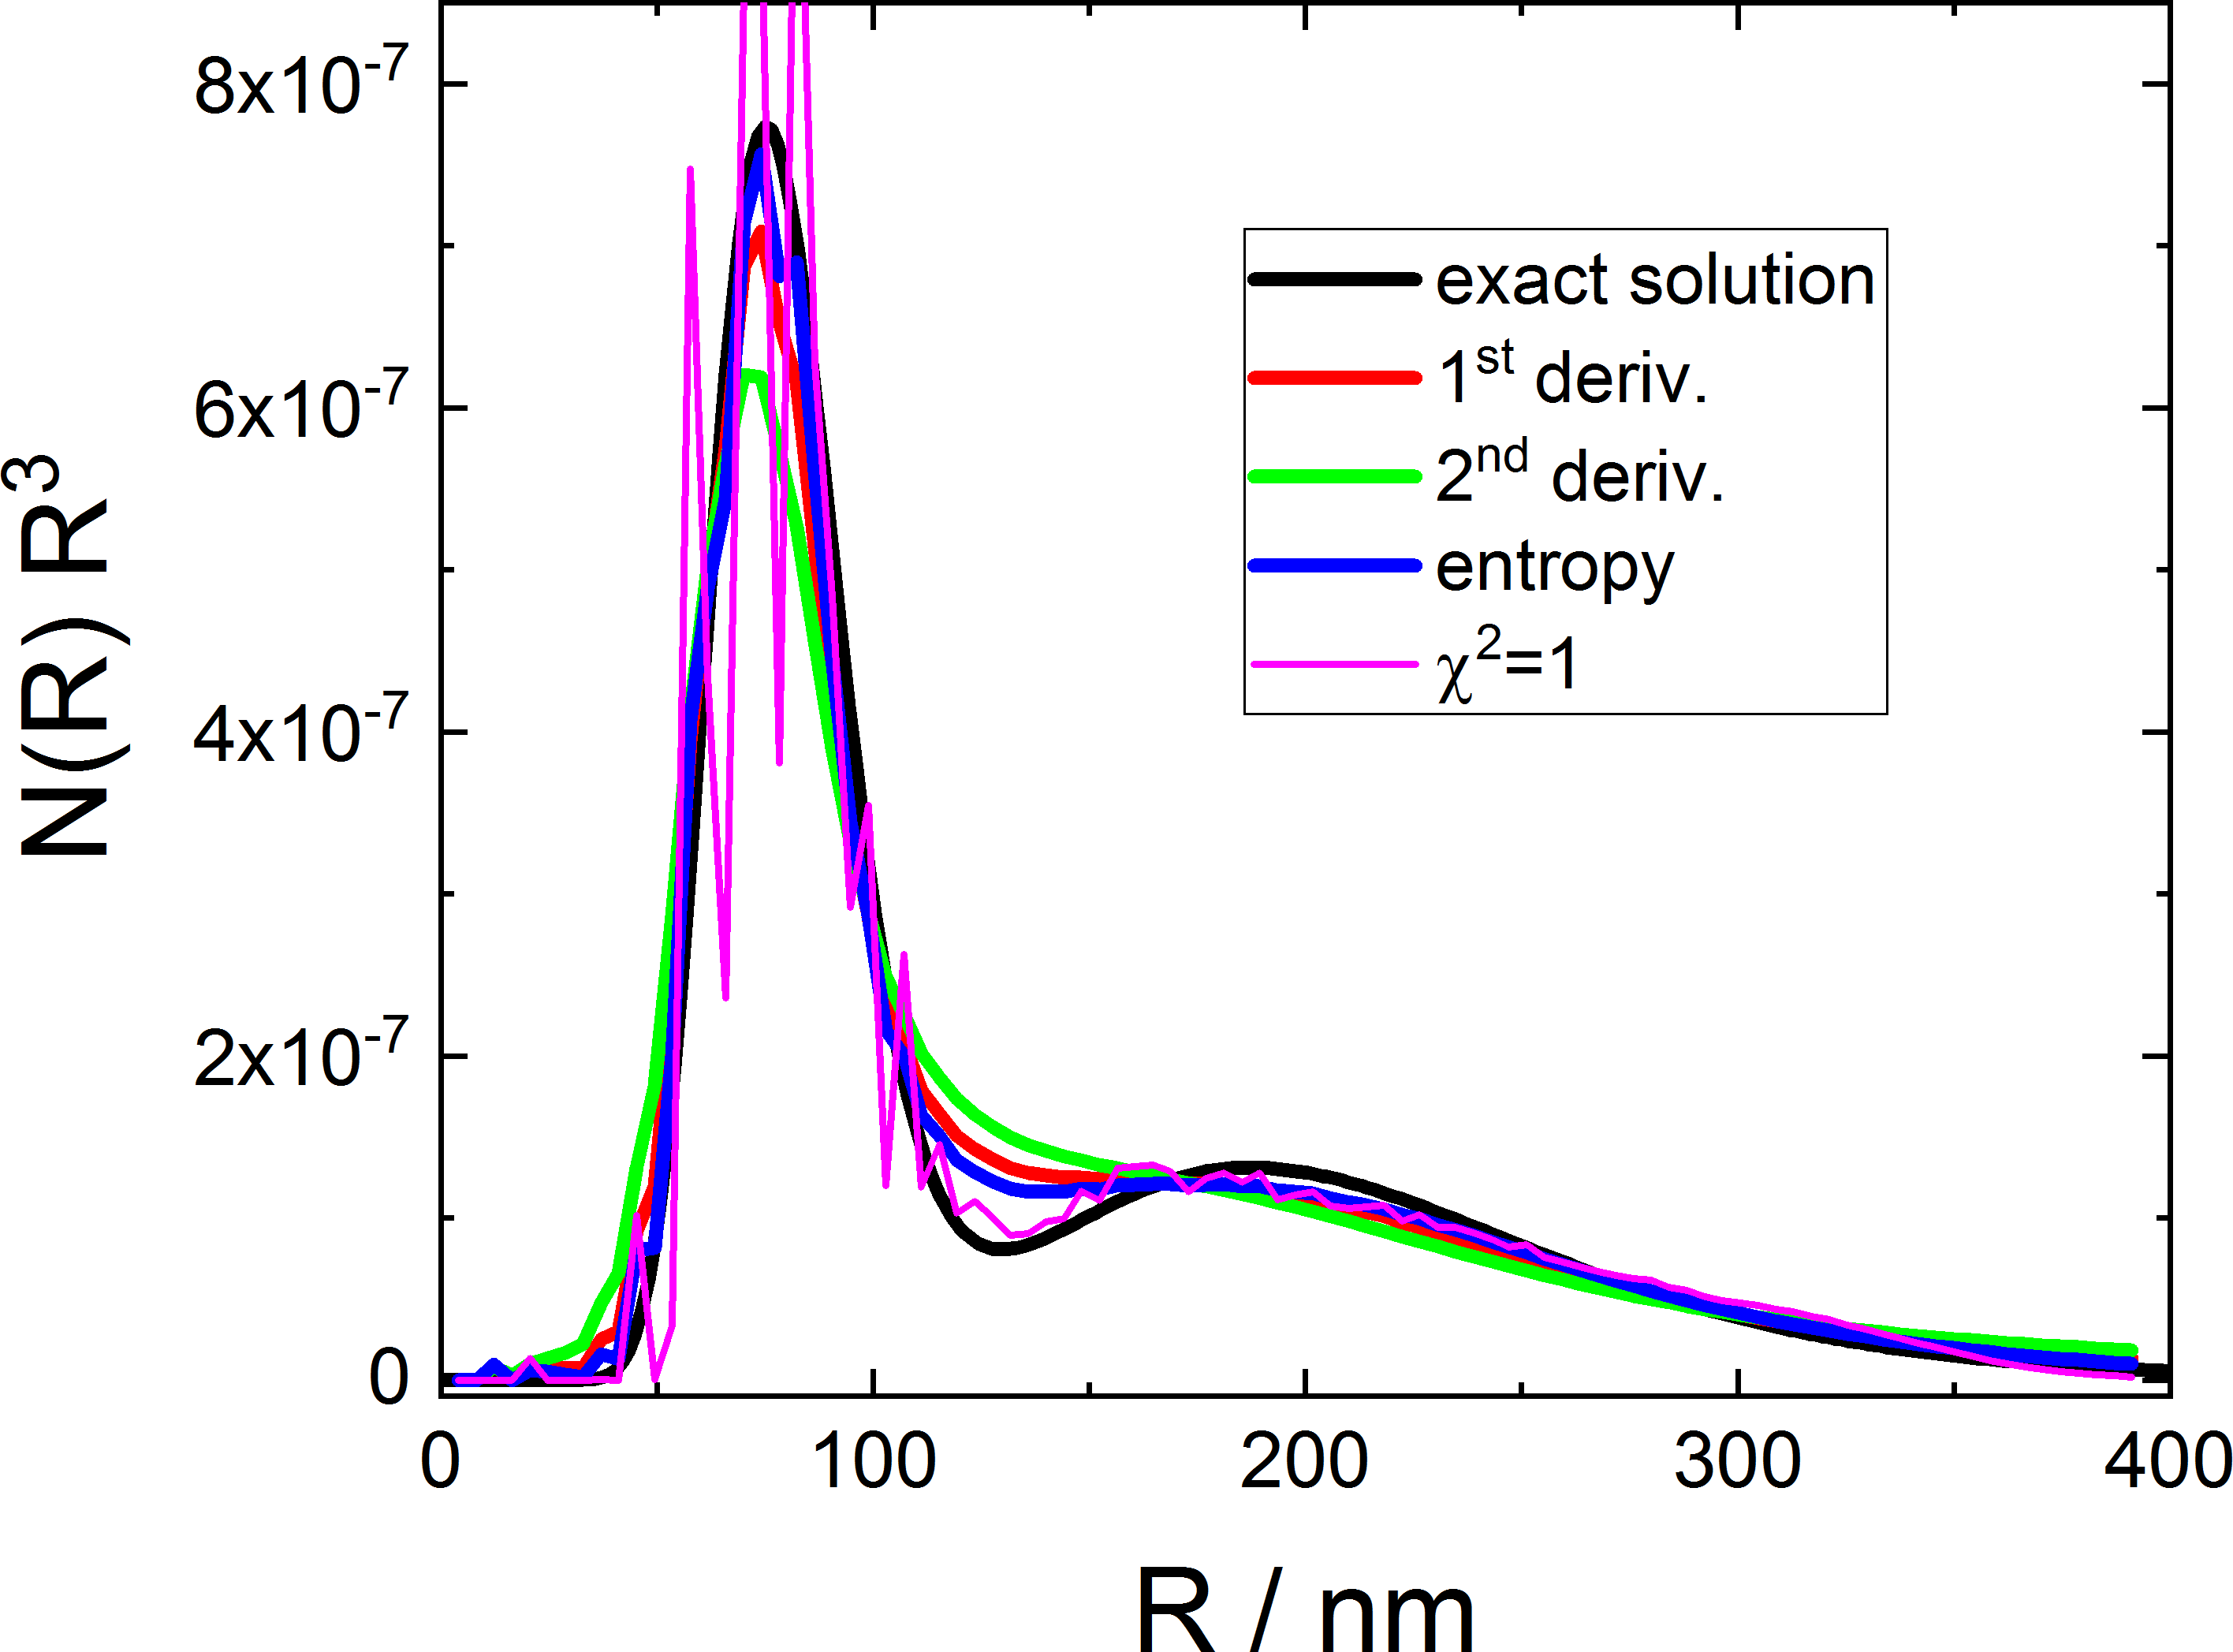
\includegraphics[width=0.42\textwidth]{../images/form_factor/EM/EMconstNRR3.png}\hspace{0.06\textwidth}
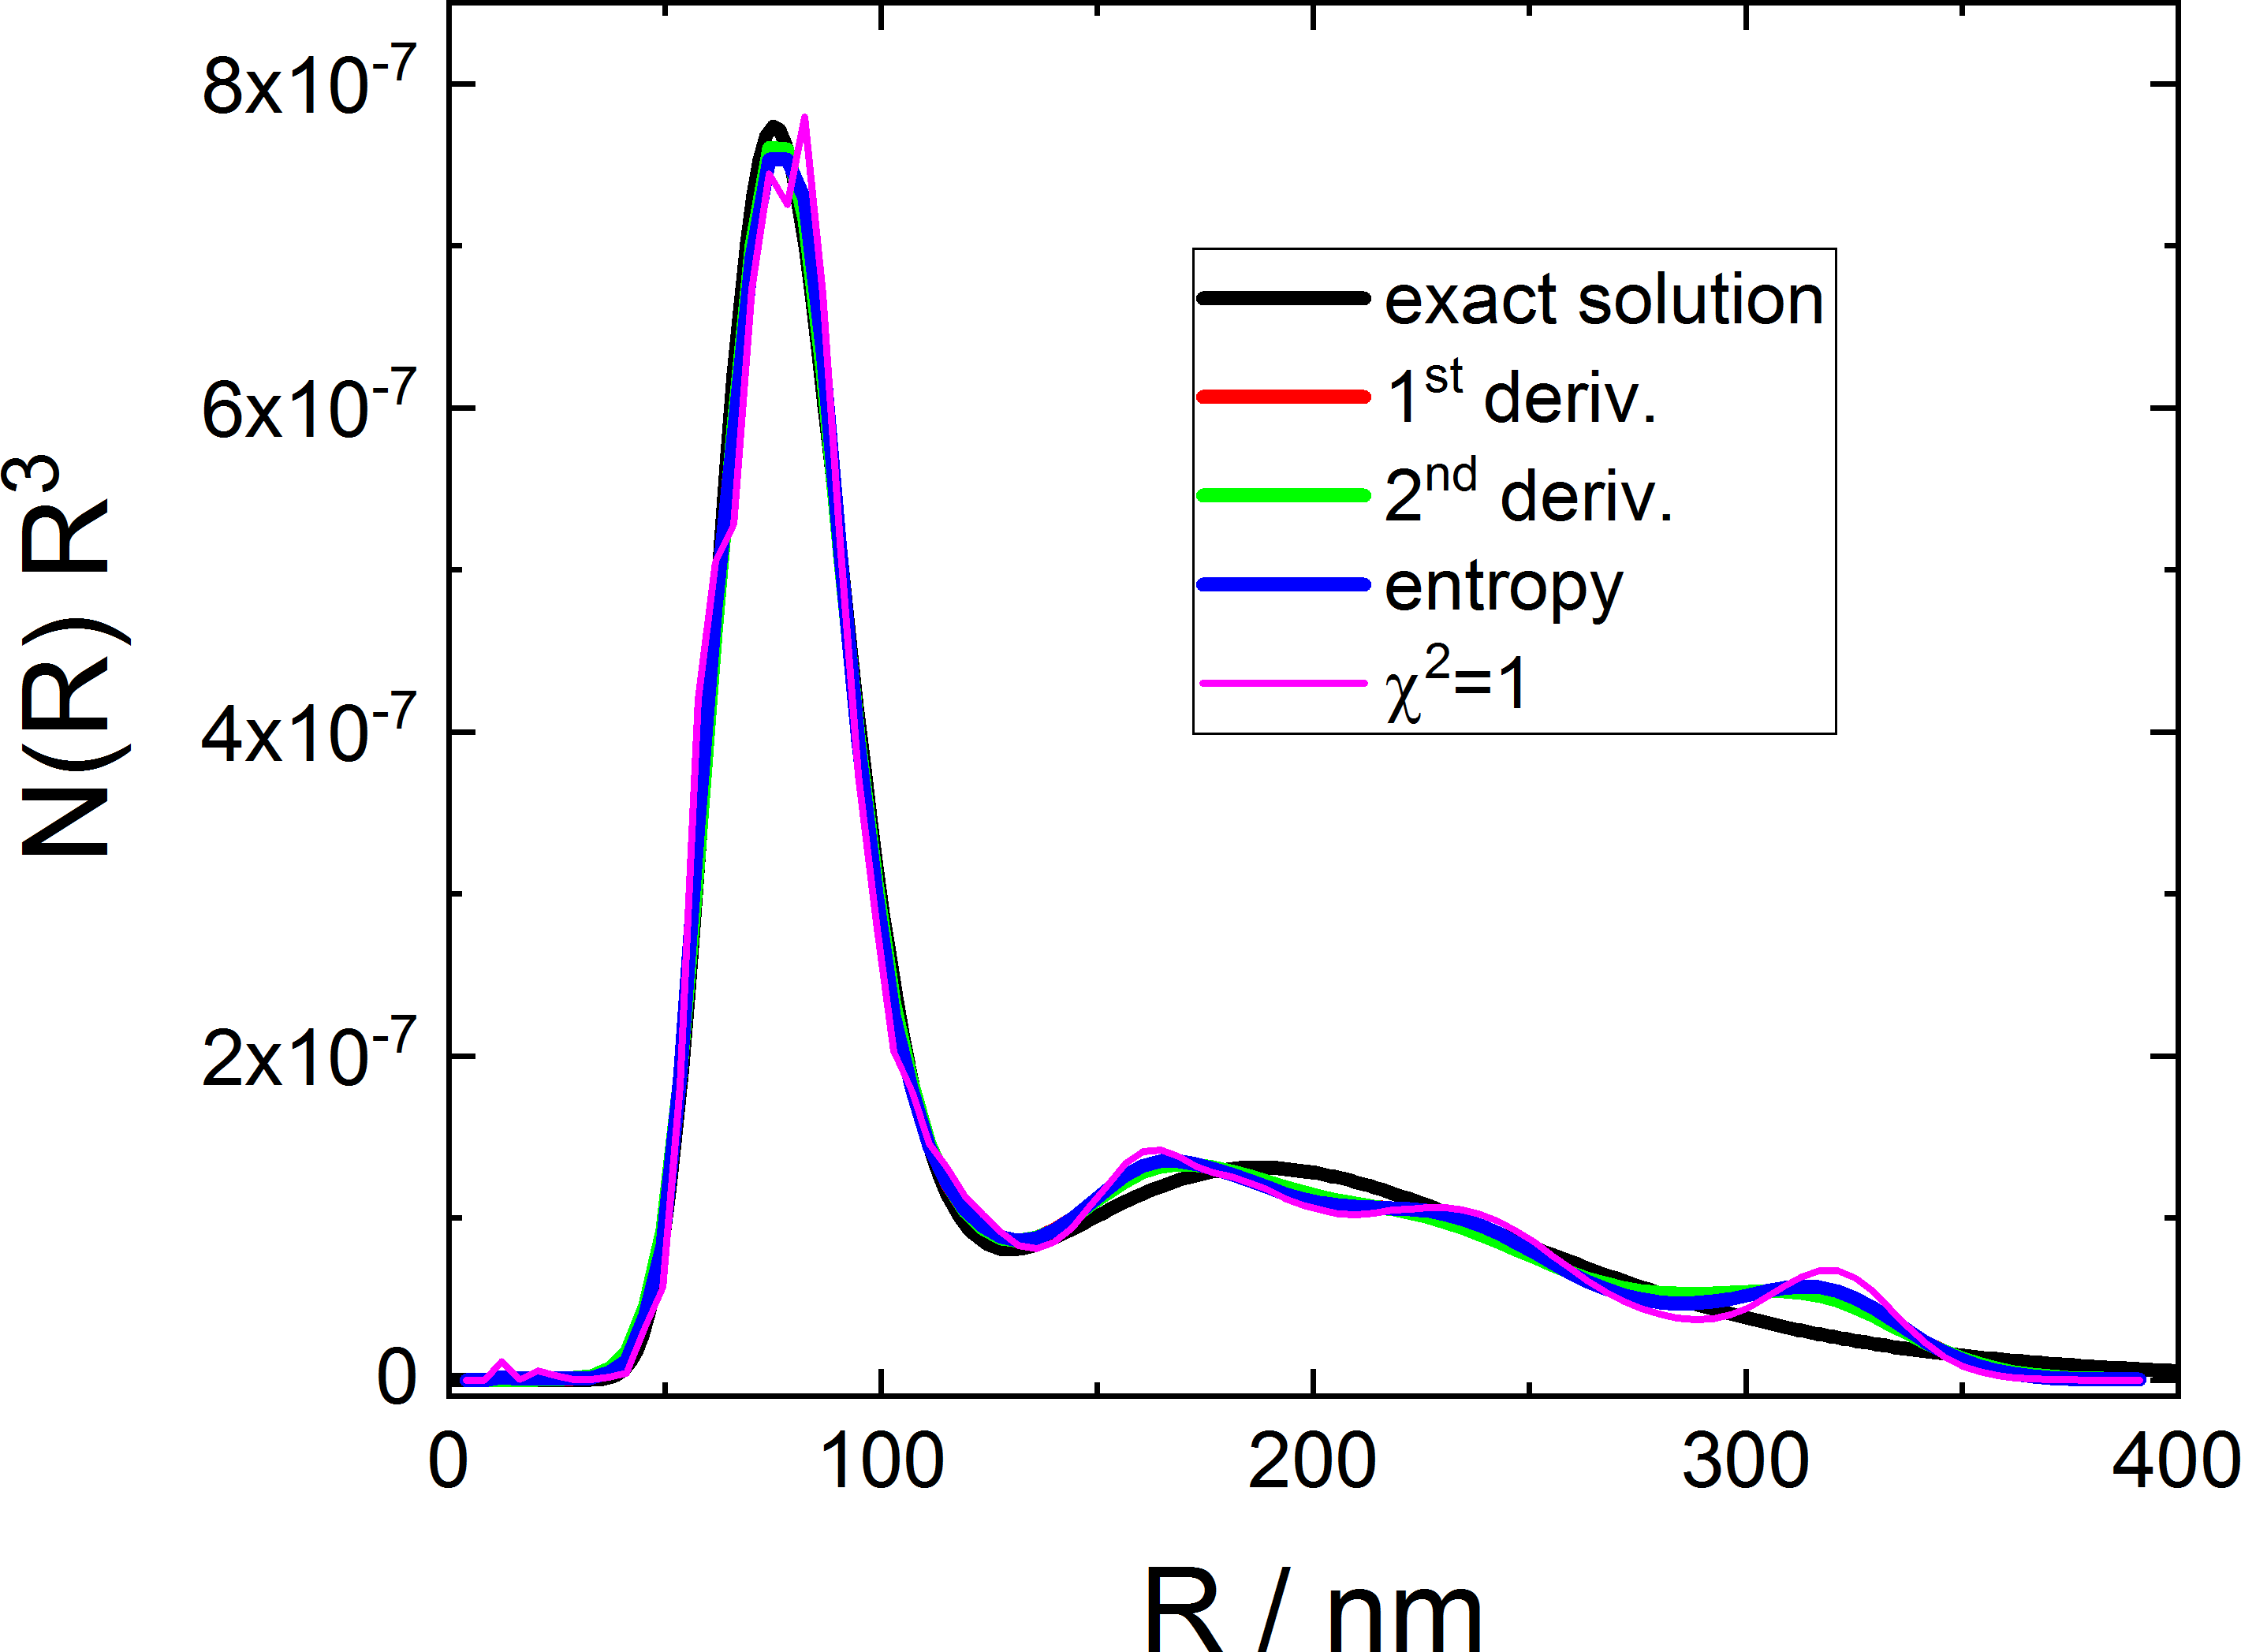
\includegraphics[width=0.42\textwidth]{../images/form_factor/EM/EMadaptiveNRR3.png}
\caption{The smoothing parameters has been obtained by the corners of the L-curves in fig.\ \ref{fig:EMlambdaLcurve} and the solution of the EM iteration scheme using Maximum Entropy term with constant and adaptive prior is compared with the exact solution as well as for a Lagrange parameter leading to weighted sum of squared residuals of $\chi_r^2=1$.\label{fig:EMconstadaptiveNRR3}}
\end{figure}


\subsection{Acceleration of EM iteration scheme} ~\\
There exist several very efficient algorithms to increase the convergence rate of contractive fixed point operators. A few of them are listed below.

 Lewitt et al.\ \cite{Lewitt1986} have suggested to increase the convergence rate by introducing an overrelaxation parameter in the iteration loop
\begin{align}\label{eq:OverRelaxation}
  x_j^{(k+1)} &= x_j^{(k)} + \lambda^{(k)}\Delta x_j^{(k)}
\end{align}
where $\lambda^{(k)}$ is the overrelaxation parameter $(\lambda^{(k)}> 1)$ whose
purpose is to accelerate the iterative process, and whose value is not so large as to violate the nonnegativity condition $x_j^{(k+1)} > 0$. To ensure that the overrelaxation of negative corrections to the solution vector does not decrease the value of any solution vector component below zero they suggest the following algorithm: first a pseudorelaxation parameter $\mu_j^{(k)}$ is calculated where
\begin{align}
\label{eq:pseudorelaxation}
  \mu_j^{(k)} &=
  \begin{cases}
    \infty, & \mbox{if } x_j^{(k)} \geq 0 \\
    \abs{\frac{x_j^{(k)}}{\Delta x_j^{(k)}}}, & \mbox{otherwise}.
  \end{cases}
\end{align}
Then they defined a critical relaxation parameter as follows:
\begin{align}\label{eq:criticalrelaxationparameter}
  \hat{\lambda}^{(k)} &= \min_j \mu_j^{(k)}
\end{align}
Finally the overrelaxation parameter $\lambda^{(k)}$ was chosen according to
\begin{align}\label{eq:useopverrelaxationparameter}
  \lambda^{(k)} &= \min \left[ \left(\hat{\lambda}^{(k)}-1\right)/2,\lambda^{\max}\right]
\end{align}
with $\lambda^{\max} \simeq 4$ so that $1\leq  \lambda^{(k)}\leq \lambda^{\max}$.

\begin{algorithm}[bht] \footnotesize
\caption{Biggs-Andrews vector extrapolation acceleration of order $o=0,1,2$ }\label{algorithm:Biggs_Andrews}
\begin{algorithmic}[1]
\Procedure{update\_vectors}{$\mathbf{g}^{(n-2)}$,$\mathbf{g}^{(n-1)}$,$\mathbf{x}^{(n+1)}$,$\mathbf{x}^{(n)}$,$\mathbf{x}^{(n-1)}$,$\mathbf{x}^{(n-2)}$}
    \State $\mathbf{g}^{(n-2)} \gets \mathbf{g}^{(n-1)}$
    \State $\mathbf{g}^{(n-1)} \gets \mathbf{x}^{(n+1)}-\mathbf{x}^{(n)}$
    \State $\mathbf{x}^{(n-2)} \gets \mathbf{x}^{(n-1)}$
    \State $\mathbf{x}^{(n-1)} \gets \mathbf{x}^{(n)}$
    \State $\mathbf{x}^{(n)} \gets \mathbf{x}^{(n+1)}$
\EndProcedure
\State \Comment Acceleration of the fixed point operator $\mathcal{O}[\mathbf{x}]=\mathbf{x}$
\Procedure{Biggs\_Andrews\_acceleration}{$\mathcal{O}[]$, $\mathbf{x}^{(0)}$, o}
\State $\alpha \gets 0$
\State $\mathbf{x}^{(n)} \gets \mathbf{x}^{(0)}$
\State $\mathbf{x}^{(n+1)} \gets \mathcal{O}[\mathbf{x}^{(n)}]$
\State \Call{update\_vectors}{$\mathbf{g}^{(n-2)}$,$\mathbf{g}^{(n-1)}$,$\mathbf{x}^{(n+1)}$,$\mathbf{x}^{(n)}$,$\mathbf{x}^{(n-1)}$,$\mathbf{x}^{(n-2)}$}
\State $\mathbf{x}^{(n+1)} \gets \mathcal{O}[\mathbf{x}^{(n)}]$
\State \Call{update\_vectors}{$\mathbf{g}^{(n-2)}$,$\mathbf{g}^{(n-1)}$,$\mathbf{x}^{(n+1)}$,$\mathbf{x}^{(n)}$,$\mathbf{x}^{(n-1)}$,$\mathbf{x}^{(n-2)}$}
\State $\mathbf{y}^{(n)} \gets  \mathbf{x}^{(n+1)}$
\While{($\mathcal{O}[]$ not converged)}
    \State \Comment $\alpha$ needs to be updated first
    \State $\alpha = \frac{\left(\mathbf{g}^{(n-1)}\right)^T\mathbf{g}^{(n-2)}}{\left(\mathbf{g}^{(n-2)}\right)^T\mathbf{g}^{(n-2)}}$
    \State $\alpha \gets \max (\min (\alpha,1),0)$
    \State $\mathbf{x}^{(n+1)} \gets \mathcal{O}[\mathbf{y}^{(n)}]$
    \State \Comment  guess of next virtual step $\mathbf{y}^{(n)}$ calculated up to $o^\mathrm{th}$-order
    \If{$\alpha = 0 \wedge o=0$}
        \State $\mathbf{y}^{(n)} \gets \mathbf{x}^{(n)}$
    \ElsIf {$\alpha > 0 \vee o=1$}
        \State $\mathbf{y}^{(n)} \gets \mathbf{x}^{(n)} + \alpha \left(\mathbf{x}^{(n)}-\mathbf{x}^{(n-1)}\right)$
    \Else
        \State $\mathbf{y}^{(n)} \gets \mathbf{x}^{(n)}\mathbf{x}^{(n)} + \alpha \left(\mathbf{x}^{(n)}-\mathbf{x}^{(n-1)}\right)
                                                                        + \frac{\alpha^2}{2}\left(\mathbf{x}^{(n)}+2\mathbf{x}^{(n-1)}-\mathbf{x}^{(n-2)}\right)$
    \EndIf
    \State \Comment now all the other temporary vectors are updated
    \State \Call{update\_vectors}{$\mathbf{g}^{(n-2)}$,$\mathbf{g}^{(n-1)}$,$\mathbf{x}^{(n+1)}$,$\mathbf{x}^{(n)}$,$\mathbf{x}^{(n-1)}$,$\mathbf{x}^{(n-2)}$}

\EndWhile
\EndProcedure
\end{algorithmic}
\end{algorithm}

Another more efficient method to accelerate the convergence rate of the EM iteration scheme is the so called Anderson acceleration \cite{Anderson1965} to solve fixed point problems (see also \cite{Walker2011,Toth2015}), which also has been suggested for the EM iteration scheme \cite{Henderson2019}. In \SASfit several fixed point accelerations are supplied by making use of the sundials library \cite{Hindmarsh2005}. However, only the supplied Anderson acceleration speeds up the fixed point iterations whereas all the others like GMRES \cite{Saad1986}, FGMRES \cite{Saad1993}, Bi-CGStab \cite{Vorst1992} or TFQMR \cite{Freund1993} become instable and do not converge.

In \cite{Biggs1997, Biggs1995, Biggs1998, Wang2014,Jiang2017} an acceleration process has been suggested basing on vector extrapolation which does not require an extra evaluation of the fixed point operator $\mathcal{O}_\mathrm{EM}$ in eq.\ \ref{eq:LucyRichardsonInversionMethod}. The method just needs to remember one or two previous solution vectors for calculating either the first or additionally the second derivative for guessing the next virtual solution vector, which is then used as an input vector for the next step of the fixed point iteration. The algorithm is described in alg.\ \ref{algorithm:Biggs_Andrews}. The convergence behaviour of the different acceleration schemes are shown in fig.\ \ref{fig:EMconvergenceSpeed}. Quite good acceleration has been achieved by the Biggs-Andrews method as well as Anderson acceleration, whereas other classical methods like GMRES, Bi-CGSab or TFQMR failed. The Picard iteration scheme and  overrelaxation method need orders of magnitudes more iterations to reach the true fixed point solution. The preferred acceleration scheme therefore becomes the Biggs-Andrews methods.


\begin{figure}[htb]
\centering
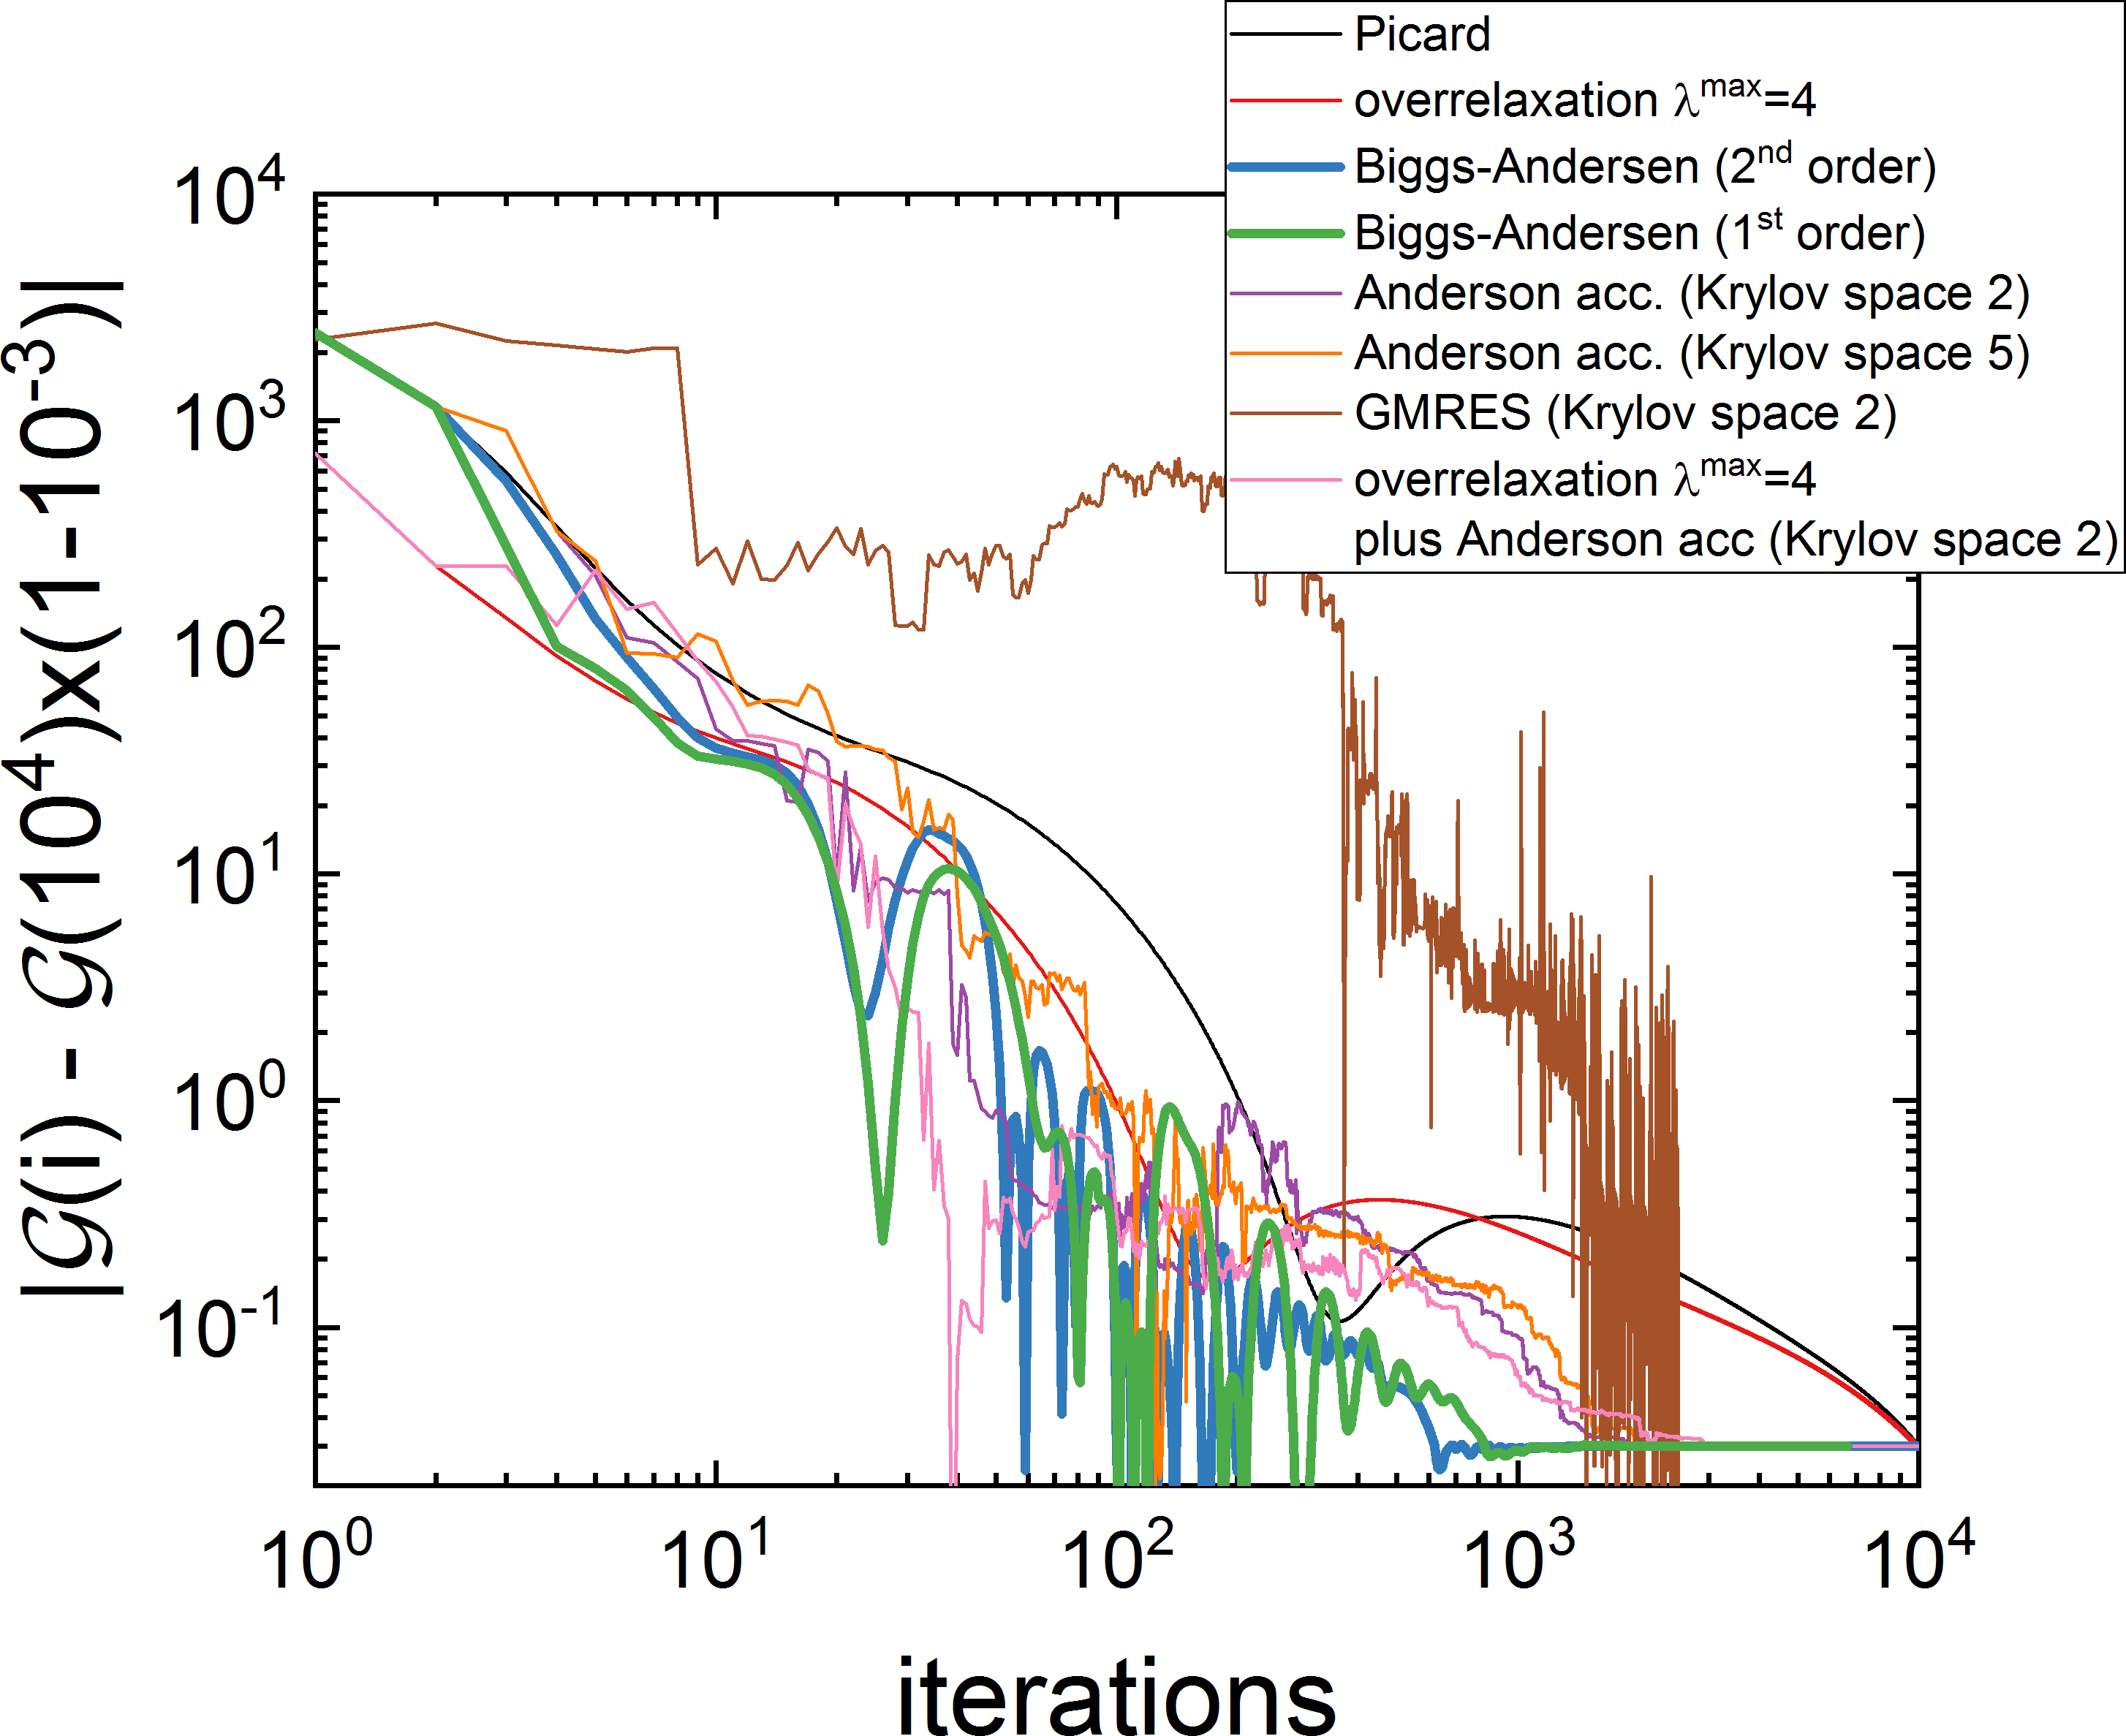
\includegraphics[width=0.62\textwidth]{../images/form_factor/EM/EMconvergenceSpeed.png}
\caption{Convergence behaviour of a few acceleration schemes compared to the non-accelerated Picard iteration.\label{fig:EMconvergenceSpeed}}
\end{figure}

\section{Linear least square regularization (LLS)}
\label{sec:LLS}
Linear least square regularization has been implemented using the GNU scientific library (\texttt{gsl}). It supplies routines to solve ill-posed problems including a regularization term in the least squares minimization
\begin{align}\label{eq:LLSreg}
  \chi^2 &= || \mathbf{b} - \hat{\mathbf{A}}\mathbf{x} ||_{w}^2 + \lambda^2 || \hat{\mathbf{L}} \mathbf{x} ||^2
\end{align}
Here $|| \dots ||_{w}^2$ denotes the weighted sum of squared residuals
\begin{align}\label{eq:wSumSR}
\left\| \hat{\mathbf{A}}\mathbf{x}-\mathbf{b}\right\|_W^2
&= \left(\mathbf{x}^T\hat{\mathbf{A}}^T\hat{\mathbf{w}}^T-\mathbf{b}^T\hat{\mathbf{w}}^T\right)\left(\hat{\mathbf{w}}\hat{\mathbf{A}}\mathbf{x}-\hat{\mathbf{w}}\mathbf{b}\right)\\
&= \mathbf{x}^T\hat{\mathbf{A}}^T\hat{\mathbf{w}}^T\hat{\mathbf{w}}\hat{\mathbf{A}}\mathbf{x}-2 \mathbf{x}^T\hat{\mathbf{A}}^T\hat{\mathbf{w}}^T\hat{\mathbf{w}}\mathbf{b}+\mathbf{b}^T\hat{\mathbf{w}}^T\hat{\mathbf{w}}\mathbf{b}
\end{align}
with
\begin{align}
  \hat{\mathbf{w}} &=
  \begin{pmatrix}
    \frac{1}{\Delta b_0} & 0 & \dots & 0 \\
    0 & \frac{1}{\Delta b_1} & \dots & 0 \\
    \vdots & \vdots & \ddots & \vdots \\
    0 & 0 & \dots & \frac{1}{\Delta b_{M-1}}
  \end{pmatrix}
\end{align}
where $\Delta b_i$ are the experimental errors (standard deviation, Gaussian error or root-mean-square error) of the measured quantities $b_i$.
$\hat{\mathbf{L}}$ describes the penalty contribution and $\lambda$
 is the regularization parameter. To determine a suitable value for it automatically several routines are supplied in the \texttt{gsl} library. Several choices for the penalty term $\hat{\mathbf{L}}$ are supplied
 In the simplest case the penalty term is the identity matrix $\hat{\mathbf{L}} = \hat{\mathbf{I}}$ so that the overall length of the solution vector is also tried to be minimized. As a second choice for the penalty term is the first-order discrete derivative operator \cite{Donatelli2014}
 \begin{align}\label{eq:first_derivative_penalty}
   \hat{\mathbf{L}}_\mathrm{1^{st}} &=
  \begin{pmatrix}
    -1    & 1      &        &  \\
          & \ddots & \ddots &  \\
          &        & -1     & 1
  \end{pmatrix} \in \mathbb{R}^{(N-1)\times N}
\end{align}
Since nonsingular regularization matrices are easier to handle than singular
ones a common approach is to use small perturbations.
If the perturbation is small enough the smoothing property is not deteriorated
significantly. With a small diagonal element $\epsilon > 0$
\begin{align}\label{eq:first_derivative_penalty_plus_epsilon}
   \hat{\mathbf{L}}_\mathrm{1^{st}} &=
  \begin{pmatrix}
  \epsilon & & & \\
    -1    & 1      &        &  \\
          & \ddots & \ddots &  \\
          &        & -1     & 1
  \end{pmatrix} \mbox{ or }  \hat{\mathbf{L}}_\mathrm{1^{st}}  =
  \begin{pmatrix}
    -1    & 1      &        &  \\
          & \ddots & \ddots &  \\
          &        & -1     & 1 \\
          & & & \epsilon \\
  \end{pmatrix} \in \mathbb{R}^{N\times N}
\end{align}
The additional element $\epsilon$ forces either the
first or last element to have small magnitude.
A further common regularization matrix is the discrete second-order derivative \cite{Donatelli2014}
operator
 \begin{align}\label{eq:second_derivative_penalty}
   \hat{\mathbf{L}}_\mathrm{2^{n}} &=
  \begin{pmatrix}
    -1    &  2     & -1     &        &  \\
          & \ddots & \ddots & \ddots &  \\
          &        & -1     & 2      & -1
  \end{pmatrix} \in \mathbb{R}^{(N-2)\times N}
\end{align}
Also for this case a nonsingular squared matrix can be used as an approximation by adding one row at the top and one row at the bottom and assuming either Dirichlet boundary conditions or Neumann boundary conditions
\begin{align}\label{eq:second_derivative_penalty_plus_DrichletNeumann}
   \hat{\mathbf{L}}_\mathrm{2^{nd}}^\mathrm{DD} &=
  \begin{pmatrix}
    2   & -1     &        &        &    \\
    -1  & 2      & -1     &        &    \\
        & \ddots & \ddots & \ddots &    \\
        &        &  -1    & 2      & -1 \\
        &        &        & -1     & 2  \\
  \end{pmatrix}  \in \mathbb{R}^{N\times N}\\
  \mbox{or}  \nonumber \\
  \hat{\mathbf{L}}_\mathrm{2^{nd}}^\mathrm{NN}  &=
  \begin{pmatrix}
     1  & -1     &        &        &  \\
    -1  & 2      & -1     &        &  \\
        & \ddots & \ddots & \ddots &  \\
        &        & -1     &  2     & -1 \\
        &        &        & -1     & 1  \\
  \end{pmatrix} \in \mathbb{R}^{N\times N}
\end{align}
Also mixed boundary condition with Dirichlet boundary condition at the left end point and the Neumann boundary condition at the
right one or  vice versa.
\begin{align}\label{eq:second_derivative_penalty_plus_mixedDrichletNeumann}
  \hat{\mathbf{L}}_\mathrm{2^{nd}}^\mathrm{ND}  &=
  \begin{pmatrix}
    2   & -1     &        &        &    \\
    -1  & 2      & -1     &        &    \\
        & \ddots & \ddots & \ddots &    \\
        &        & -1     &  2     & -1 \\
        &        &        & -1     &  1
  \end{pmatrix} \in \mathbb{R}^{N\times N} \\
  \mbox{or}  \nonumber\\
   \hat{\mathbf{L}}_\mathrm{2^{nd}}^\mathrm{DN} &=
  \begin{pmatrix}
     1  & -1     &        &        &    \\
    -1  & 2      &  -1    &        &    \\
        & \ddots & \ddots & \ddots &    \\
        &        &  -1    &  2     & -1 \\
        &        &        & -1     & 2
  \end{pmatrix}  \in \mathbb{R}^{N\times N}
\end{align}

\begin{figure}[htb]
\centering
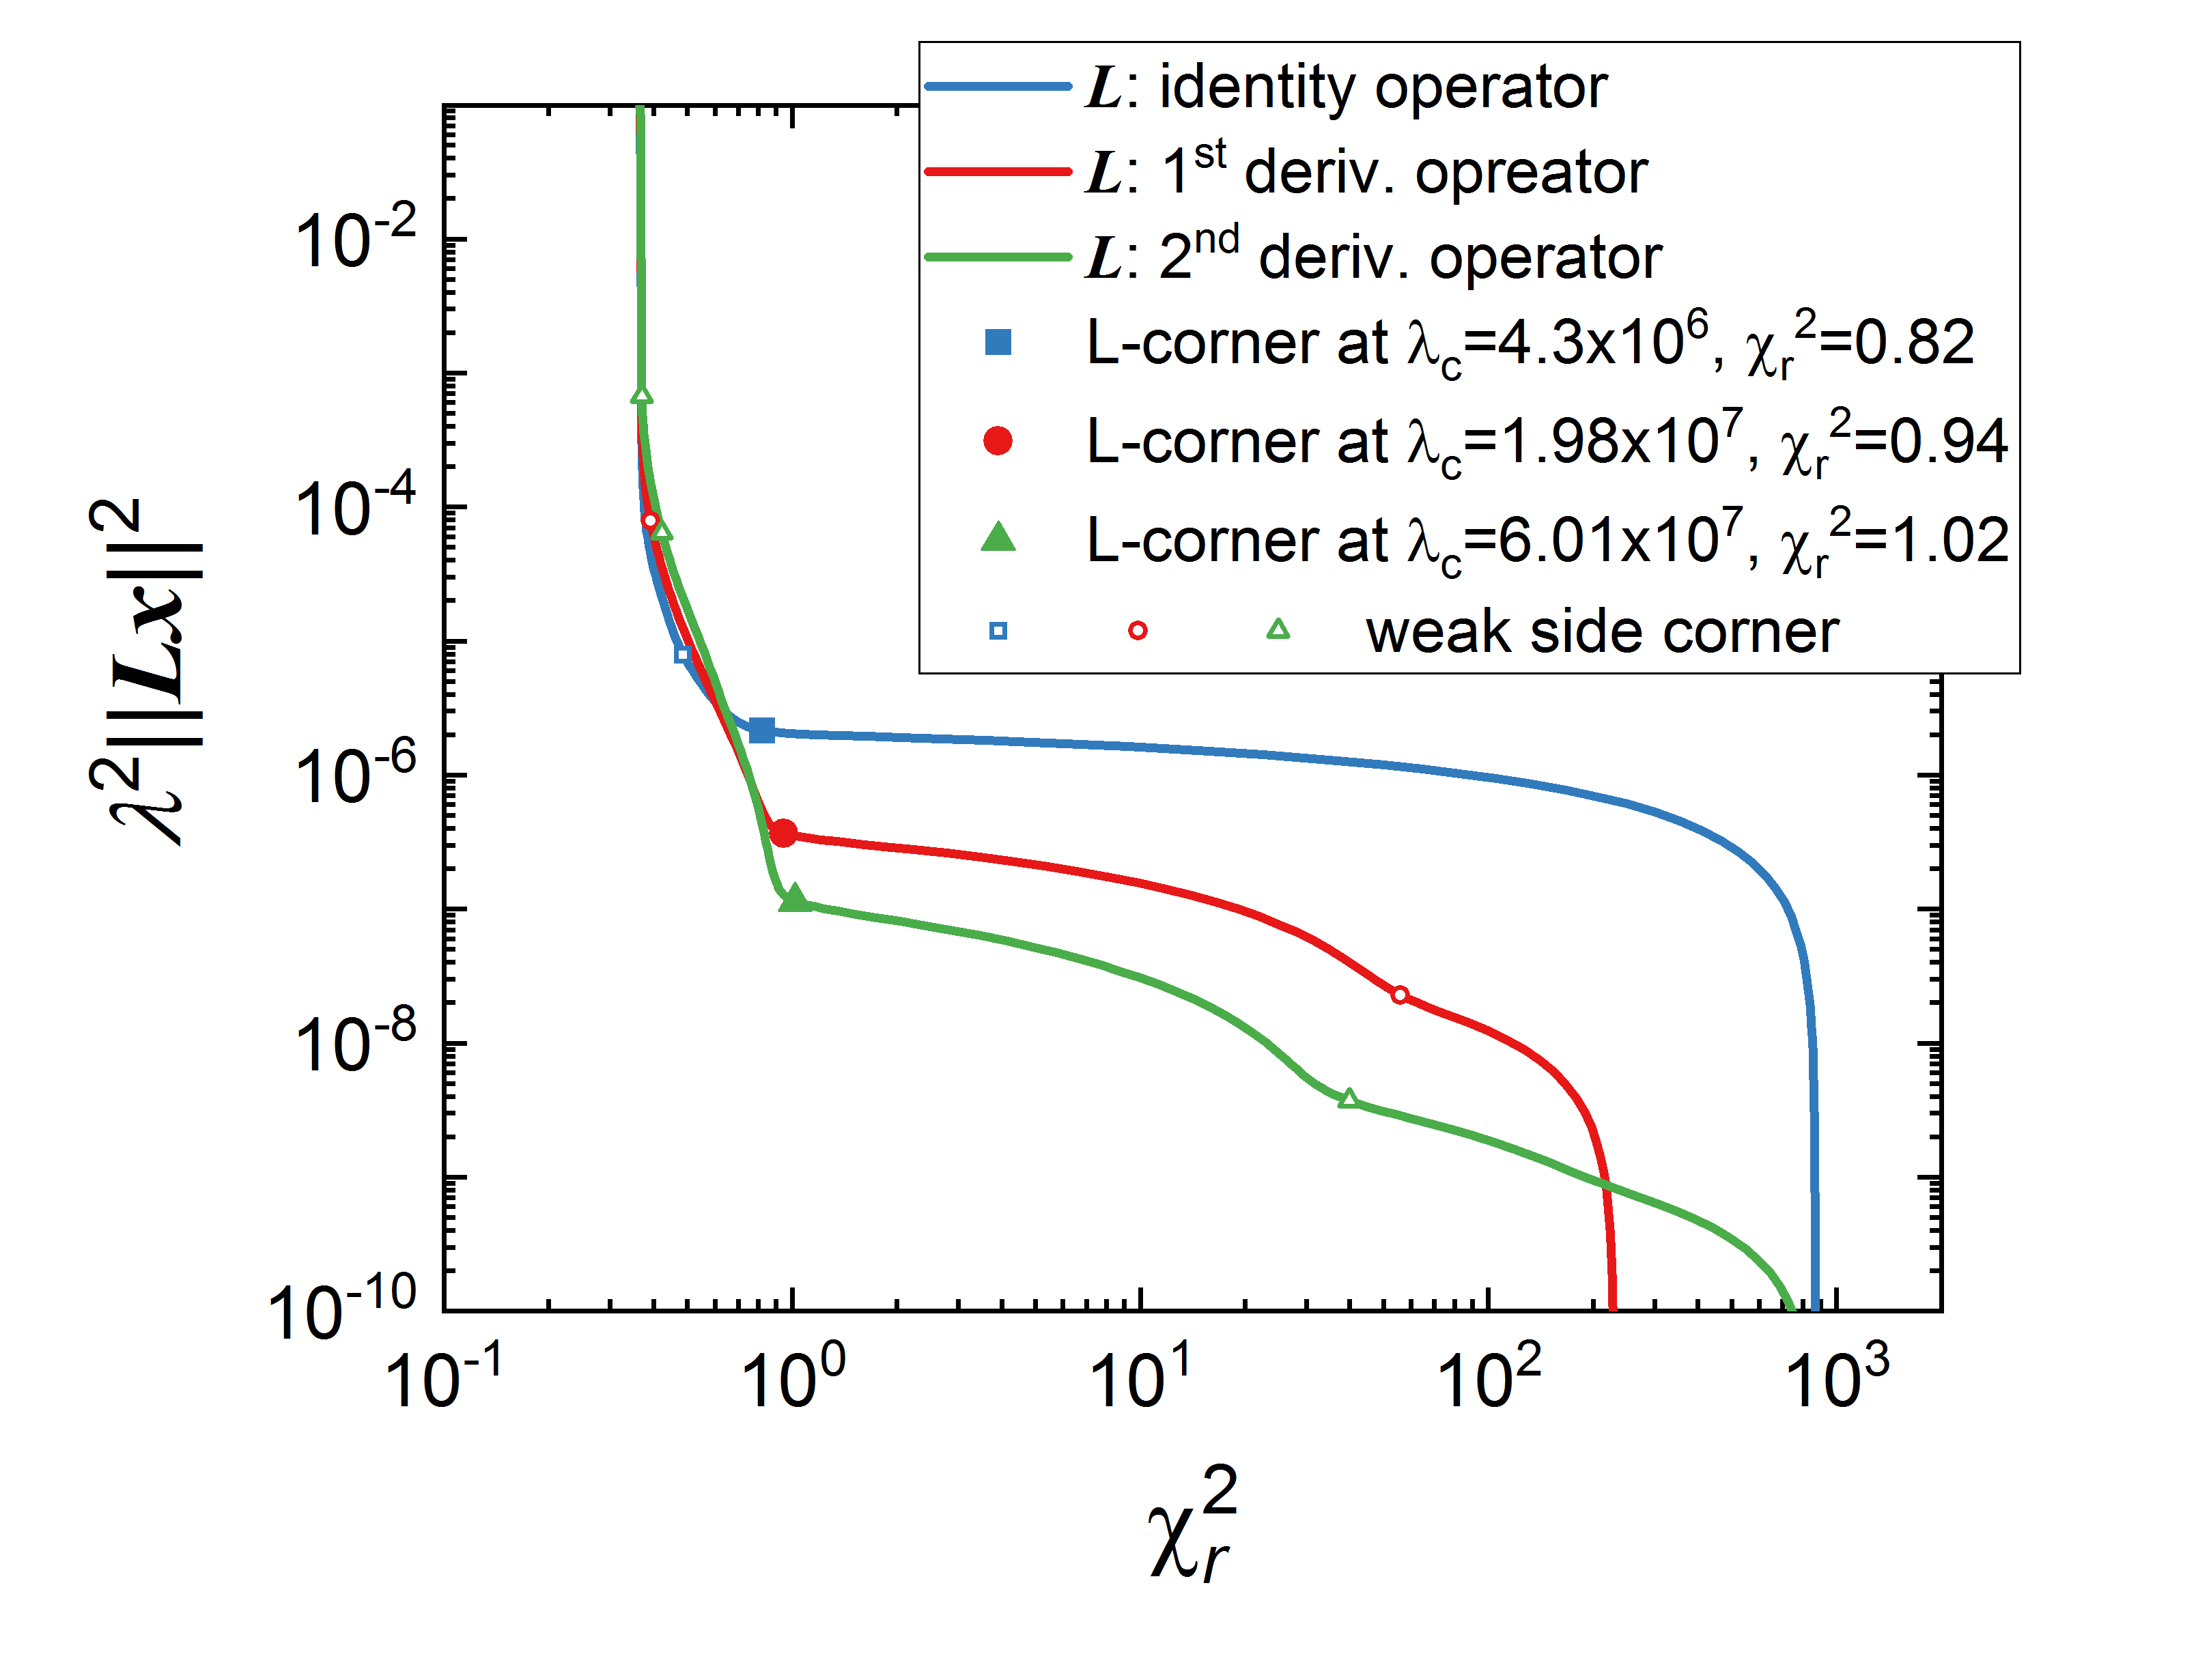
\includegraphics[width=0.45\textwidth]{../images/form_factor/EM/LLS_Lcorner.png}\hspace{0.02\textwidth}
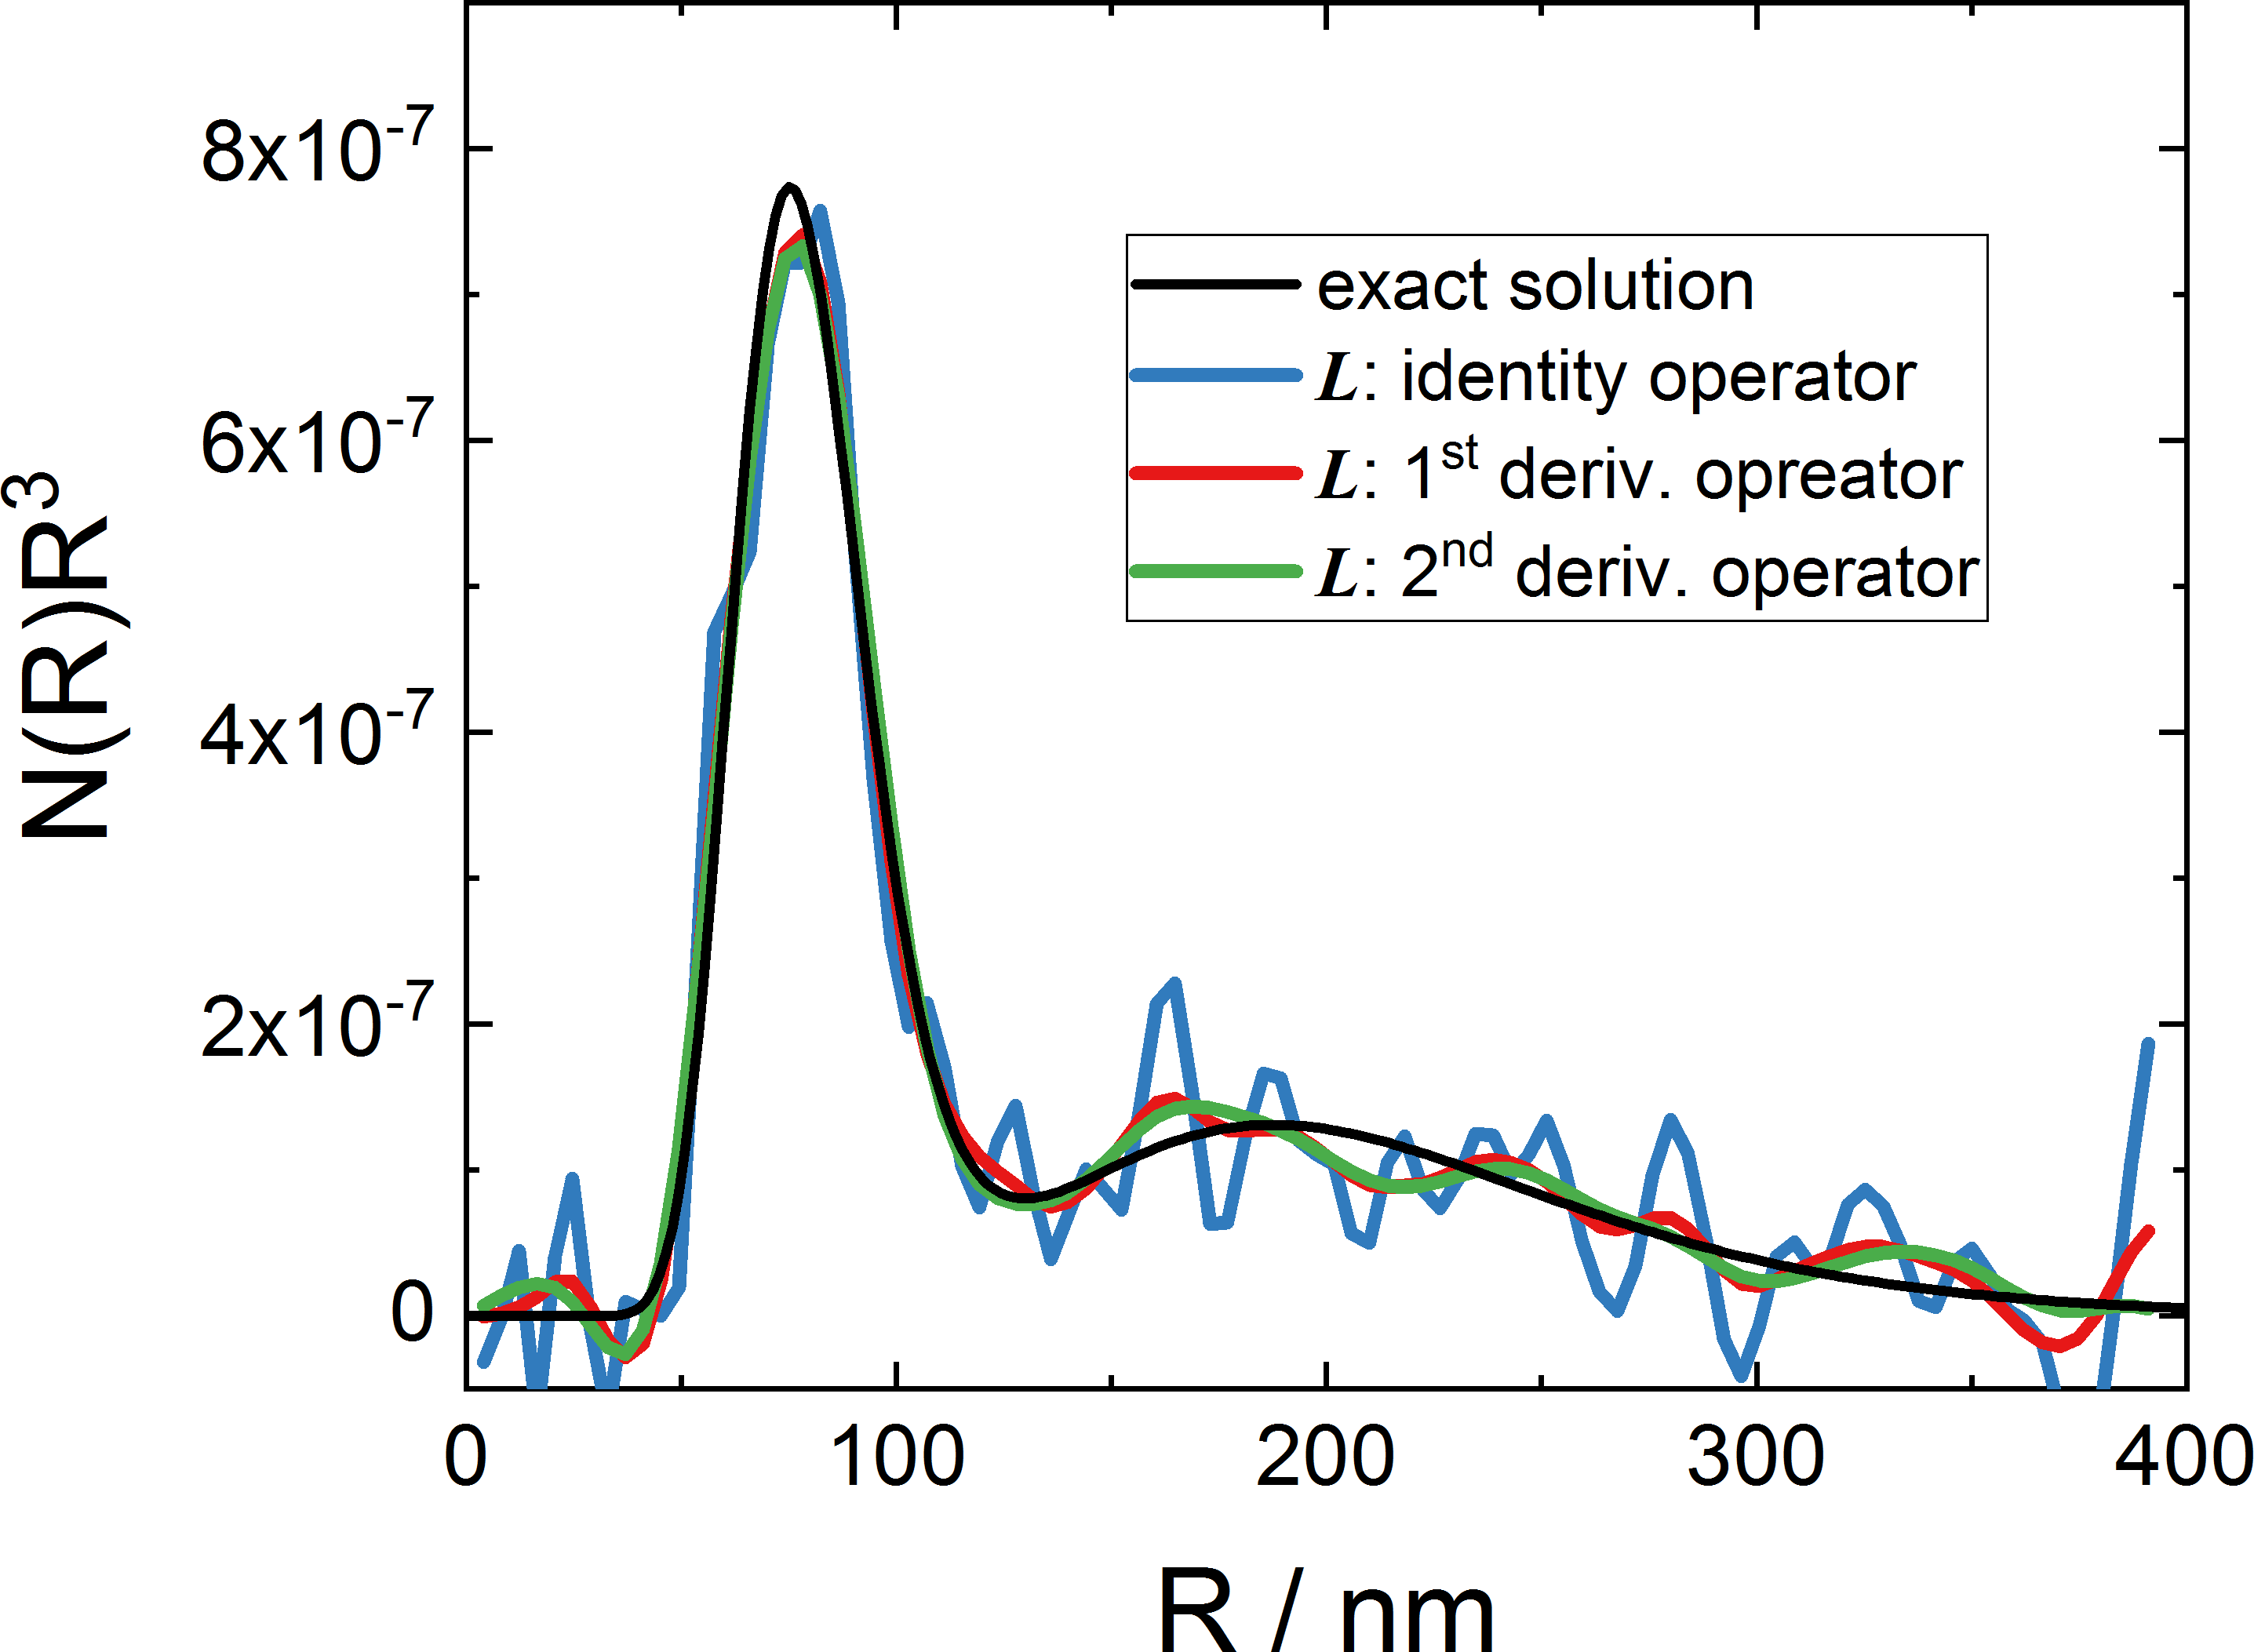
\includegraphics[width=0.45\textwidth]{../images/form_factor/EM/LLS_NRR3_Lcorner.png}
\caption{The optimum Lagrange parameters $\lambda_c$ have been obtained by the corners of the L-curves for $\hat{\mathbf{L}}=\hat{\mathbf{1}}$, $\hat{\mathbf{L}}=\hat{\mathbf{L}}_\mathrm{1^{st}}$ and $\hat{\mathbf{L}}=\hat{\mathbf{L}}_\mathrm{2^{nd}}$. \label{fig:EMLcorner}}
\end{figure}

\begin{figure}[htb]
\centering
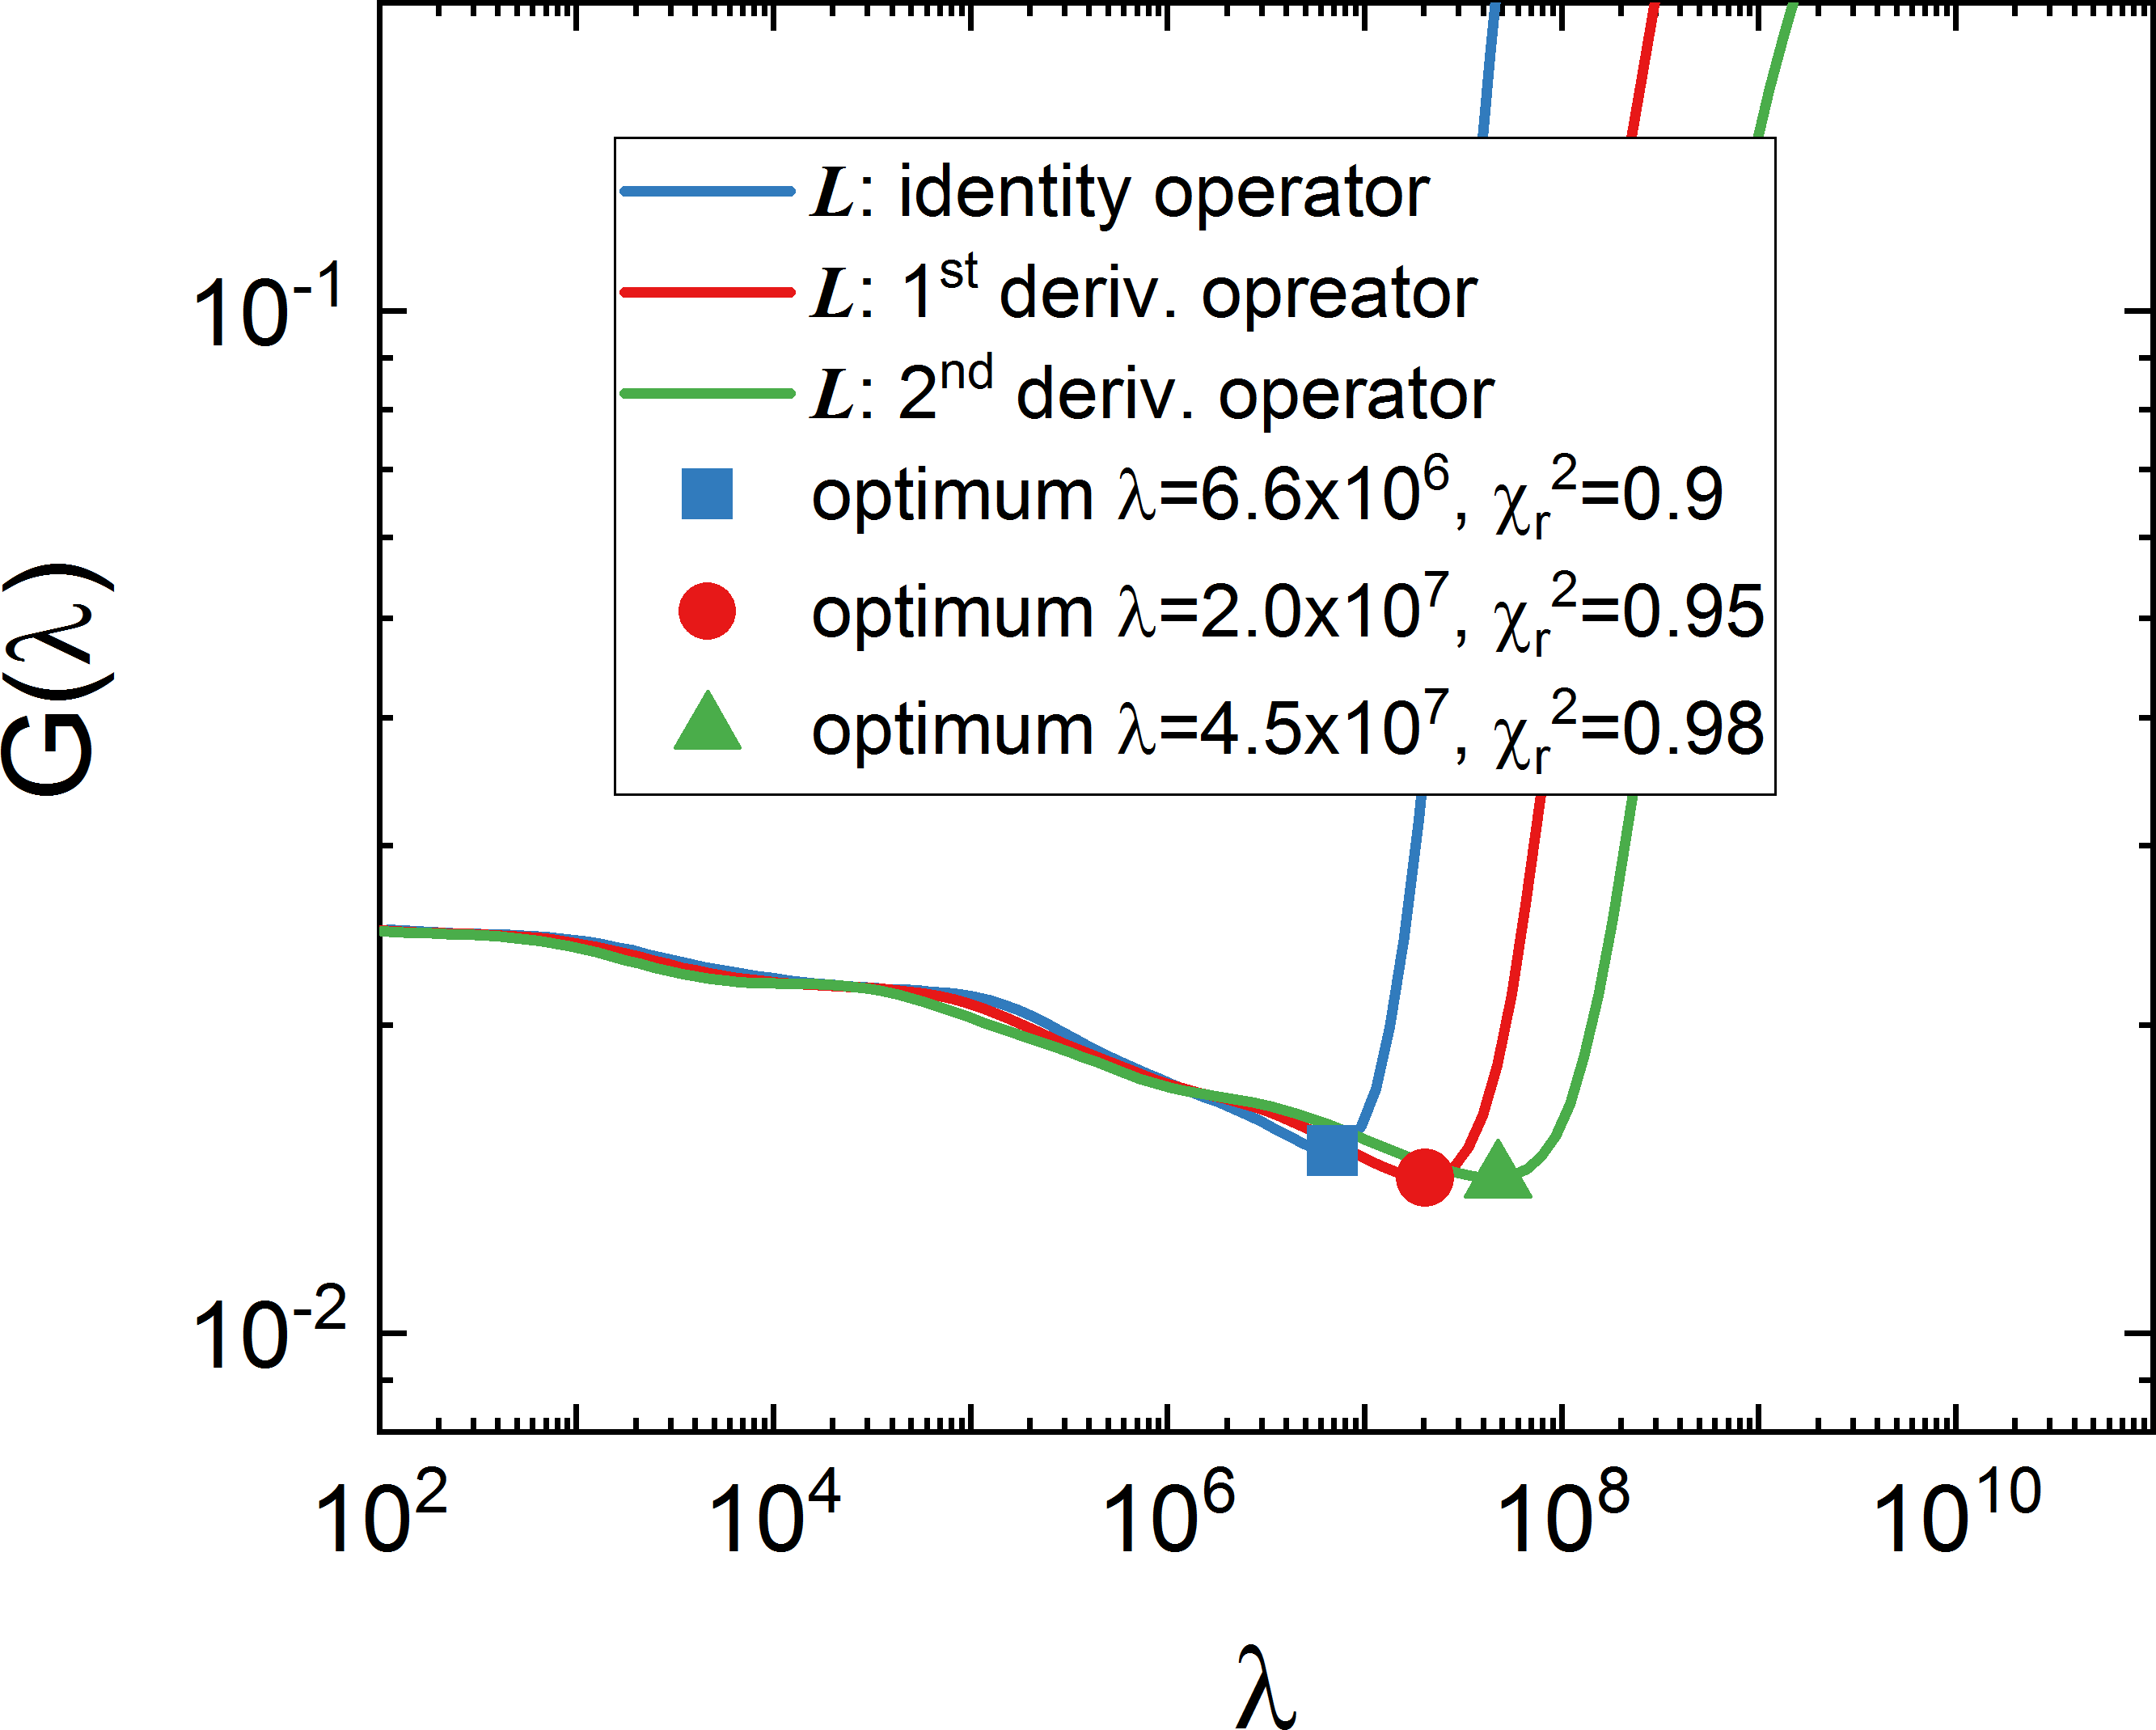
\includegraphics[width=0.42\textwidth]{../images/form_factor/EM/LLS_GCVcurve.png}\hspace{0.05\textwidth}
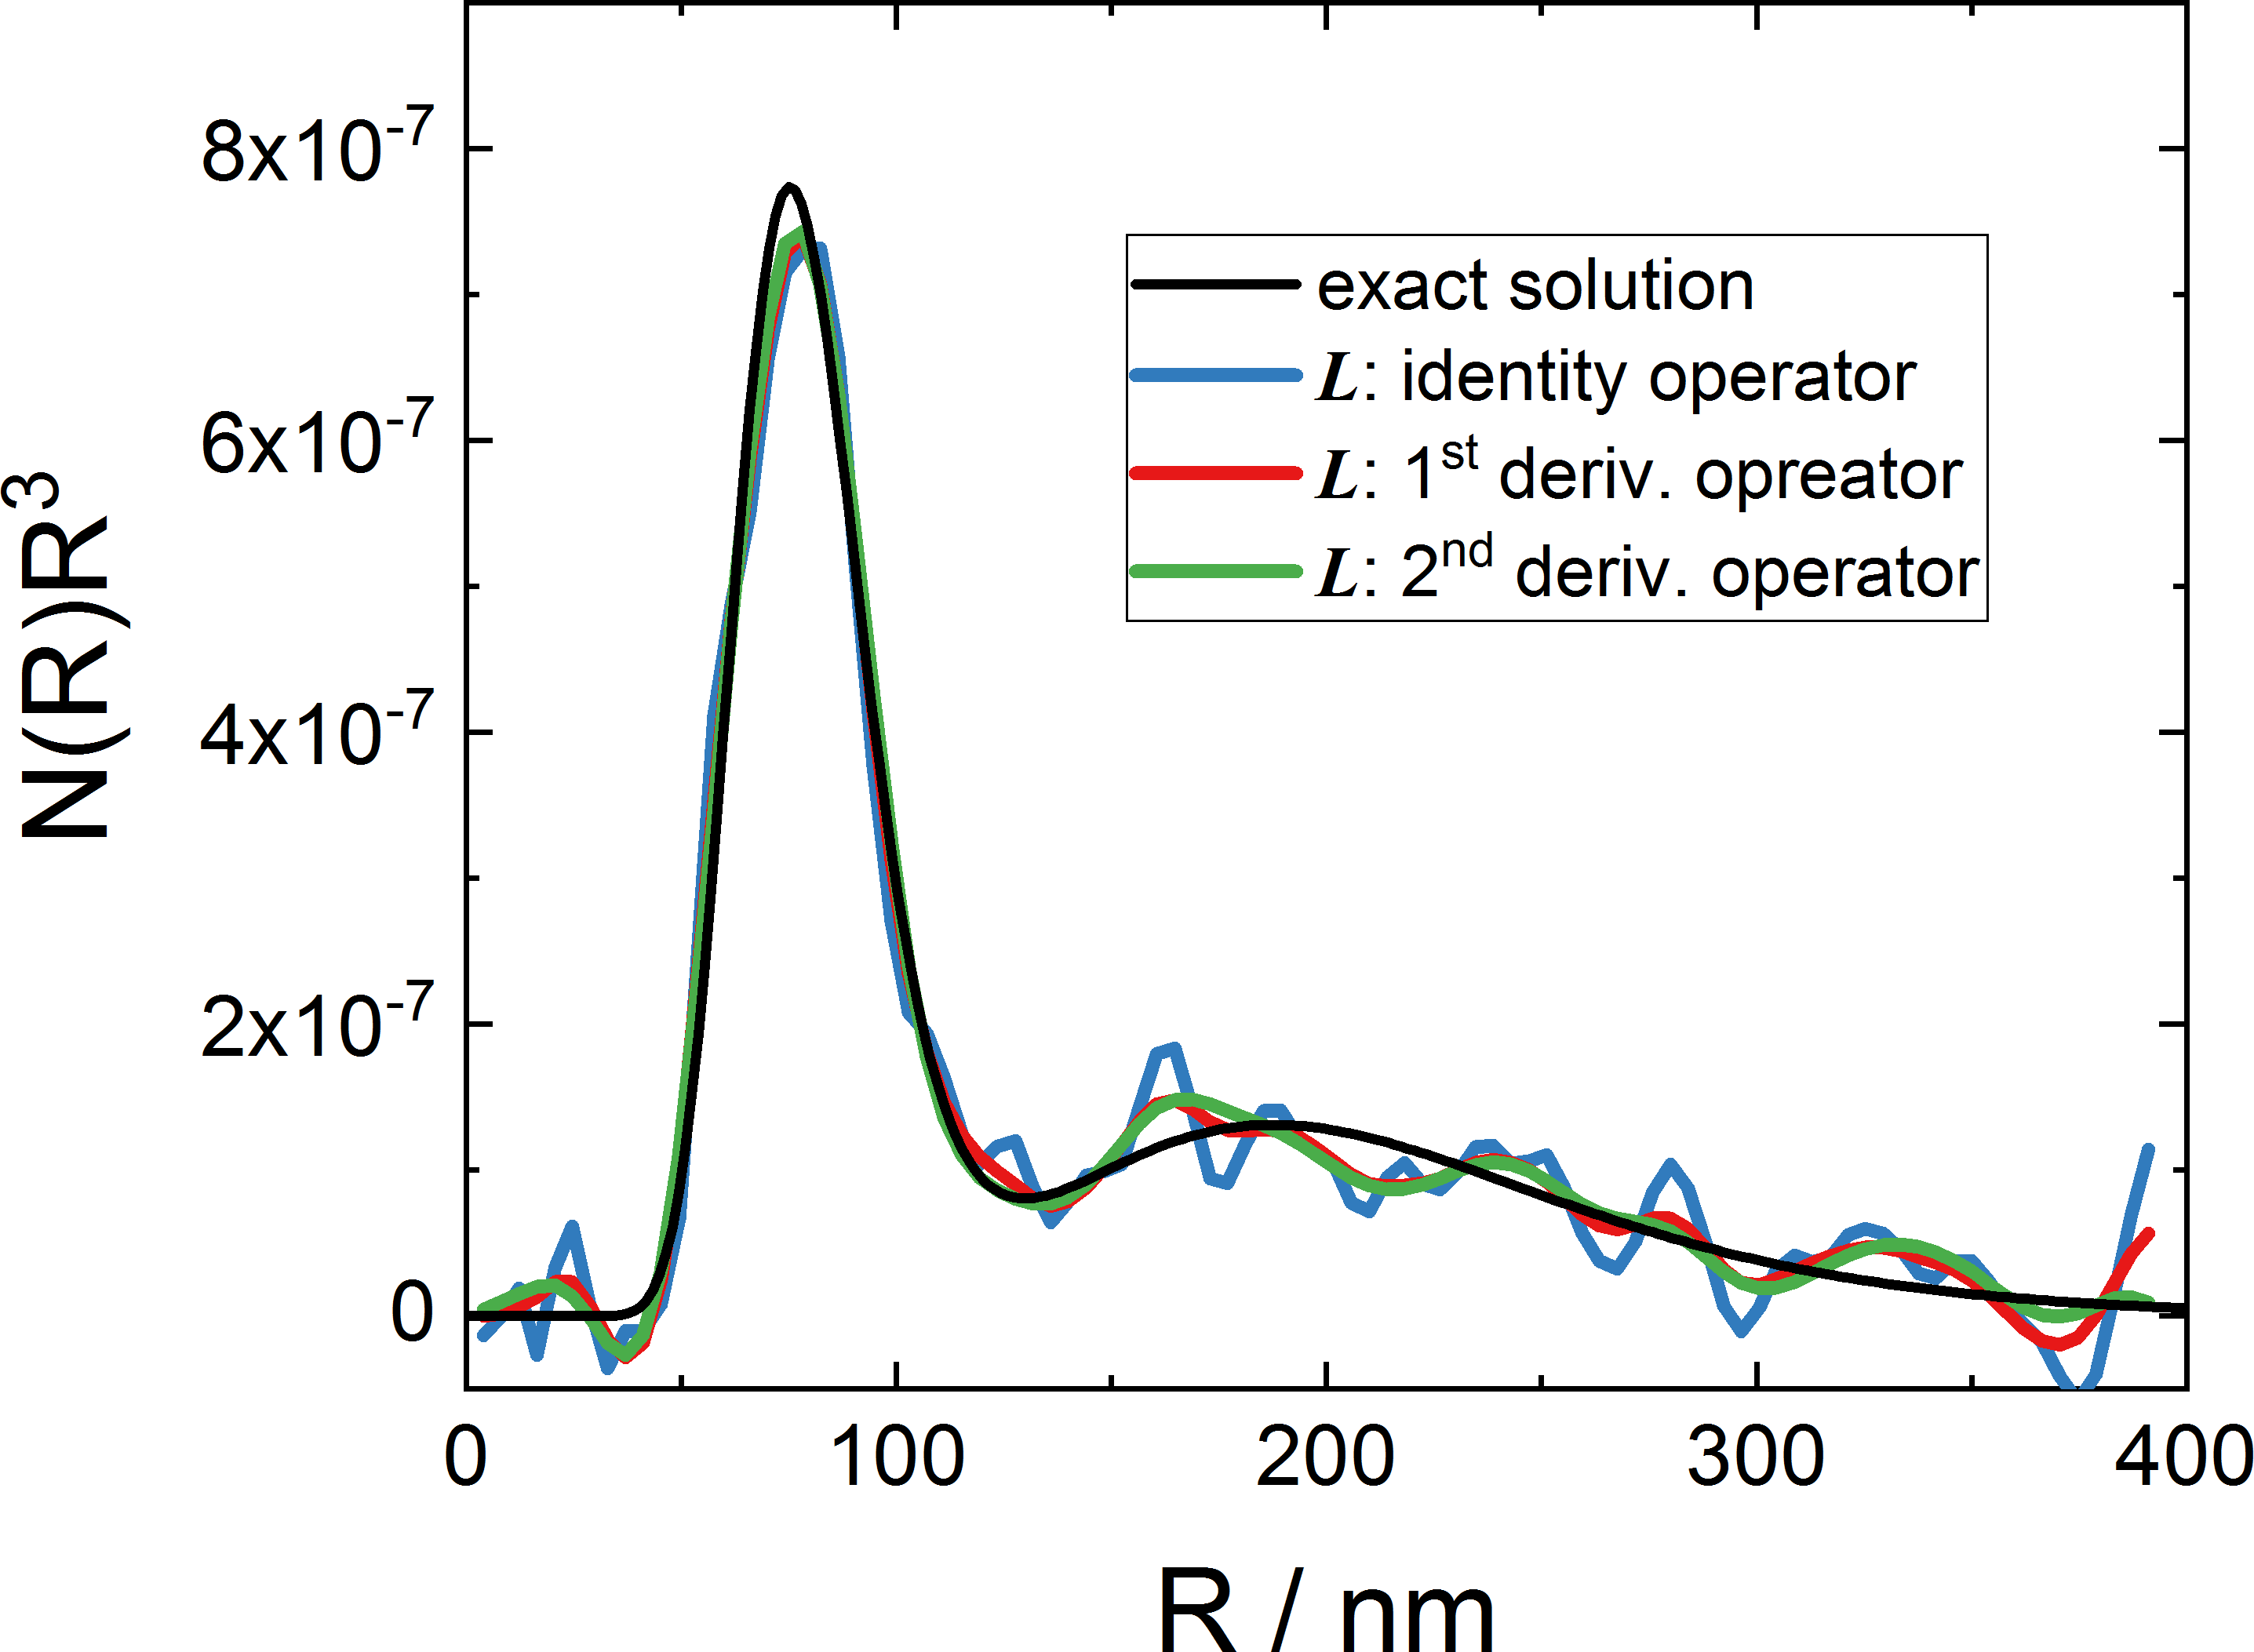
\includegraphics[width=0.45\textwidth]{../images/form_factor/EM/LLS_NRR3_GCVminimum.png}
\caption{The optimum Lagrange parameters $\lambda$ have been obtained by minimizing the ``Generalized Cross Validation'' function.\label{fig:EMGCVminimum}}
\end{figure}


\section{Non-negative linear least square regularization (NNLLS)}\label{sec:NNLLS}
The non-negative linear least square solver used here is taken from \cite{Lawson1995a} and are also available at netlib under
\url{http://www.netlib.org/lawson-hanson/} as Fortran source code which has been translated to C by \hyperref[https://www.netlib.org/f2c/]{f2c}. \SASfit is using this routine to solves the same ill-posed problems including a regularization term as in eq.\ \ref{eq:LLSreg} of section \ref{sec:LLS} just with an additional constrain of non-negativity.


\clearpage
\section{Maximum entropy method (MEM)}
entropy $S$:
\begin{align}
S&= \sum_{j=0}^{N-1} -x_j\ln\left(x_j/m_j\right) +x_j-m_j
\end{align}
with $\mathbf{m}$ being the prior estimate of $\mathbf{x}$.




\subsection{Jacobian and Hessian of mean square of the weighted deviations $\chi_r^2$}

Jacobian of $\chi_r^2$
\begin{align}
  \nabla \chi^2 &= 2\hat{\mathbf{A}}^T\hat{\mathbf{w}}^T\hat{\mathbf{w}}\hat{\mathbf{A}}\mathbf{x}-2\hat{\mathbf{A}}^T\hat{\mathbf{w}}^T\hat{\mathbf{w}}\mathbf{b}
\end{align}
Hessian of $\chi^2$
\begin{align}
  \nabla^2 \chi^2 &= 2\hat{\mathbf{A}}^T\hat{\mathbf{w}}^T\hat{\mathbf{w}}\hat{\mathbf{A}}
\end{align}
Jacobian of entropy $S$:
\begin{align}
  \nabla  S &= \begin{pmatrix}
    -\ln \left(\frac{x_0}{m_0}\right) \\
   \vdots \\
    -\ln \left(\frac{x_{N-1}}{m_{N-1}}\right)
  \end{pmatrix}
\end{align}
Hessian of entropy $S$:
\begin{align}
  \nabla^2  S &=
  \begin{pmatrix}
    -\frac{1}{x_0} & 0 & \dots & 0 \\
    0 & -\frac{1}{x_1} & \dots & 0 \\
    \vdots & \vdots & \ddots & \vdots \\
    0 & 0 & \dots & -\frac{1}{x_{N-1}}
  \end{pmatrix}
\end{align}


\section{Chahine inversion scheme}
Obtaining particle size distributions from forward scattered light using the Chahine inversion scheme has been introduced by \cite{Santer1983} and later on applied to SANS by \cite{Sen2014}.

\section{Inverse Rayleigh transform} 